\documentclass[utf8]{article}
\usepackage{amsmath,amssymb}
\usepackage{graphicx}
\usepackage{fullpage}
\usepackage{setspace}
\usepackage{verbatim}

\usepackage{algorithm}
\usepackage{algorithm}
\usepackage{algorithmicx}
\usepackage{algpseudocode}
\usepackage{amsmath}
\usepackage[top=2cm, bottom=2cm, left=2cm, right=2cm]{geometry}

\onehalfspacing

\usepackage{listings}
\usepackage{xcolor}
\definecolor{mGreen}{rgb}{0,0.6,0}
\definecolor{mGray}{rgb}{0.5,0.5,0.5}
\definecolor{mPurple}{rgb}{0.58,0,0.82}
\definecolor{backgroundColour}{rgb}{0.95,0.95,0.92}

\lstdefinestyle{CStyle}{
	backgroundcolor=\color{backgroundColour},   
	commentstyle=\color{mGreen},
	keywordstyle=\color{magenta},
	numberstyle=\tiny\color{mGray},
	stringstyle=\color{mPurple},
	basicstyle=\footnotesize,
	breakatwhitespace=false,         
	breaklines=true,                 
	captionpos=b,                    
	keepspaces=true,                 
	numbers=left,                    
	numbersep=5pt,                  
	showspaces=false,                
	showstringspaces=false,
	showtabs=false,                  
	tabsize=2,
	language=C
}

\title{\bf\huge Ray Tracing Renderer}
\author{Mei Yixuan}
\date{\today}

\begin{document}
\maketitle

\section{Introduction}
This document describes the design of a simple ray tracing renderer, along with some sample scenes rendered using it. I finished it as course project for Advanced Computer Graphics, given by Prof. Shimming Hu in Tsinghua University.

Complete code for this renderer can be found in https://github.com/AntonyMei/RayTracingRender, along with all external libraries and resources. This code is designed for this course project only and implies no warranty, use at your own risk. All code follow Apache License 2.0, except those external libraries and resources.

\section{Results}
This section shows some of the demo scenes rendered using this renderer. All scenes are rendered under 3840 * 2160 (or 3840 * 3840 if aspect ratio is 1) with more than 1000 samples per pixel and tracing depth 50.

\subsection{Hollow Glass Ball}
\begin{figure}[H]
	\centering
	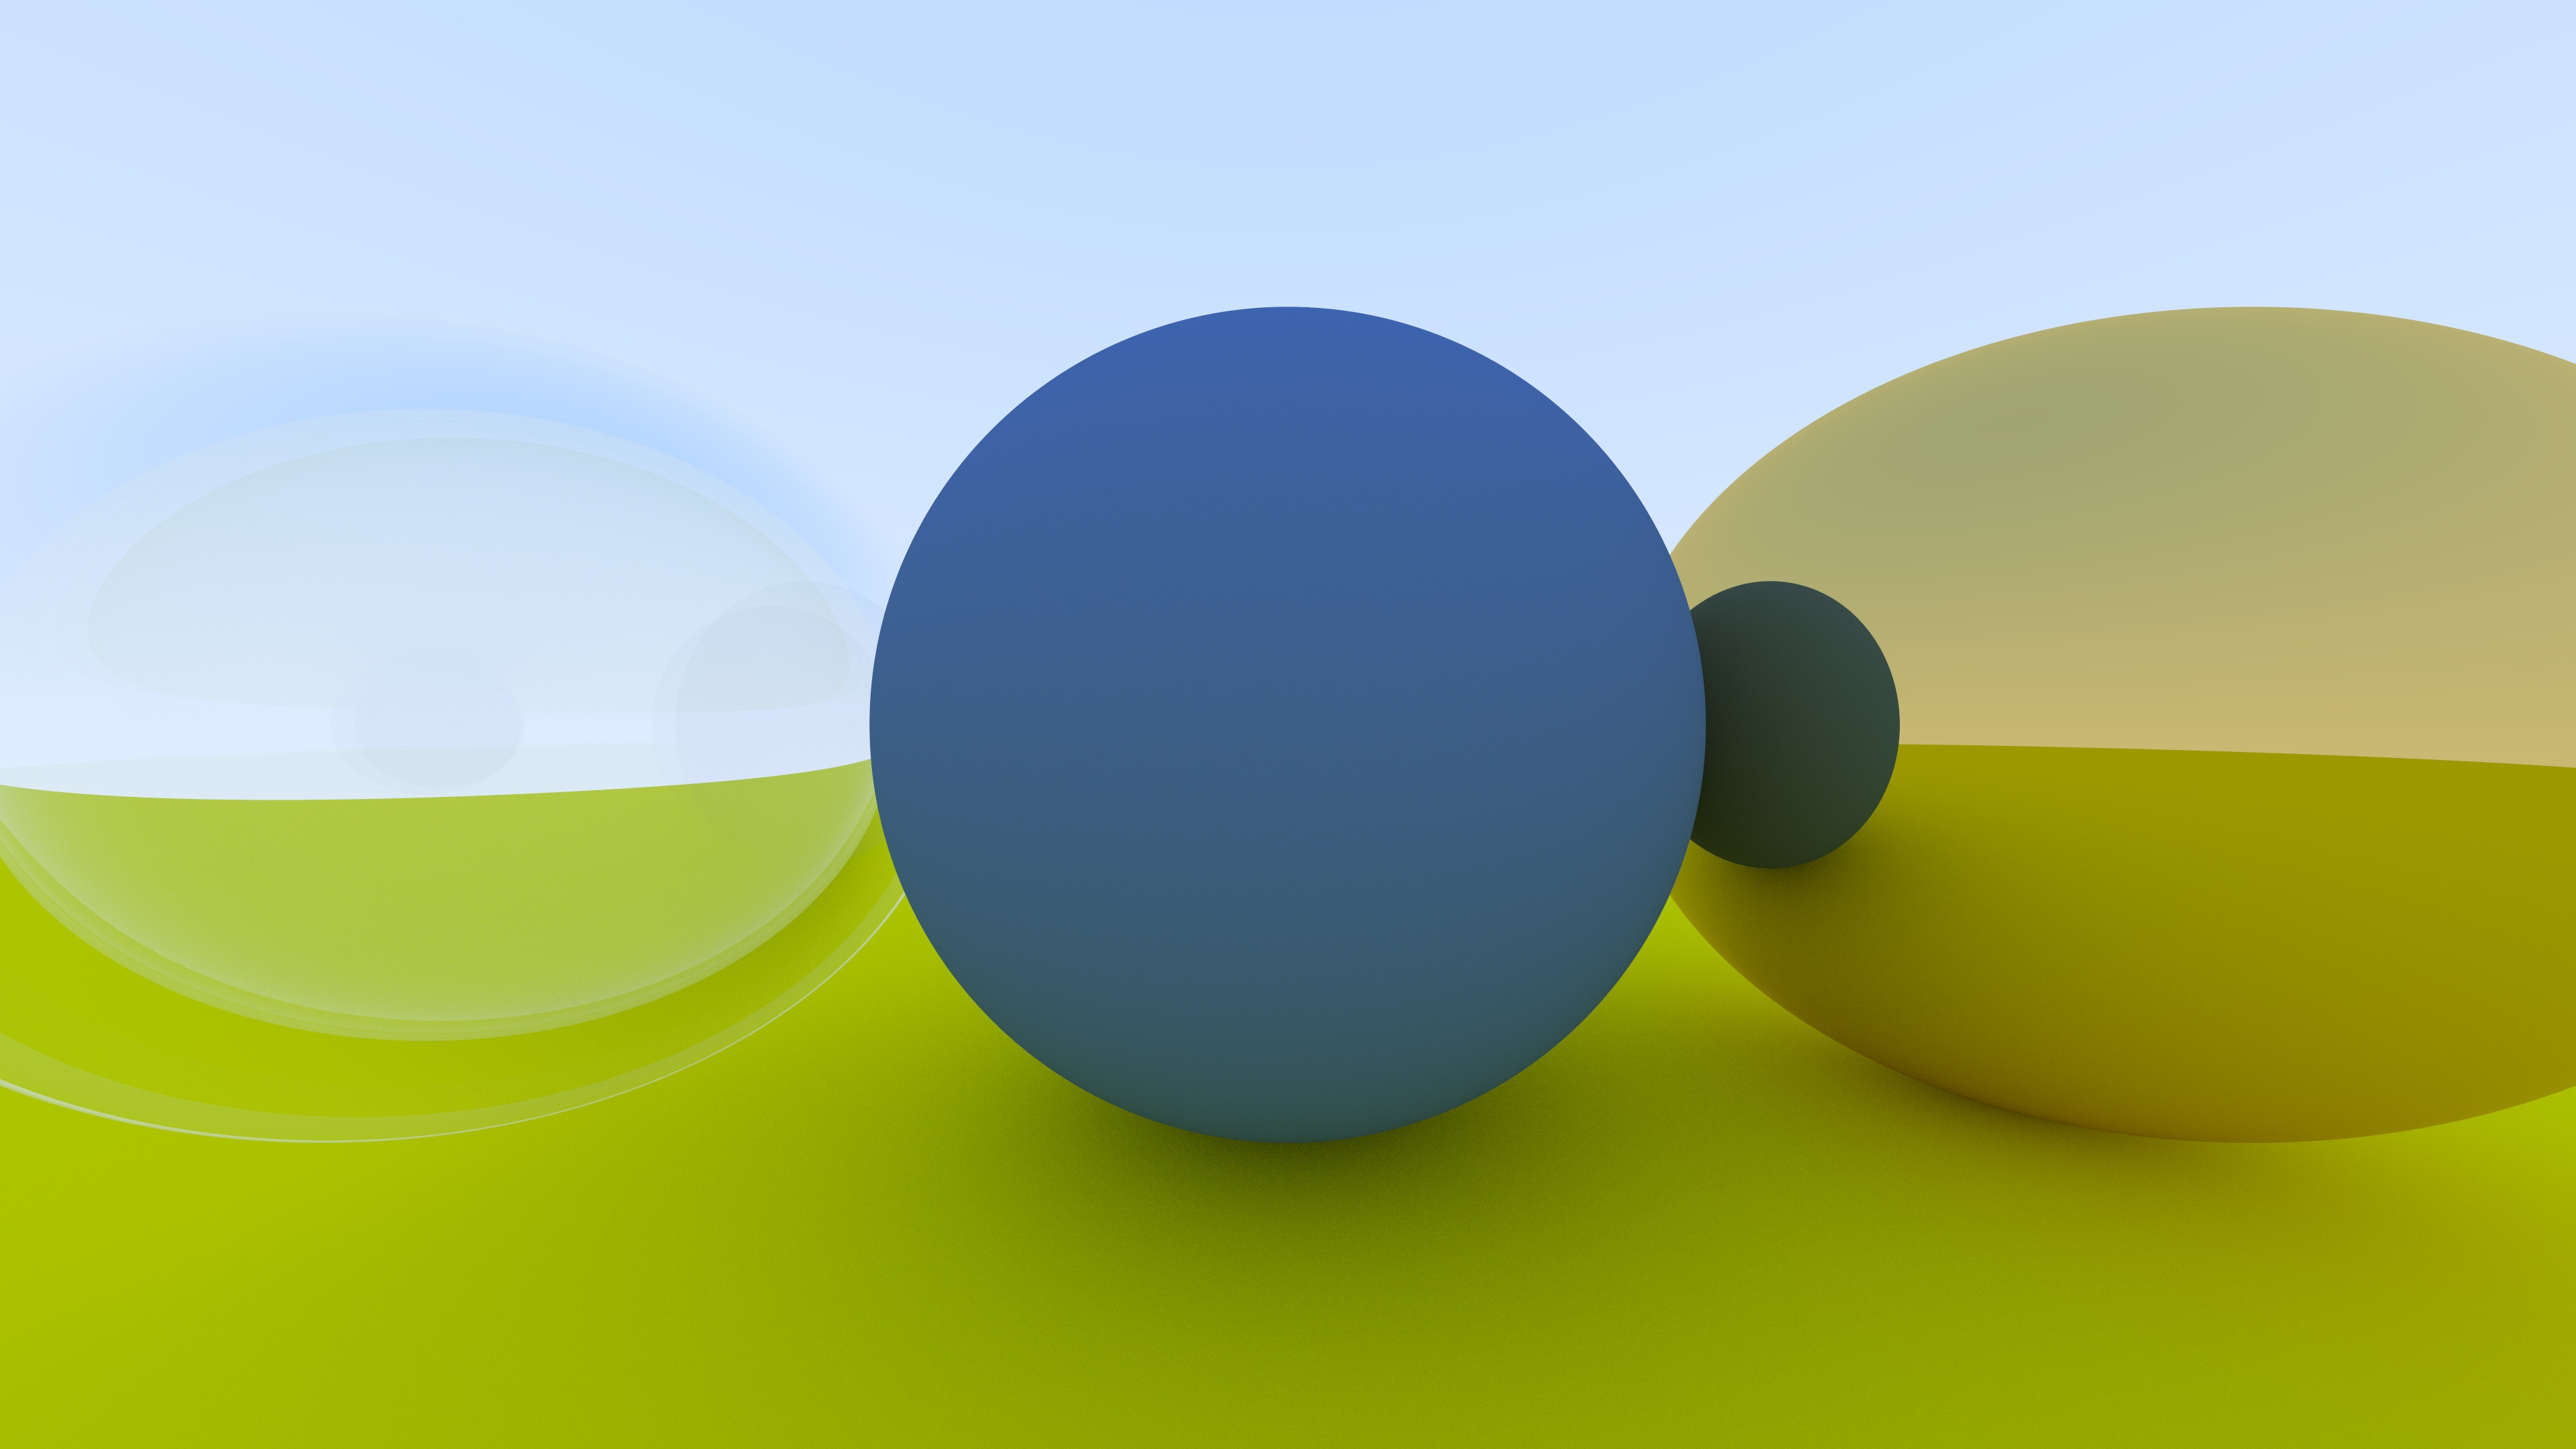
\includegraphics[width=0.7\linewidth]{../_results/hollow_glass_ball}
	\caption{Hollow Glass Ball}
	\label{fig:hollowglassball}
\end{figure}
This scene shows the usage of Lambertian (pure diffuse), Metallic (pure reflection) and Dielectric (refraction) material.

\subsection{Hollow Glass Ball Small FOV}
\begin{figure}[H]
	\centering
	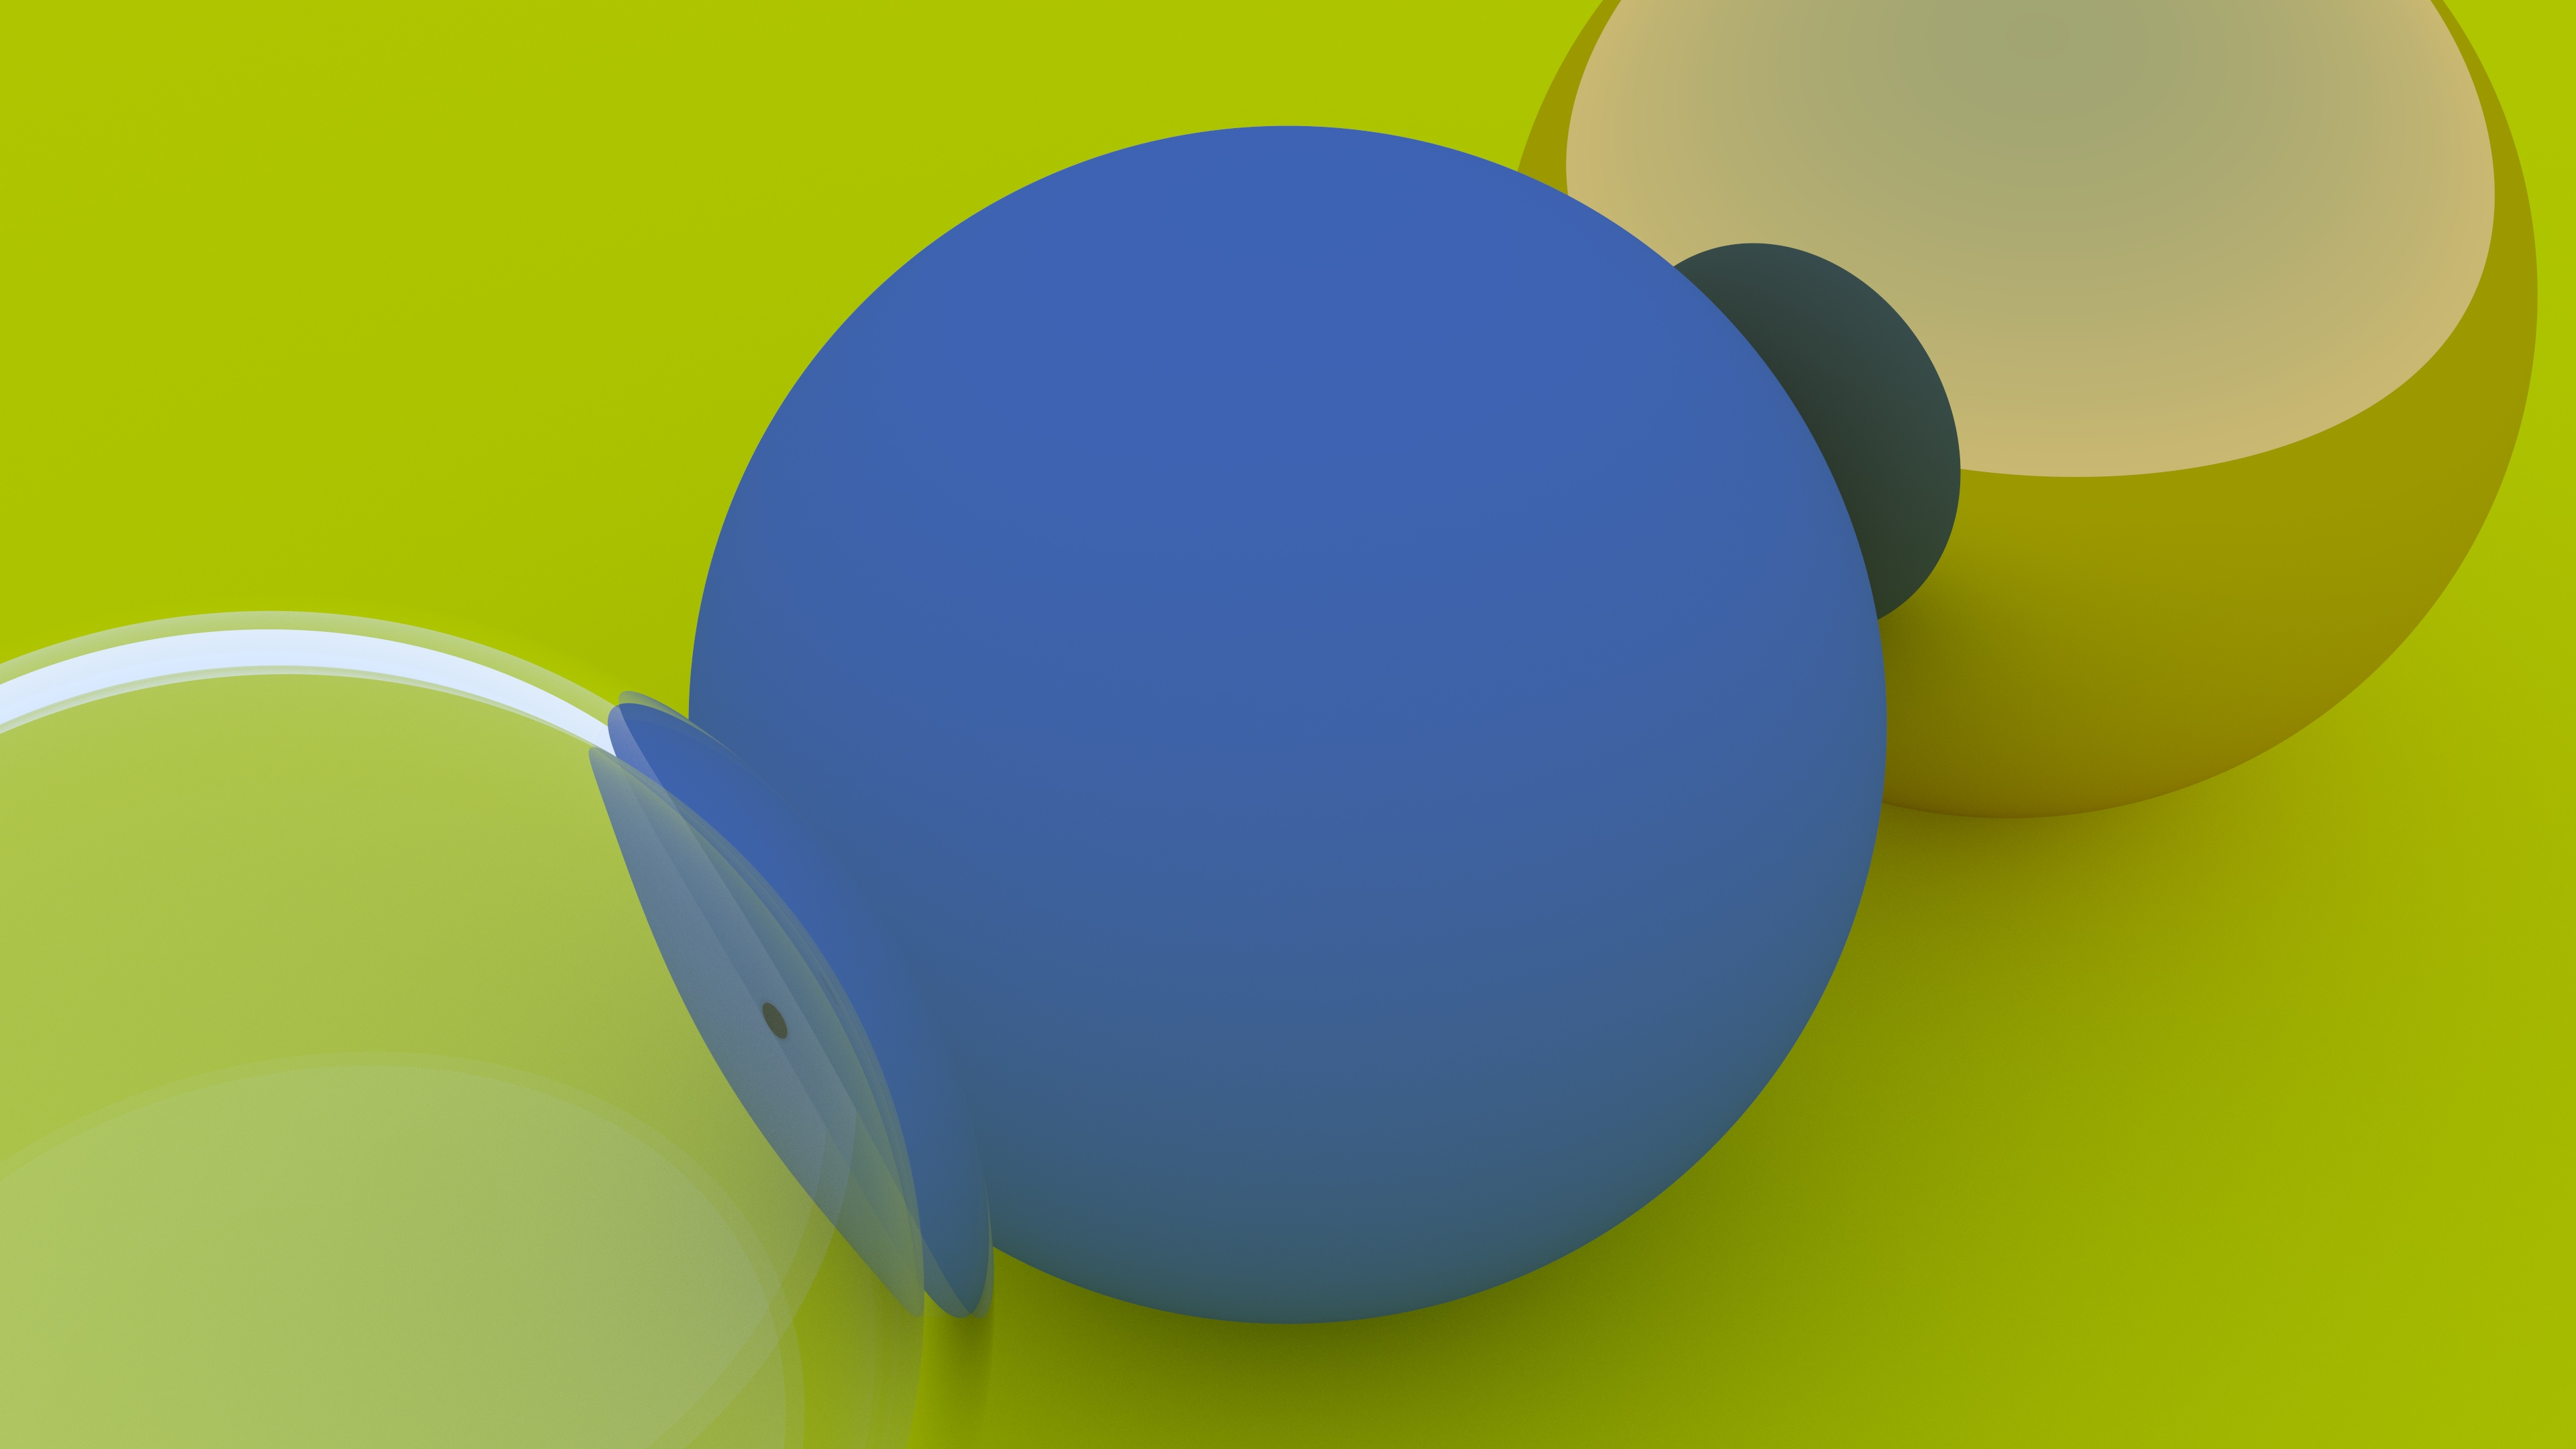
\includegraphics[width=0.7\linewidth]{../_results/hollow_glass_ball_small_fov}
	\caption{Hollow Glass Ball Small FOV}
	\label{fig:hollowglassballsmallfov}
\end{figure}
This scene is identical to the last one, but with smaller camera FOV. Note that edge of the dielectric ball has reflection rather than refraction, which is physically accurate.

\subsection{Hollow Glass Ball Off Focus}
\begin{figure}[H]
	\centering
	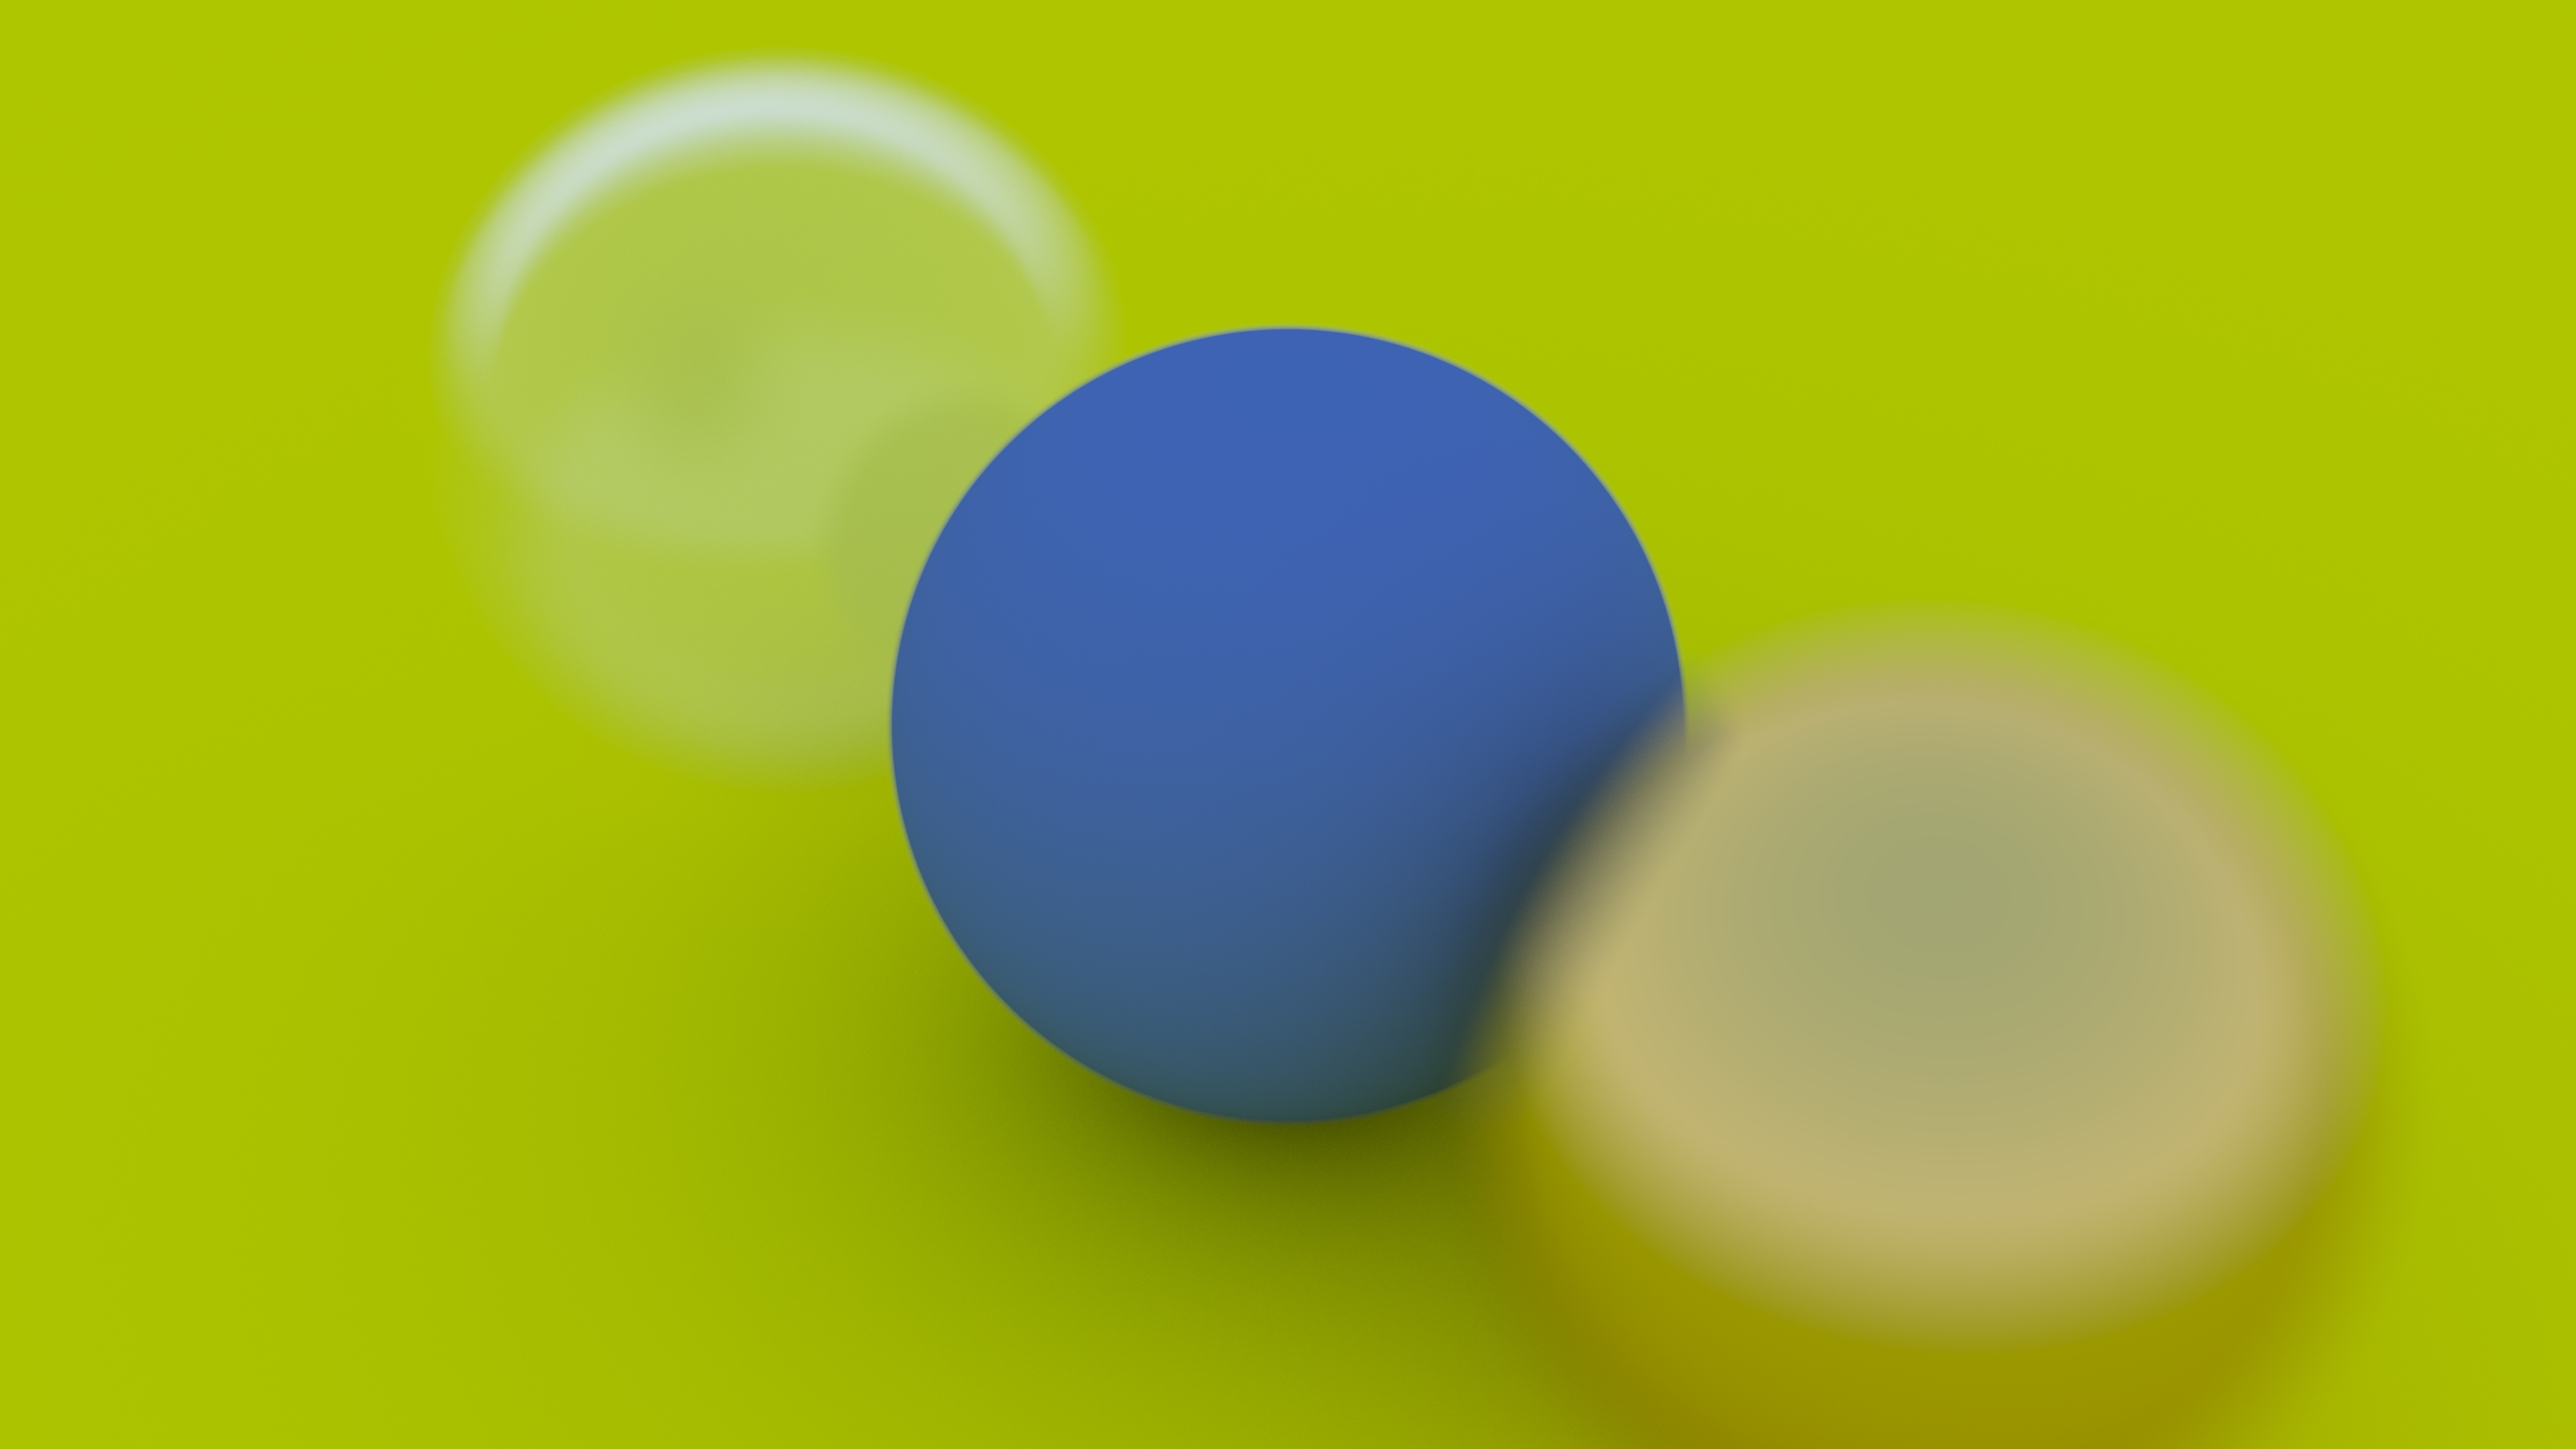
\includegraphics[width=0.7\linewidth]{../_results/hollow_glass_ball_off_focus}
	\caption{Hollow Glass Ball Off Focus}
	\label{fig:hollowglassballofffocus}
\end{figure}
This scene shows off-focus blur effect.

\subsection{Many Balls}
\begin{figure}[H]
	\centering
	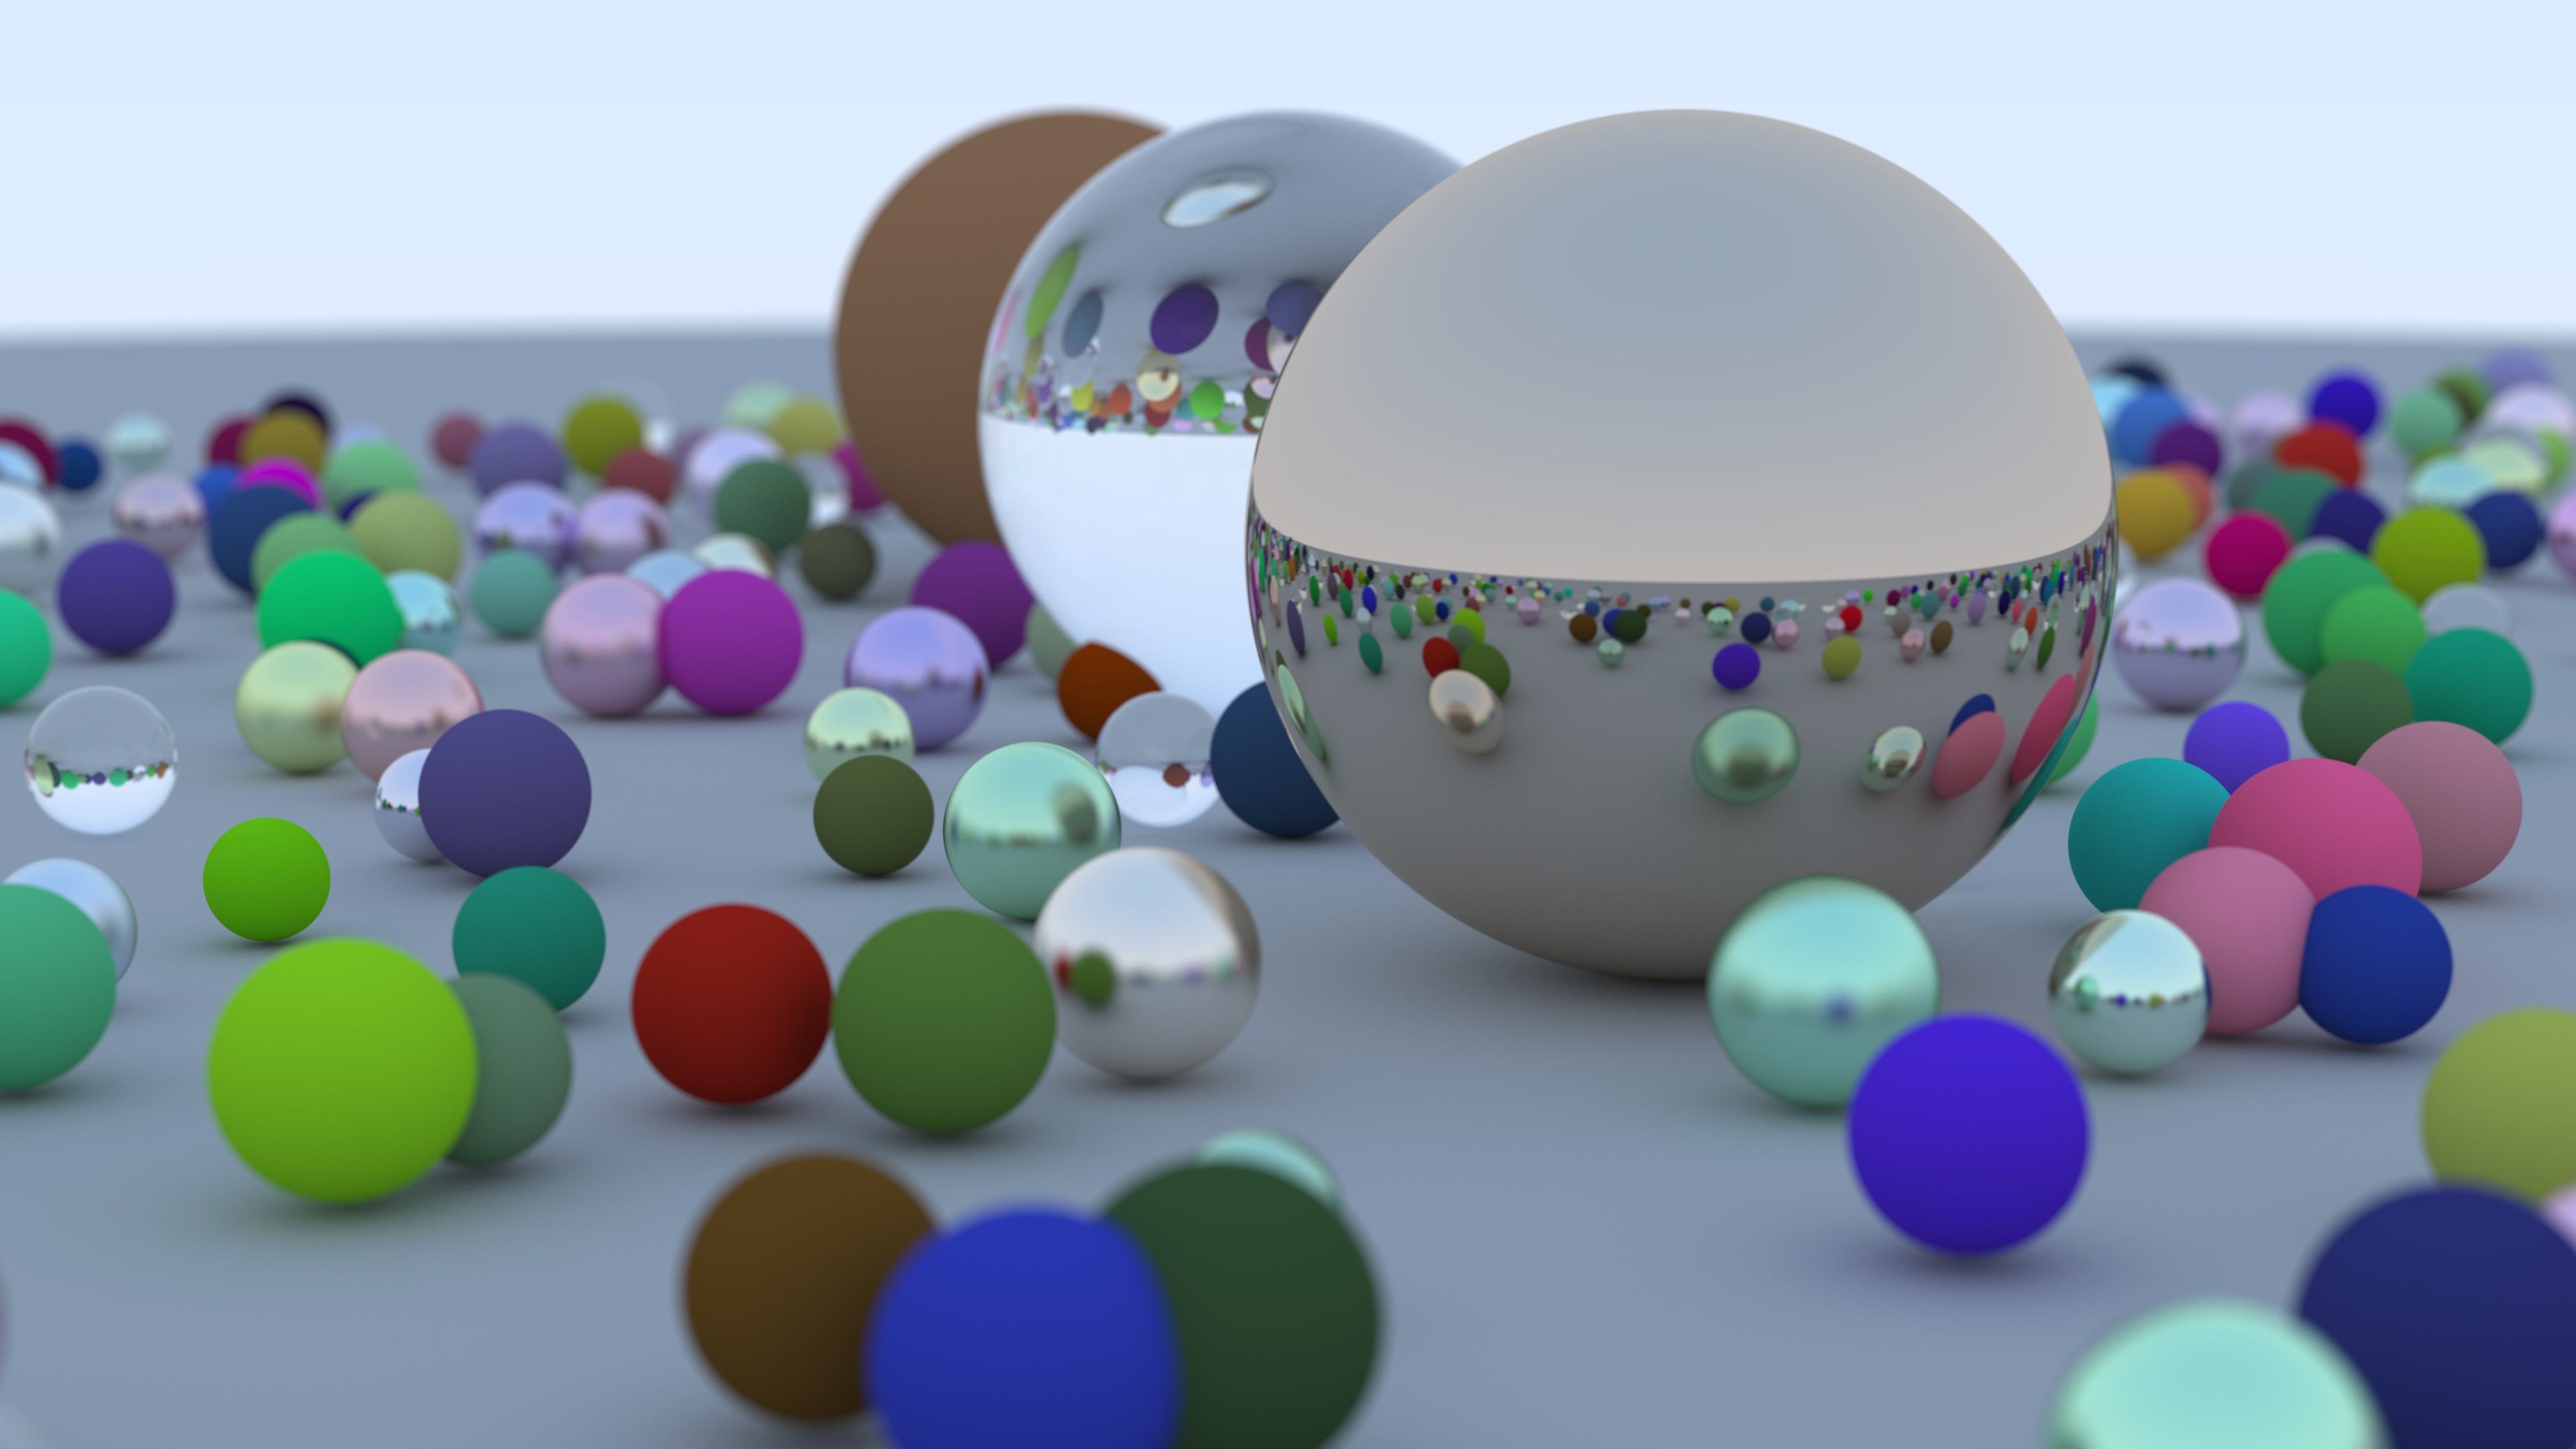
\includegraphics[width=0.7\linewidth]{../_results/many_balls}
	\caption{Many Balls}
	\label{fig:manyballs}
\end{figure}
This scene contain many balls. Note that metallic material can use fuzziness to simulate imperfect reflection.

\subsection{Motion Blur}
\begin{figure}[H]
	\centering
	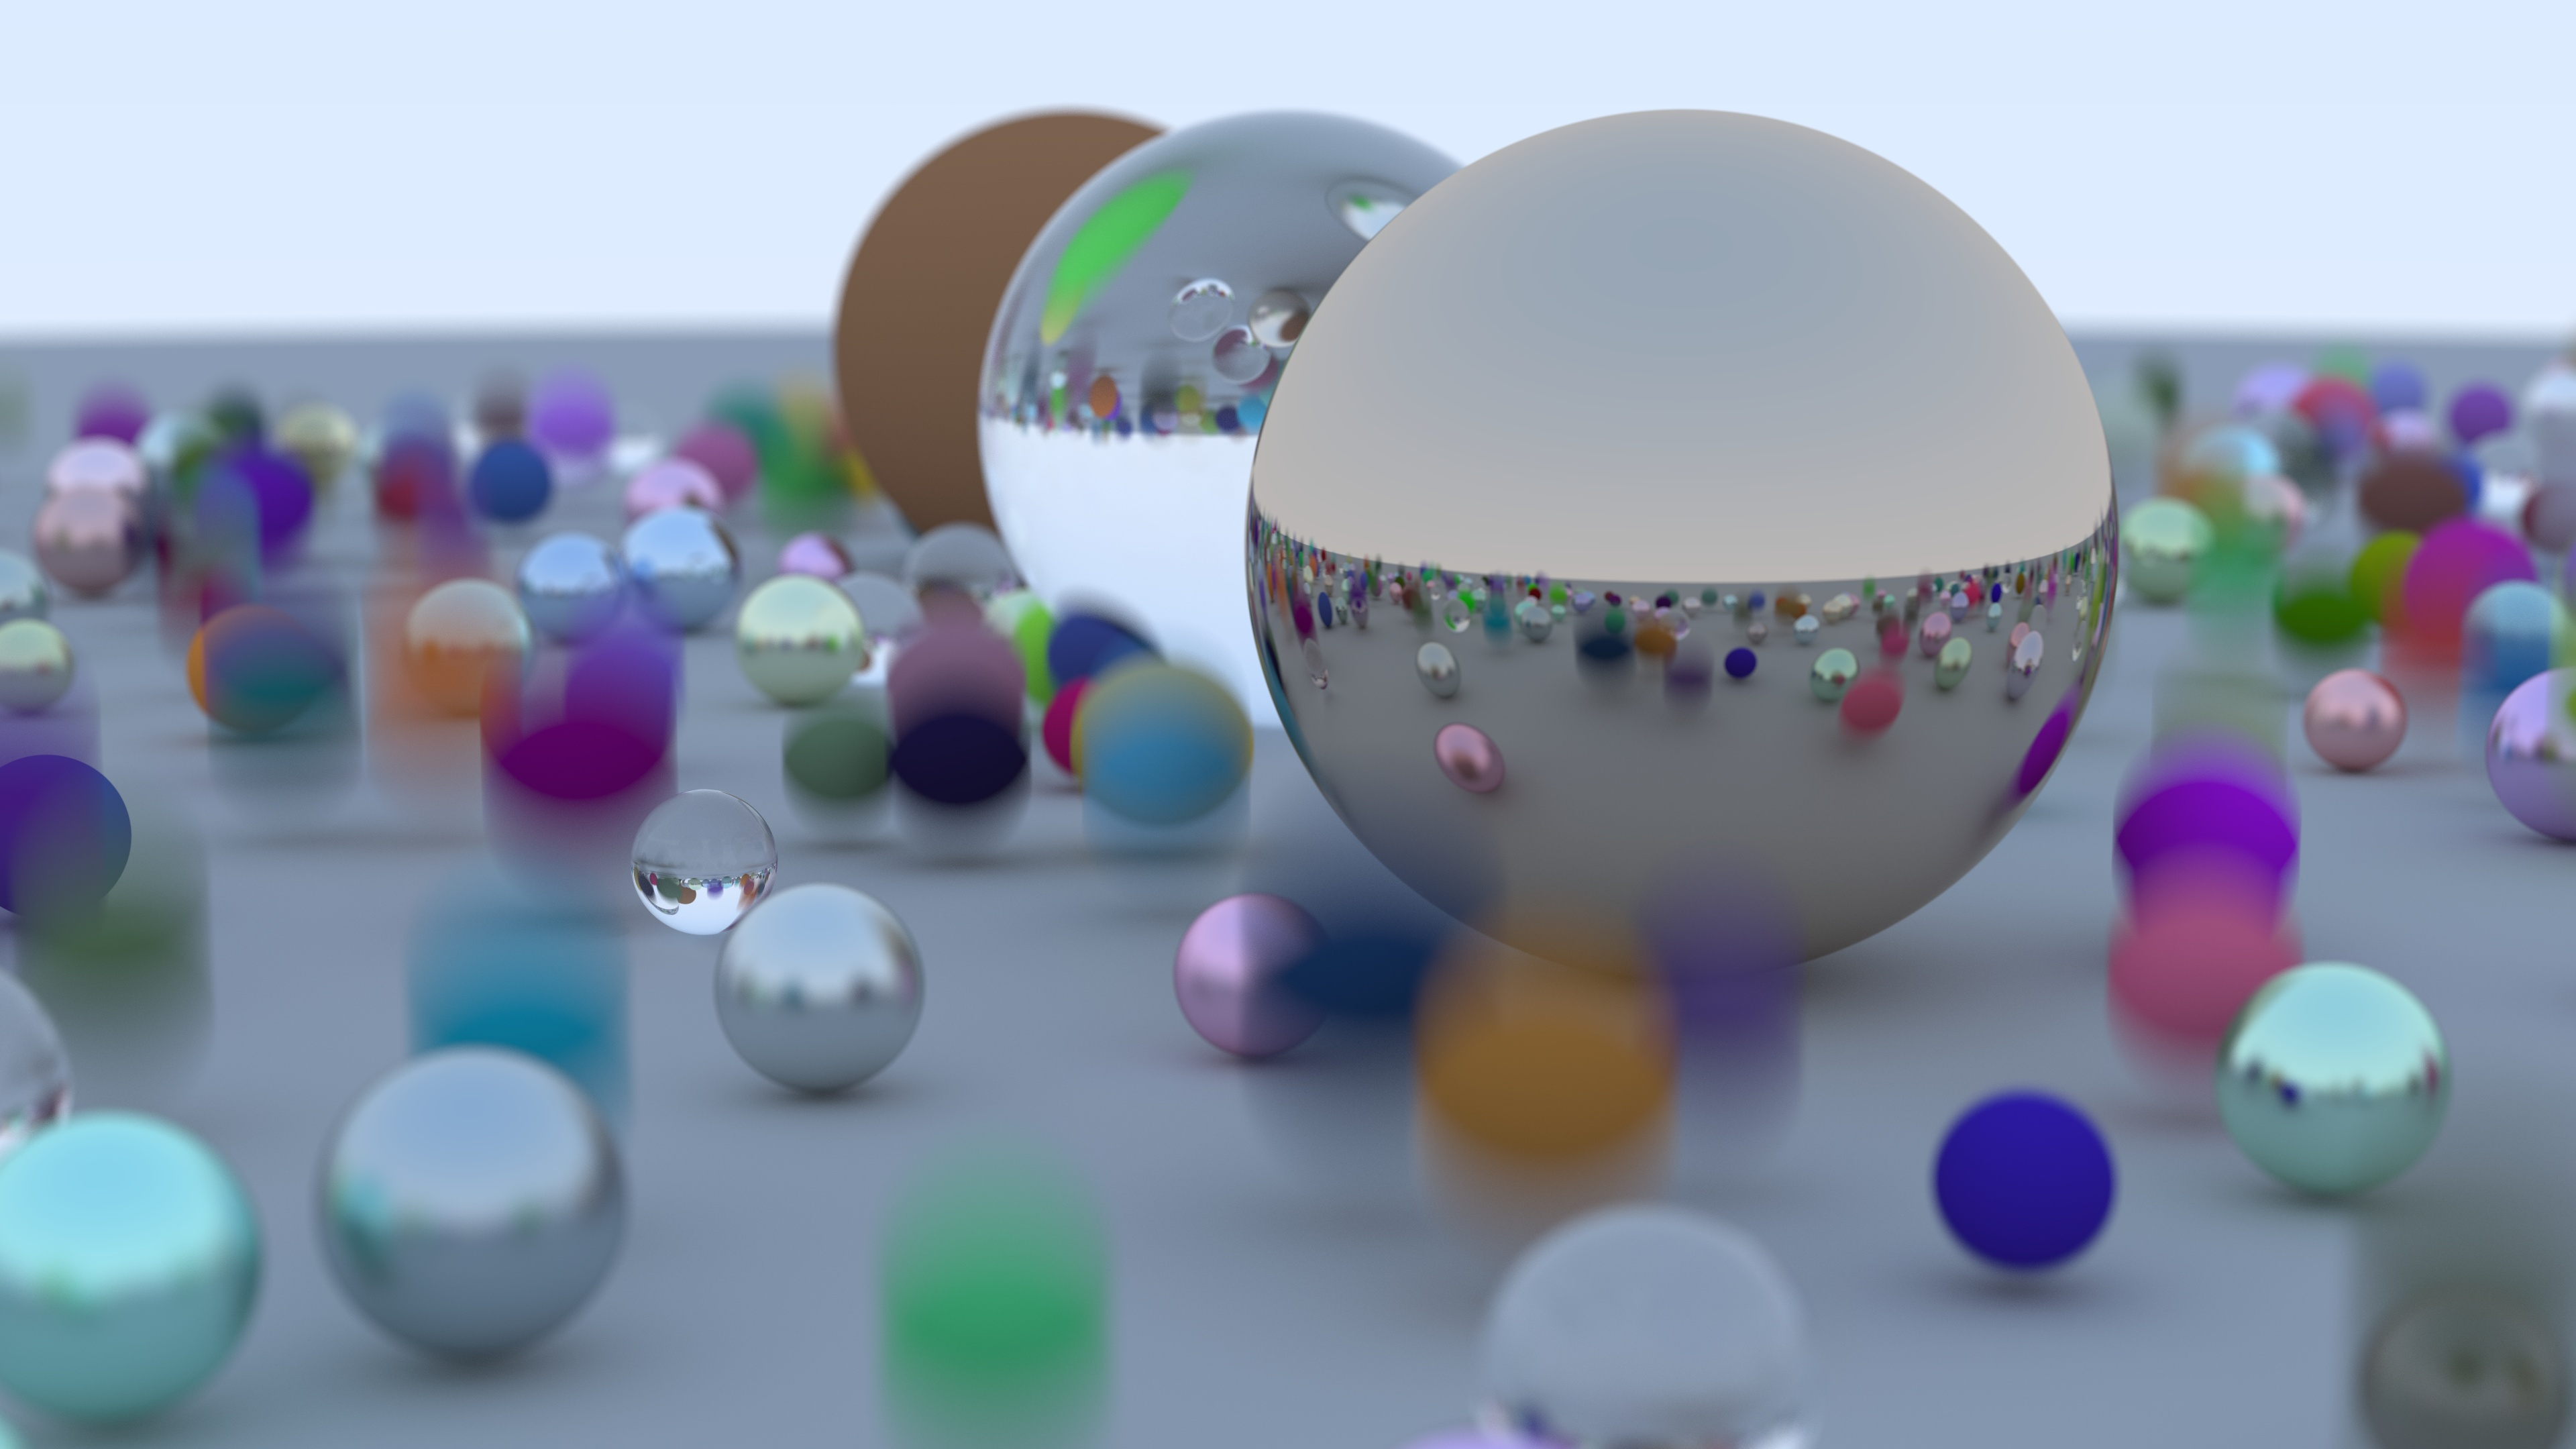
\includegraphics[width=0.7\linewidth]{../_results/motion_blur}
	\caption{Motion Blur}
	\label{fig:motionblur}
\end{figure}
This scene shows motion blur effect.

\subsection{Motion Blur Checker}
\begin{figure}[H]
	\centering
	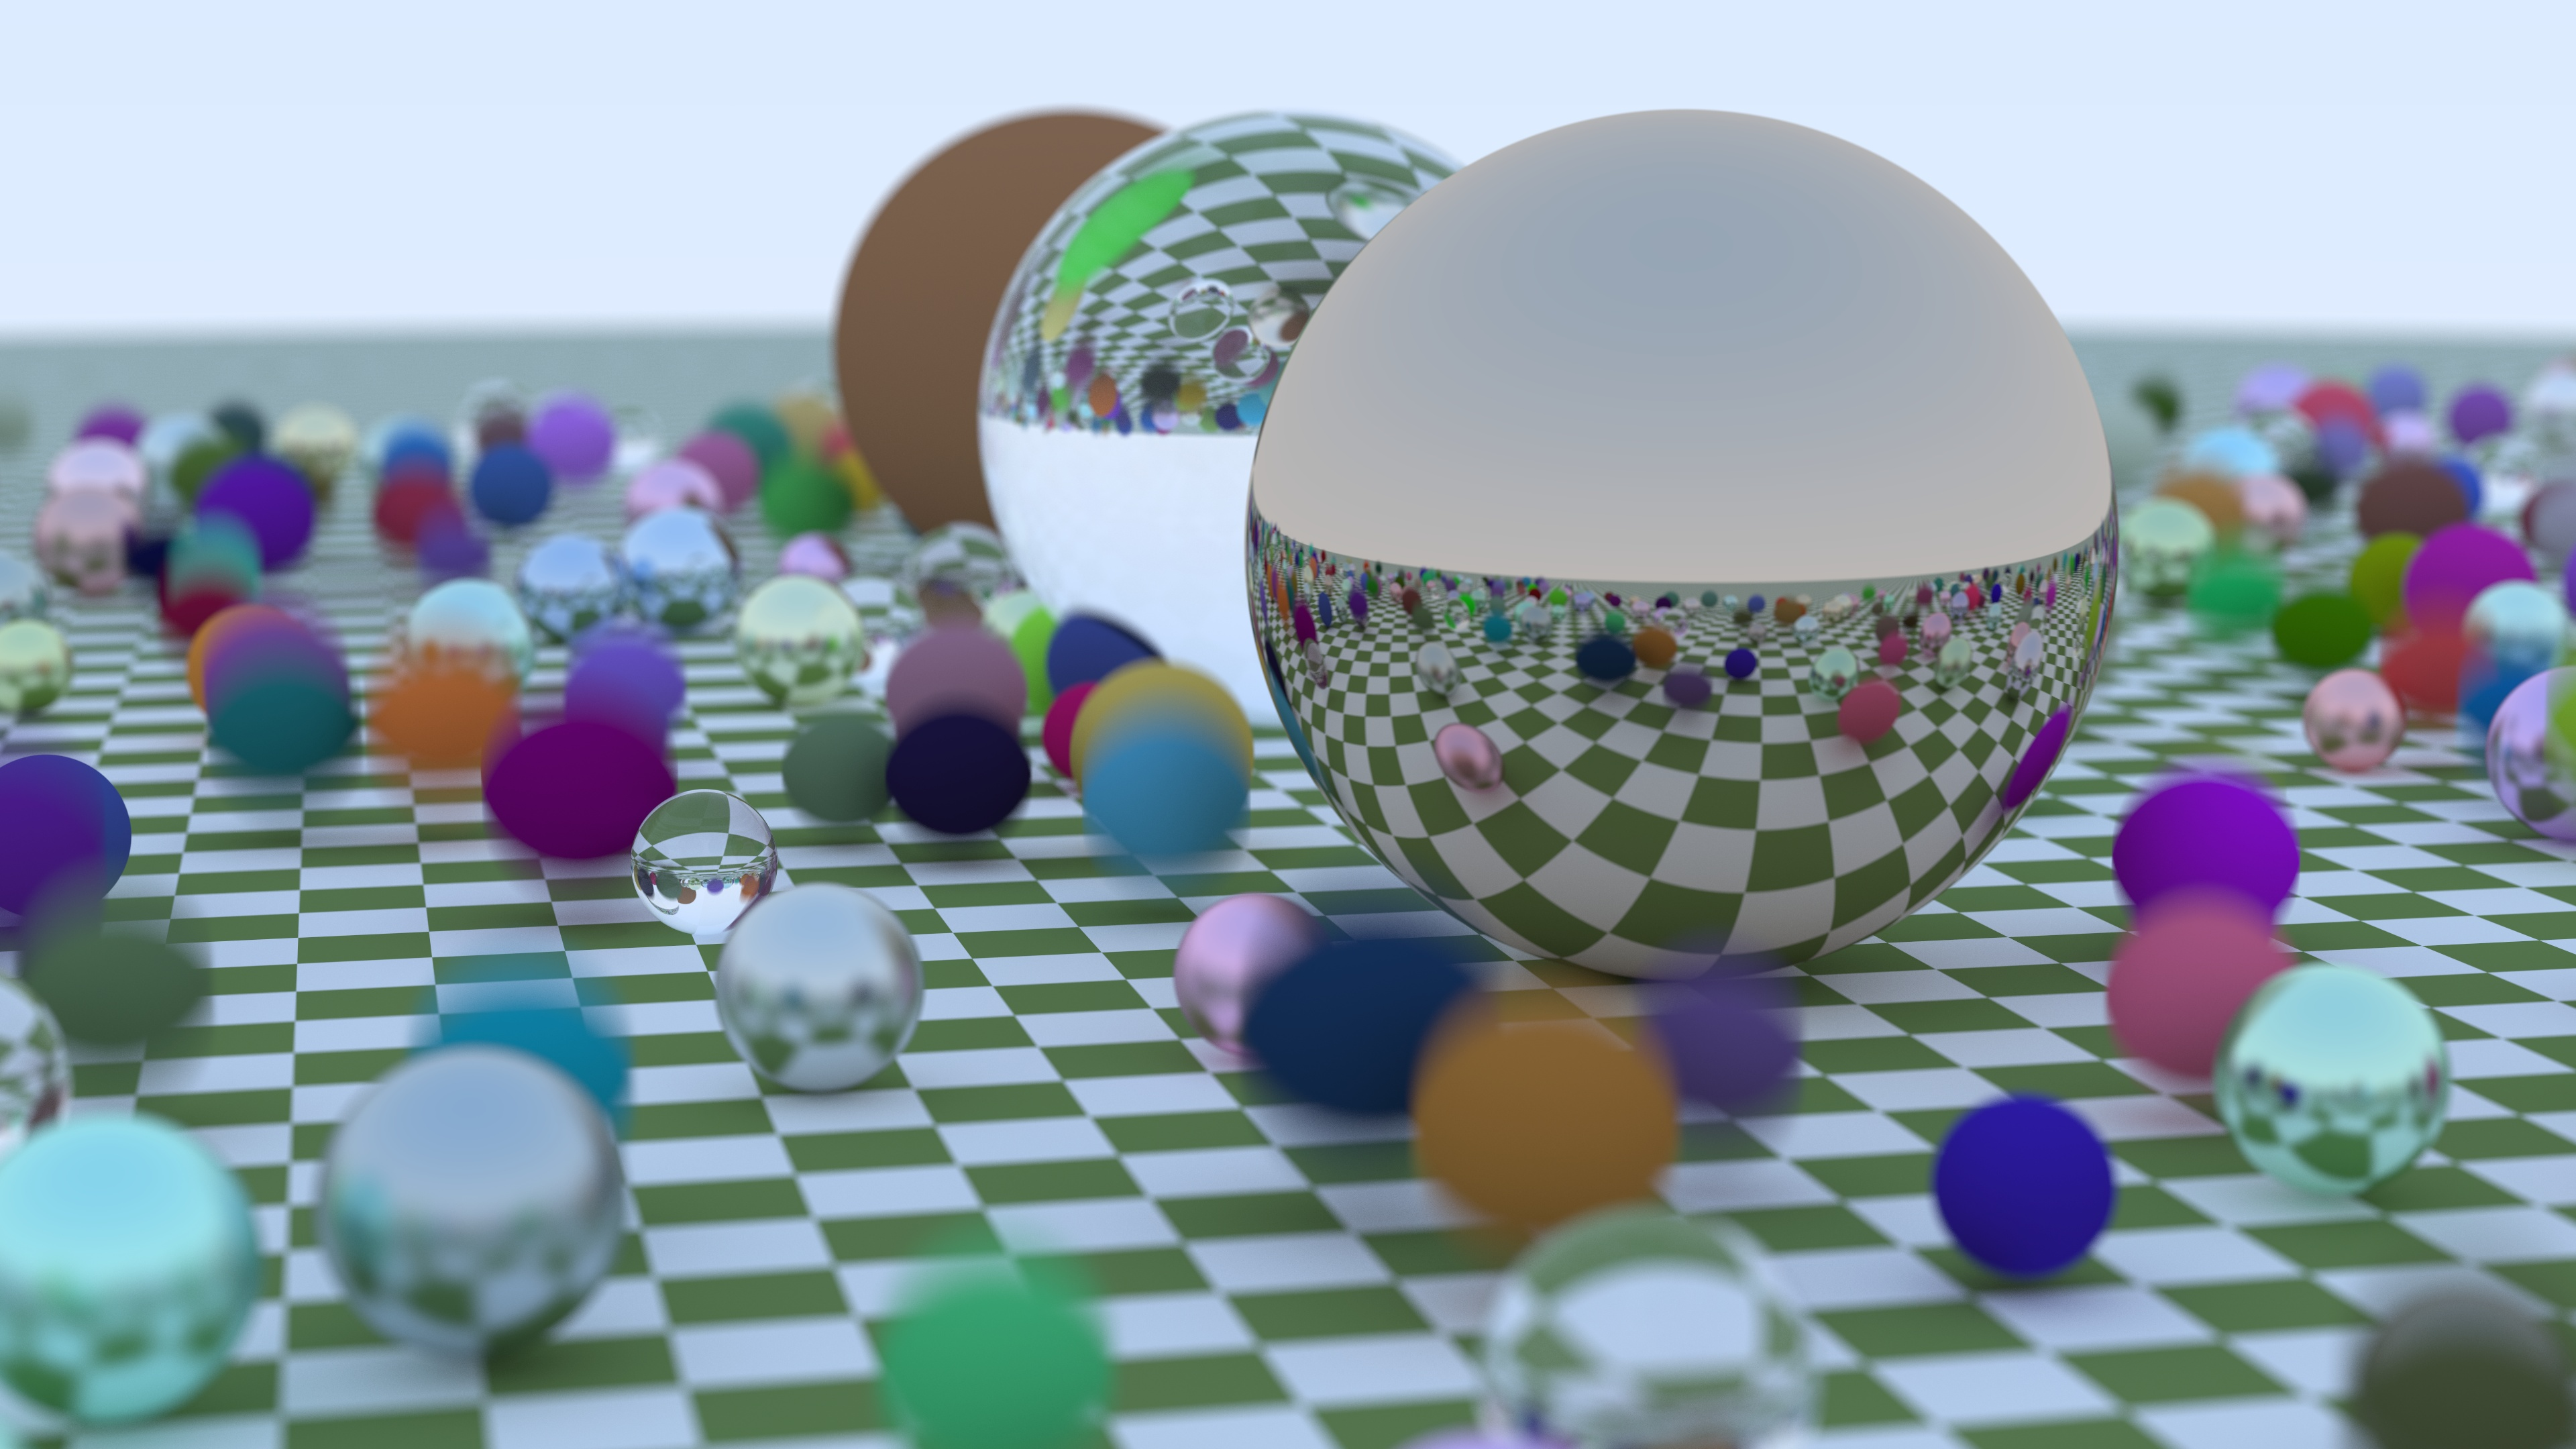
\includegraphics[width=0.7\linewidth]{../_results/motion_blur_checker}
	\caption{Motion Blur Checker}
	\label{fig:motionblurchecker}
\end{figure}
This scene adds a simple procedural texture (checker texture) to the last one.

\subsection{Earth}
\begin{figure}[H]
	\centering
	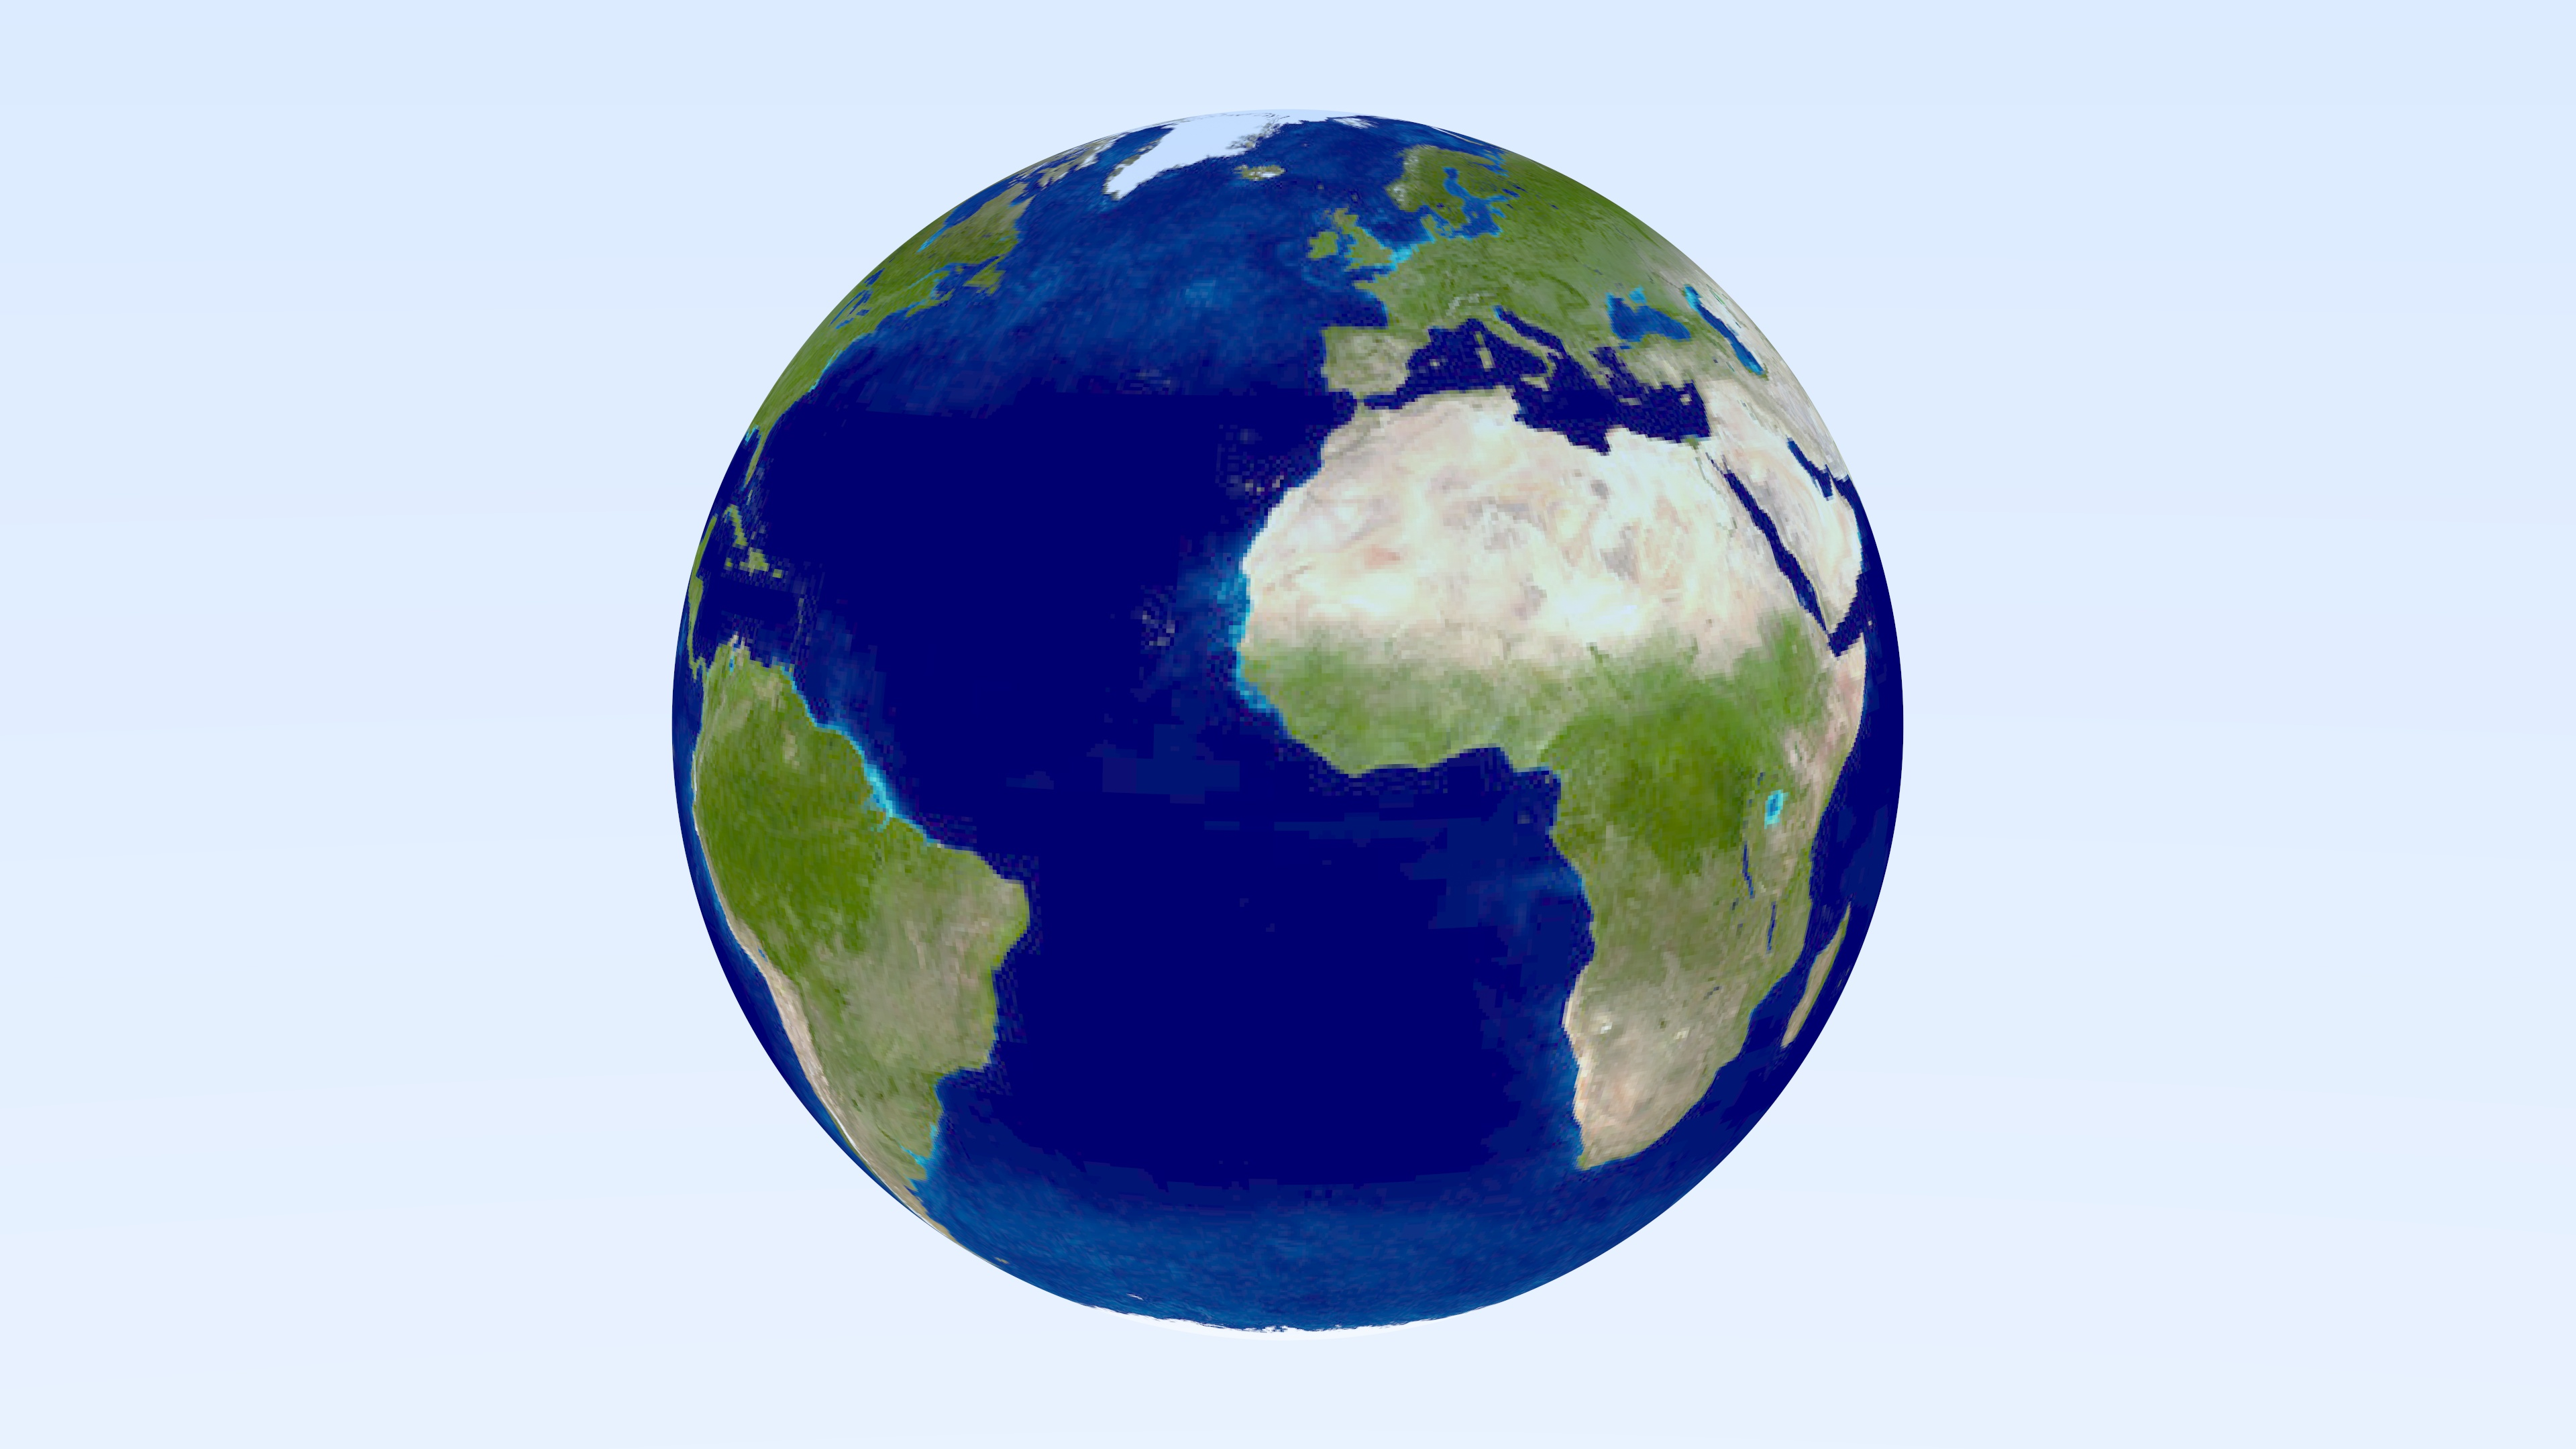
\includegraphics[width=0.7\linewidth]{../_results/earth}
	\caption{Earth}
	\label{fig:earth}
\end{figure}
This scene is a ball with image texture.

\subsection{Cornell Box Series}
\begin{figure}[H]
	\centering
	\includegraphics[width=0.5\linewidth]{../_results/cornell_box_empty}
	\caption{Cornell Box Empty}
	\label{fig:cornellboxempty}
\end{figure}
This is an empty Cornell Box constructed with axis-aligned rectangles.

\begin{figure}[H]
	\centering
	\includegraphics[width=0.5\linewidth]{../_results/cornell_box_two_blocks}
	\caption{Cornell Box Tow Blocks}
	\label{fig:cornellboxtwoblocks}
\end{figure}
\noindent
Added two boxes to the last scene.

\begin{figure}[H]
	\centering
	\includegraphics[width=0.5\linewidth]{../_results/cornell_box}
	\caption{Cornell Box}
	\label{fig:cornellbox}
\end{figure}
\noindent
Add rotation to the two boxes. Color bleeding is obvious on two surfaces facing walls.

\subsection{Cornell Box Participating Media}
\begin{figure}[H]
	\centering
	\includegraphics[width=0.5\linewidth]{../_results/cornell_box_participating_media}
	\caption{Cornell Box Participating Media}
	\label{fig:cornellboxparticipatingmedia}
\end{figure}
This scene replace the two original boxes with participating media boxes. These boxes are assigned with isotropic material to simulate the effect of smoke. This is a technique often used in volumetric rendering. 

\subsection{Book2 Final}
\begin{figure}[H]
	\centering
	\includegraphics[width=0.8\linewidth]{../_results/book_2_final}
	\caption{Book2 Final}
	\label{fig:book2final}
\end{figure}
This scene is a modified version of the one used by Peter Shirley in Ray Tracing Mini-Books 2. It combines may techniques. The whole scene is filled with thin smoke, rendered using participating media. The orange ball on the top left shows motion blur. The earth ball shows image textures. The marble ball in the middle is a complex example of procedural texture computed using Perlin noise. The box on the top right contains 10000 balls as components and use BVH to accelerate.

\subsection{Test Obj}
\begin{figure}[H]
	\centering
	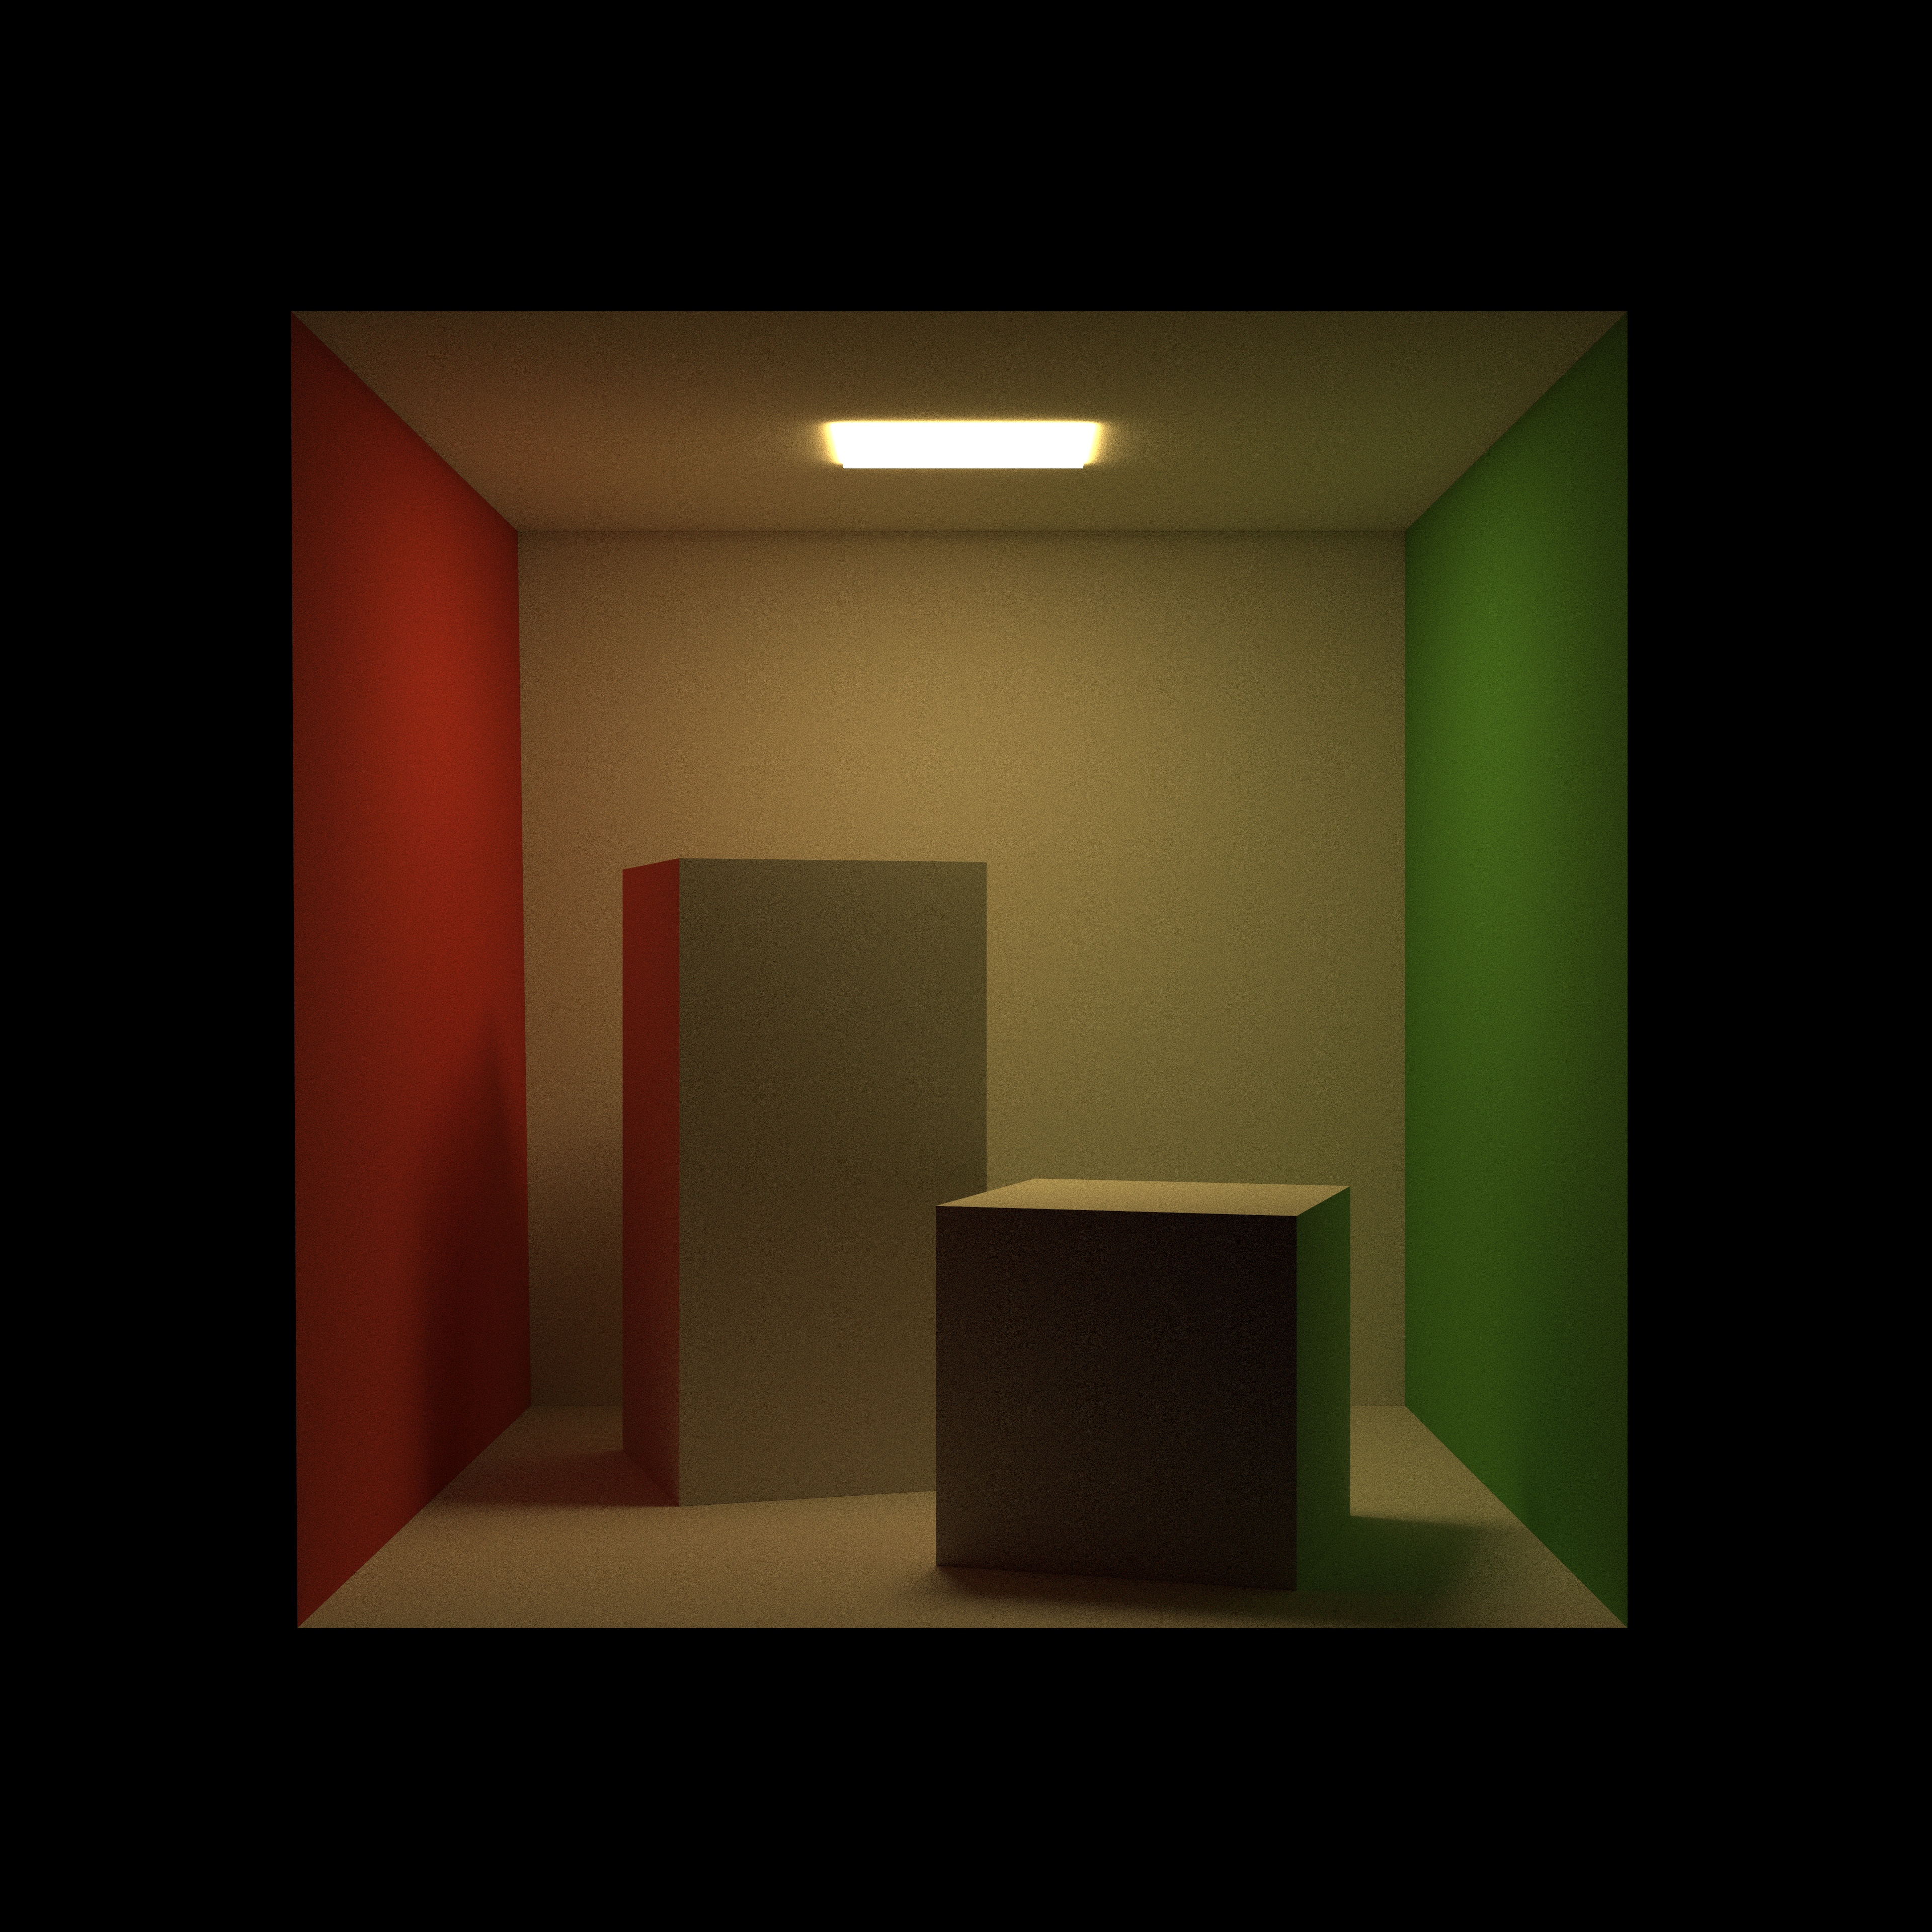
\includegraphics[width=0.45\linewidth]{../_results/test_obj}
	\caption{Test Obj}
	\label{fig:testobj}
\end{figure}
A simple scene used in obj test. This Cornell Box is made of triangles. It is stored in a .obj file (with material description in .mtl file) and imported using Tinyobjloader.

\subsection{Sponza Sun}
\begin{figure}[H]
	\centering
	\includegraphics[width=0.45\linewidth]{../_results/sponza_sun}
	\caption{Sponza Sun}
	\label{fig:sponzasun}
\end{figure}
This scene is a more complicated one with image textures. Note that in this scene, a biased sampling technique is used such that the sun gets more samples.

\subsection{Sponza Crytek Series}
\begin{figure}[H]
	\centering
	\includegraphics[width=0.8\linewidth]{../_results/sponza_crytek_cloudy}
	\caption{Sponza Crytek Cloudy}
	\label{fig:sponzacrytekcloudy}
\end{figure}
This scene is a remastered version of the last one from Crytek cooperation. It is rendered unbiasedly with Path Tracing. Note that bump map is enabled to add more details to the geometry (like the lion in the back). The following one is the same scene with a more complicated skybox. It can be used to simulate extremely sunny weather.

\begin{figure}[H]
	\centering
	\includegraphics[width=0.8\linewidth]{../_results/sponza_crytek_sunny}
	\caption{Sponza Crytek Sunny}
	\label{fig:sponzacryteksunny}
\end{figure}


\subsection{Photon Mapping Series}
A bunny rendered using Photon Mapping. When rendering the first image, photon tracing depth is set to one so that the caustic effect can be seen clearly. The correct effect is shown in the second image.

\begin{figure}[H]
	\centering
	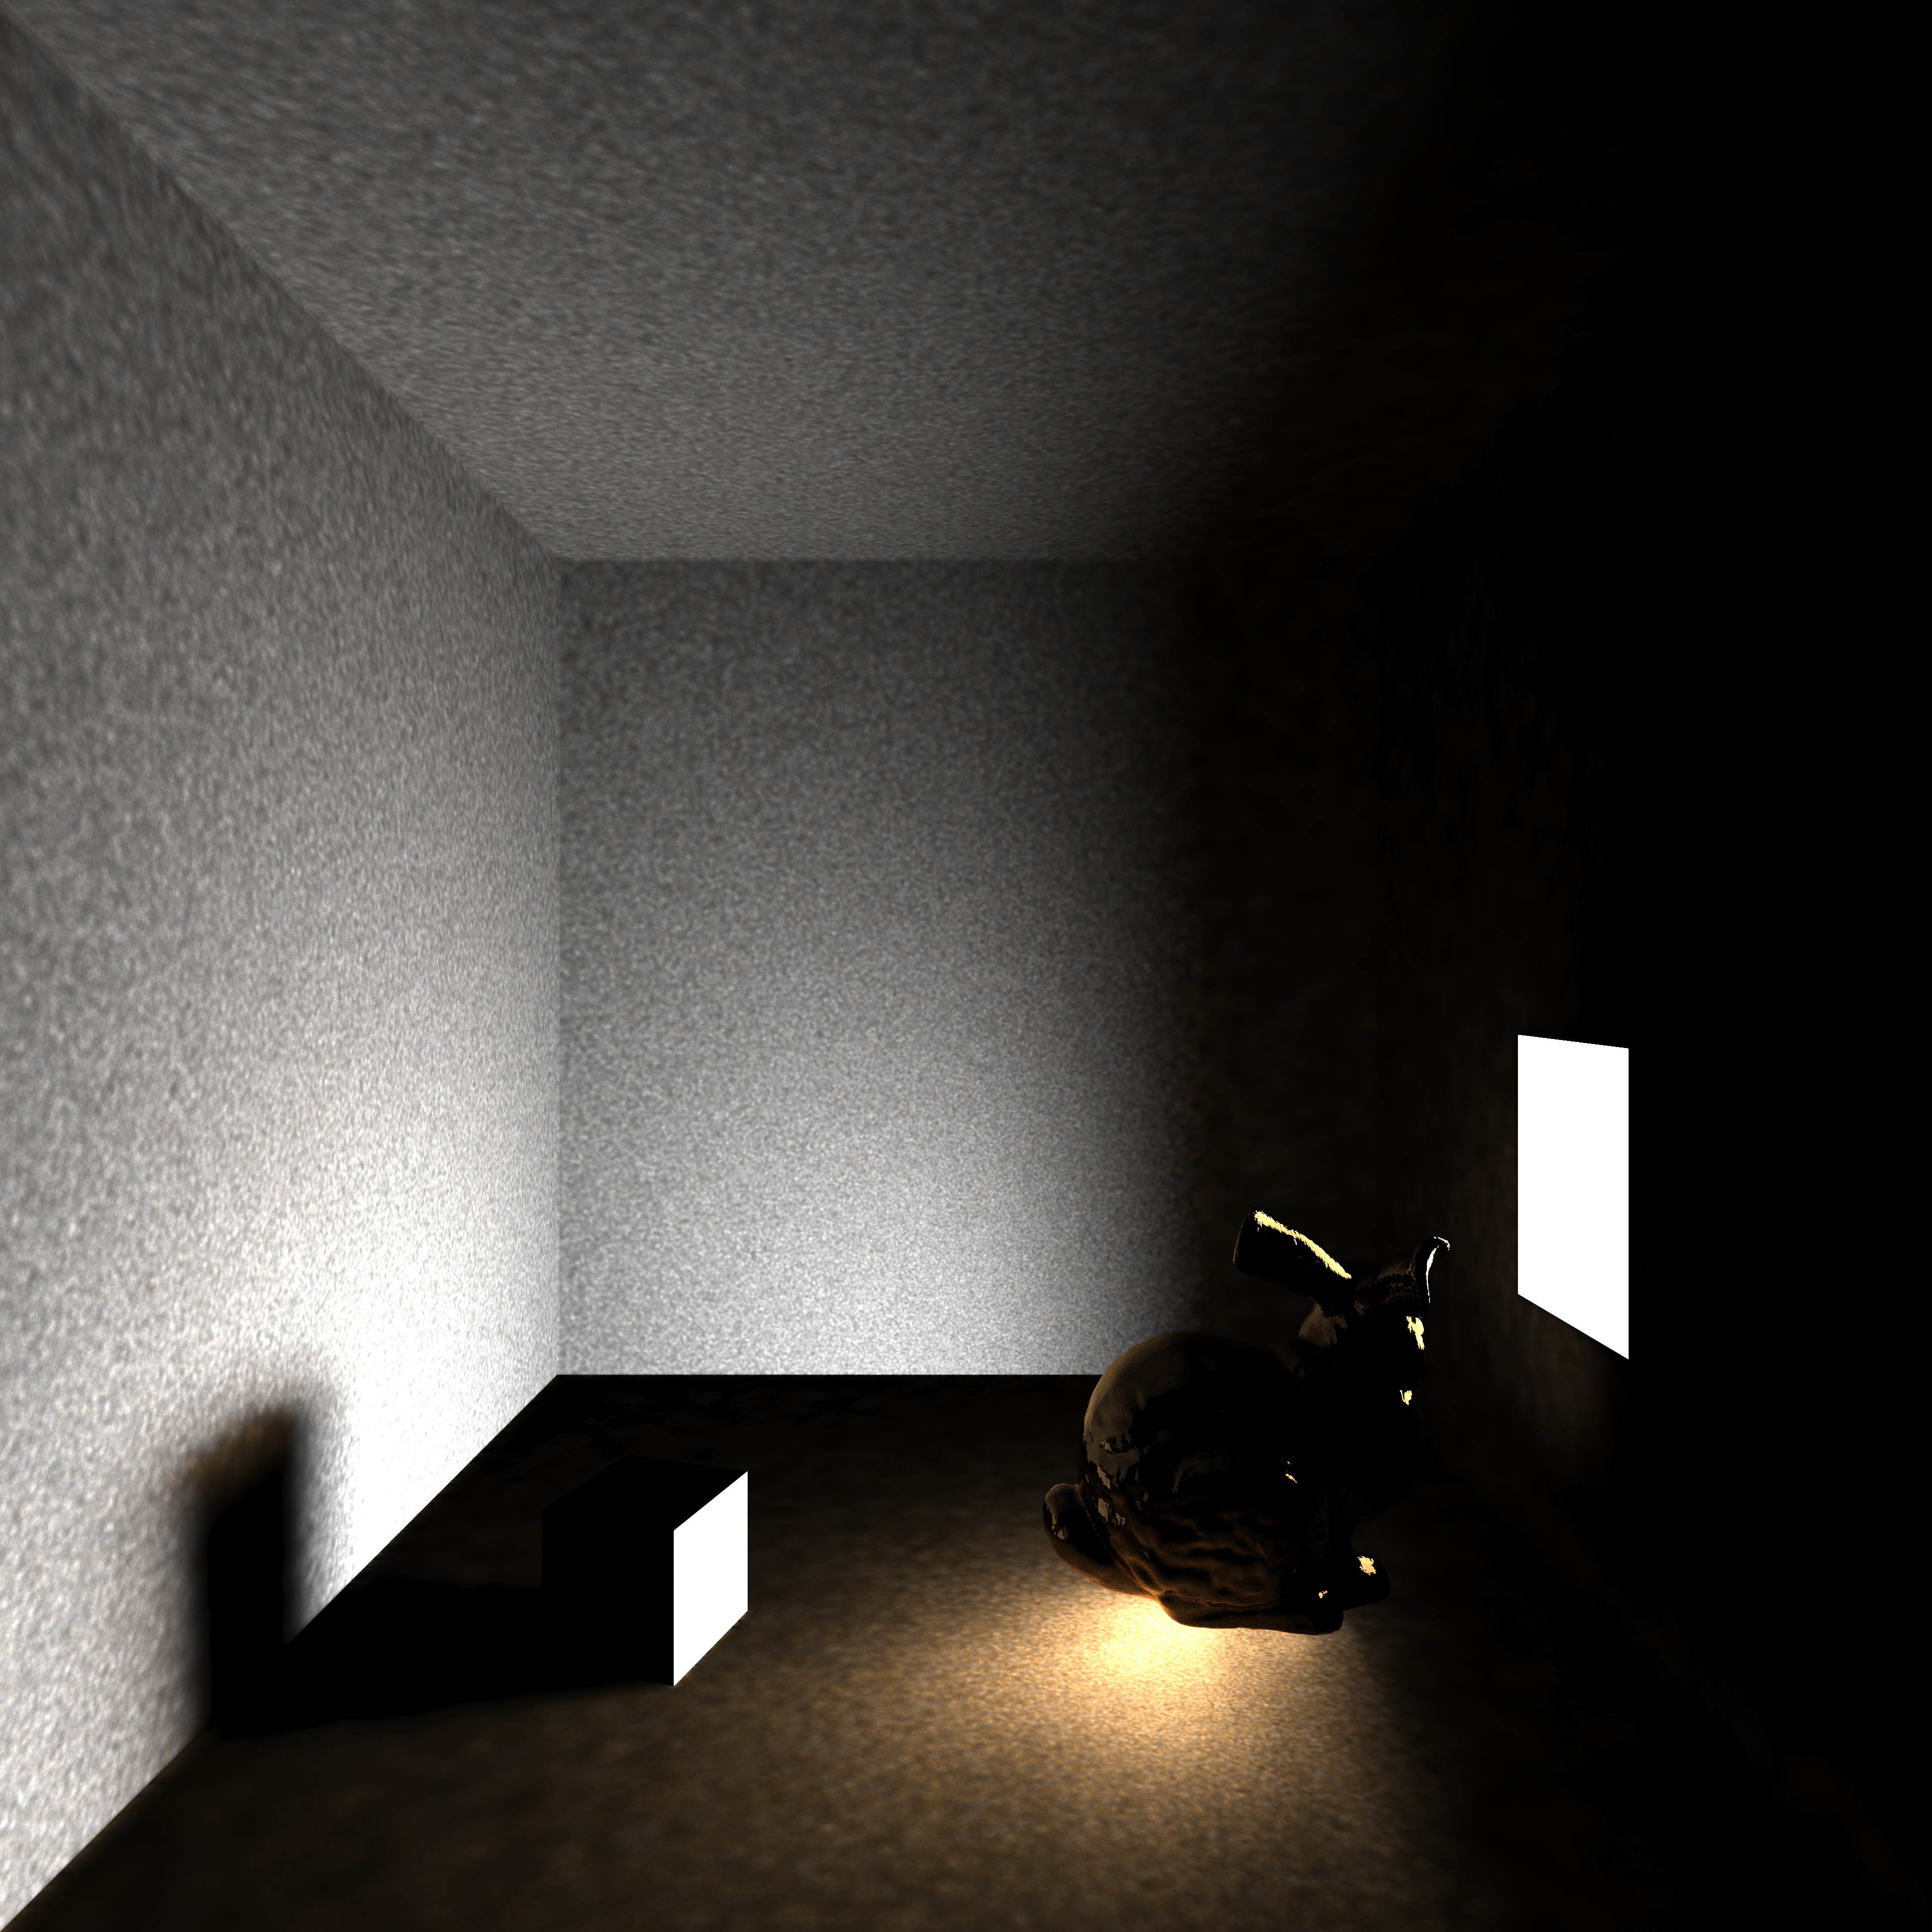
\includegraphics[width=0.5\linewidth]{../_results/photon_mapping_bunny_caustic}
	\caption{Photon Mapping Bunny Caustic}
	\label{fig:photonmappingbunnycaustic}
\end{figure}

\begin{figure}[H]
	\centering
	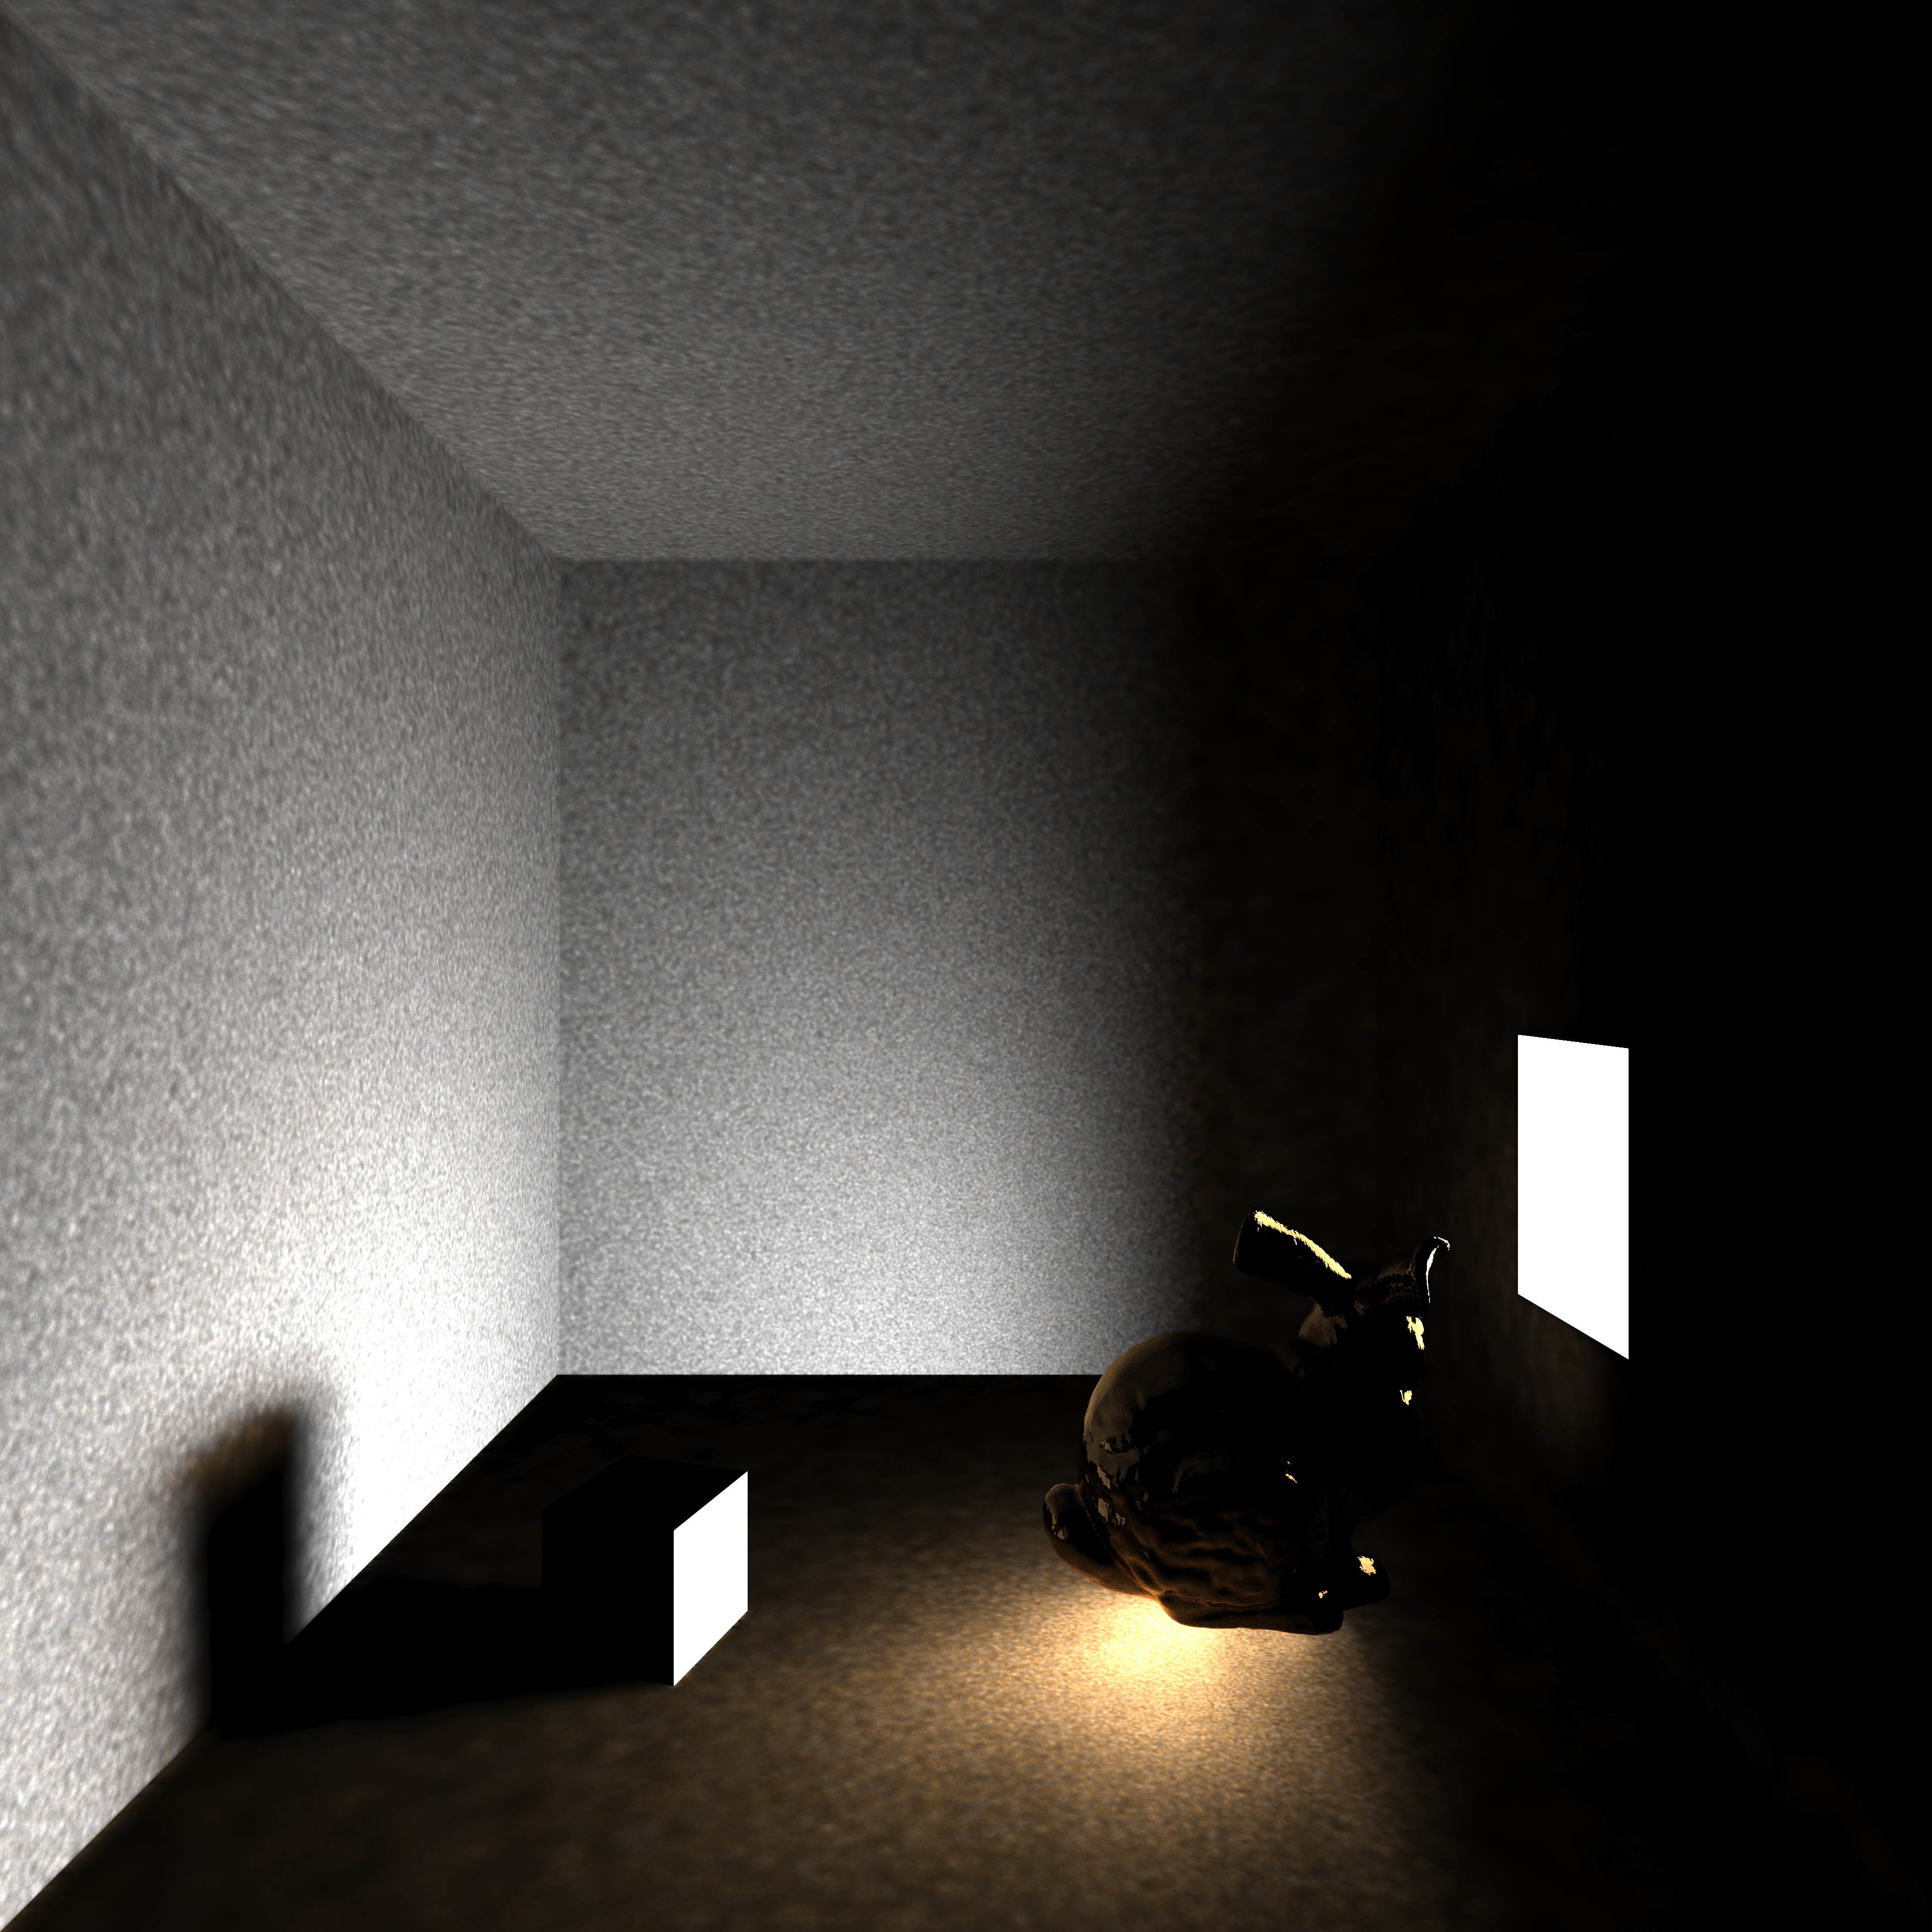
\includegraphics[width=0.5\linewidth]{../_results/photon_mapping_bunny}
	\caption{Photon Mapping Bunny}
	\label{fig:photonmappingbunny}
\end{figure}

\newpage
\section{Usage}

\large \textbf{How to set scene before compilation}

\normalsize
\noindent
\textbf{step 1:} set image settings (customization (e.g. changing aspect$\_$ratio to 16.0 / 9.0) can be done by modifying render$\_$scene in main.cpp)

\noindent
\textbf{step 2:} choose integrator (Photon Mapping only supports one scene, Path Tracing has step 3 of setting scene)

\noindent
\textbf{step 3:} set scene, camera and skybox (scene functions can be found in src/scenes) \\

\noindent
\large \textbf{How to run this renderer}

\normalsize
\noindent
\textbf{Windows:}

\noindent
\textbf{step 1:} compile with CLion using MSVC compiler

\noindent
\textbf{step 2:} run "Project.exe 8", here 8 means using 8 threads (after running we will get 8 .partial files)

\noindent
\textbf{step 3:} run "packager.exe 8", here 8 means combining 8 partial files (after running we will get a .ppm image, which can be opened using OpenSeeIt)

\noindent
\textbf{step 4:} run python convert.py, which converts .ppm into .jpg (note that opencv for python is required to run this)

\noindent
\textbf{Linux:}

run "bash linux$\_$run.sh", which compiles the renderer, uses 80 processes to run it and process result into a .ppm and a .jpg file. (Note that for default Sponza Crytek scene, about 150 GB memory is required. This requirement is proportional to the number of processes.)

\section{Renderer Function Menu}
The basic functionalities of this renderer are listed in this section. Detailed description with code and explanation can be found in the following chapters.

\subsection{Renderer Core:}
\noindent
\textbf{Integrator: } Monte Carlo Path Tracing, Photon Mapping.

\noindent
\textbf{Accelerator: } BVH (AABB with SAH), Kd-Tree.

\noindent
\textbf{Hardware Acceleration: } OpenMP on Windows, Multi-processing on Linux.

\subsection{Objects: }
\noindent
\textbf{Hittable Objects: } Triangle, Triangular Mesh, Box, Sphere.

\noindent
\textbf{Complex Models: } .obj Model with .mtl Material Description.

\noindent
\textbf{Skybox: } Constant Skybox, Directional Skybox, Realistic Skybox, Multi-layer Skybox.

\noindent
\textbf{Transforms: } Rotation, Translation.

\subsection{Materials \& Textures}
\noindent
\textbf{Materials: } Lambertian, Metal, Dielectric, PBR material, Isotropic, Diffuse Light.

\noindent
\textbf{Textures: } Color Texture, Checker Texture, Perlin Noise Texture, Marble Texture, Image Texture, Bump Texture.

\subsection{Visual Effects}
\noindent
\textbf{Camera Effects: } Off-focus Blur, Motion Blur.

\noindent
\textbf{Volumetric Rendering: } Participating Media.

\noindent
\textbf{Other Visual Effects: } Gamma Correction, Caustic.

\section{Renderer Infrastructures}

\subsection{Math Utilities}

\subsubsection{Basic Math Utilities (/src/math/Utils.h)}
\begin{lstlisting}[style=CStyle]
//
// Created by meiyixuan on 2021-12-10.
//

#ifndef PROJECT_UTILS_H
#define PROJECT_UTILS_H

// path
inline std::string model_pth() {
	#if defined(WINDOWS)
	return "./";
	#else
	return "./resources/";
	#endif
}

// memory
using std::shared_ptr;
using std::make_shared;

// statistics
int normal_triangles = 0;
int u_degrade_triangles = 0;
int v_degrade_triangles = 0;
int unrecoverable_triangles = 0;

// integrator
int integrator_type;

int use_photon_map() { return 1; }

int use_path_tracing() { return 0; }

// math
using std::sqrt;
const double inf = std::numeric_limits<double>::infinity();
const double TMIN = 0.001;
const double EPSILON = 0.0000001;
const double pi = 3.1415926535897932385;

inline double deg2rad(double deg) {
	return deg * pi / 180.0;
}

inline double clamp(double x, double min, double max) {
	if (x < min) return min;
	if (x > max) return max;
	return x;
}

// random
inline double random_double_fixed() {
	// random number in [0, 1), with fixed initial seed
	// This function is thread-identical, and should be used in
	// perlin noise and random scene generation.
	return rand() / (RAND_MAX + 1.0);
}

inline double random_double() {
	if (integrator_type == 1) {
		return random_double_fixed();
	}
	// random number in [0, 1)
	static std::random_device rd;
	static std::uniform_real_distribution<double> distribution(0.0, 1.0);
	static std::mt19937 generator(rd());
	return distribution(generator);
}

inline double random_double(double min, double max) {
	// random real in [min,max).
	return min + (max - min) * random_double();
}

inline double random_double_fixed(double min, double max) {
	// random real in [min,max).
	return min + (max - min) * random_double_fixed();
}

inline int random_int_fixed(int min, int max) {
	// Returns a random integer in [min,max].
	return static_cast<int>(random_double_fixed(min, max + 1));
}

// input
int parse_int(const char *buf, size_t len) {
	int res = 0;
	for (size_t i = 0; i < len; ++i) {
		res *= 10;
		res += buf[i] - '0';
	}
	return res;
}

#endif //PROJECT_UTILS_H

\end{lstlisting}
Basic math and random utilities. Note that we need a predictable random function (random$\_$double$\_$fixed) for multiprocessing, since some random number sequences must be identical across processes (e.g. random numbers used in scene initialization). 

\subsubsection{Vector Math (/src/math/Vector3d.h)}
\begin{lstlisting}[style=CStyle]
//
// Created by meiyixuan on 2021-12-09.
// Basic math class for vector operations.
//

#ifndef PROJECT_VECTOR3D_H
#define PROJECT_VECTOR3D_H

class Vector3d {
	public:
	// constructors
	Vector3d() : val{0, 0, 0} {}
	
	Vector3d(double x, double y, double z) : val{x, y, z} {}
	
	// data
	double x() const { return val[0]; }
	
	double y() const { return val[1]; }
	
	double z() const { return val[2]; }
	
	// operators
	Vector3d &operator+=(const Vector3d &v) {
		val[0] += v.val[0];
		val[1] += v.val[1];
		val[2] += v.val[2];
		return *this;
	}
	
	Vector3d &operator-=(const Vector3d &v) {
		val[0] -= v.val[0];
		val[1] -= v.val[1];
		val[2] -= v.val[2];
		return *this;
	}
	
	Vector3d &operator*=(const double t) {
		val[0] *= t;
		val[1] *= t;
		val[2] *= t;
		return *this;
	}
	
	Vector3d &operator/=(const double t) {
		return *this *= 1 / t;
	}
	
	Vector3d operator-() const { return {-val[0], -val[1], -val[2]}; }
	
	double operator[](int i) const { return val[i]; }
	
	double &operator[](int i) { return val[i]; }
	
	double length() const {
		return std::sqrt(squared_length());
	}
	
	double squared_length() const {
		return val[0] * val[0] + val[1] * val[1] + val[2] * val[2];
	}
	
	// utils
	inline static Vector3d random() {
		return {random_double(), random_double(), random_double()};
	}
	
	inline static Vector3d random_fixed() {
		return {random_double_fixed(), random_double_fixed(), random_double_fixed()};
	}
	
	inline static Vector3d random(double min, double max) {
		return {random_double(min, max), random_double(min, max), random_double(min, max)};
	}
	
	inline static Vector3d random_fixed(double min, double max) {
		return {random_double_fixed(min, max), random_double_fixed(min, max), random_double_fixed(min, max)};
	}
	
	bool near_zero() const {
		// Return true if the vector is close to zero in all dimensions.
		const auto s = 1e-8;
		return (fabs(val[0]) < s) && (fabs(val[1]) < s) && (fabs(val[2]) < s);
	}
	
	public:
	
	double val[3];
	
	// for access to val directly
	friend inline std::ostream &operator<<(std::ostream &out, const Vector3d &v);
	
	friend inline Vector3d operator+(const Vector3d &u, const Vector3d &v);
	
	friend inline Vector3d operator-(const Vector3d &u, const Vector3d &v);
	
	friend inline Vector3d operator*(const Vector3d &u, const Vector3d &v);
	
	friend inline Vector3d operator*(double t, const Vector3d &v);
	
	friend inline double dot(const Vector3d &u, const Vector3d &v);
	
	friend inline Vector3d cross(const Vector3d &u, const Vector3d &v);
};

using Point = Vector3d;   // 3D point
using Color = Vector3d;    // RGB color

inline std::ostream &operator<<(std::ostream &out, const Vector3d &v) {
	return out << v.val[0] << ' ' << v.val[1] << ' ' << v.val[2];
}

inline Vector3d operator+(const Vector3d &u, const Vector3d &v) {
	return {u.val[0] + v.val[0], u.val[1] + v.val[1], u.val[2] + v.val[2]};
}

inline Vector3d operator-(const Vector3d &u, const Vector3d &v) {
	return {u.val[0] - v.val[0], u.val[1] - v.val[1], u.val[2] - v.val[2]};
}

inline Vector3d operator*(const Vector3d &u, const Vector3d &v) {
	return {u.val[0] * v.val[0], u.val[1] * v.val[1], u.val[2] * v.val[2]};
}

inline Vector3d operator*(double t, const Vector3d &v) {
	return {t * v.val[0], t * v.val[1], t * v.val[2]};
}

inline Vector3d operator*(const Vector3d &v, double t) {
	return t * v;
}

inline Vector3d operator/(Vector3d v, double t) {
	return (1 / t) * v;
}

inline double dot(const Vector3d &u, const Vector3d &v) {
	return u.val[0] * v.val[0] + u.val[1] * v.val[1] + u.val[2] * v.val[2];
}

inline Vector3d cross(const Vector3d &u, const Vector3d &v) {
	return {u.val[1] * v.val[2] - u.val[2] * v.val[1],
		u.val[2] * v.val[0] - u.val[0] * v.val[2],
		u.val[0] * v.val[1] - u.val[1] * v.val[0]};
}

inline Vector3d normalize(Vector3d v) {
	return v / v.length();
}

Vector3d random_in_unit_disk() {
	while (true) {
		auto p = Vector3d(random_double(-1, 1), random_double(-1, 1), 0);
		if (p.squared_length() >= 1) continue;
		return p;
	}
}

Vector3d random_in_unit_sphere() {
	// uses reject sampling to generate a random point
	while (true) {
		auto p = Vector3d::random(-1, 1);
		if (p.squared_length() >= 1) continue;
		return p;
	}
}

Vector3d random_unit_vector() {
	return normalize(random_in_unit_sphere());
}

Vector3d random_in_hemisphere(const Vector3d &normal) {
	Vector3d in_unit_sphere = random_in_unit_sphere();
	if (dot(in_unit_sphere, normal) > 0.0)
	return in_unit_sphere;
	else
	return -in_unit_sphere;
}

Vector3d reflect(const Vector3d &v, const Vector3d &n) {
	return v - 2 * dot(v, n) * n;
}

Vector3d refract(const Vector3d &uv, const Vector3d &n, double refract_coefficient) {
	// eta: typically air = 1.0, glass = 1.3 - 1.7, diamond = 2.4
	// refract_coefficient is equal to eta_in / eta_out
	auto cos_theta = fmin(dot(-uv, n), 1.0);
	Vector3d r_out_perp = refract_coefficient * (uv + cos_theta * n);
	Vector3d r_out_parallel = -sqrt(fabs(1.0 - r_out_perp.squared_length())) * n;
	return r_out_perp + r_out_parallel;
}

#endif //PROJECT_VECTOR3D_H

\end{lstlisting}
This file contains all we need for vector math. Note that reflection, refraction and random vector sampling are all defined here as well.

\subsubsection{Perlin Noise (/src/math/Perlin.h)}
\begin{lstlisting}[style=CStyle]
//
// Created by meiyixuan on 2021-12-18.
// Perlin noise generator uses code from Peter Shirley.
// Warning: Perlin noise generator must have identical seeds across all processes.
//

#ifndef PROJECT_PERLIN_H
#define PROJECT_PERLIN_H

class PerlinNoise {
	public:
	PerlinNoise() {
		rand_vector = new Vector3d[point_count];
		for (int i = 0; i < point_count; ++i) {
			rand_vector[i] = normalize(Vector3d::random_fixed(-1, 1));
		}
		
		perm_x = perlin_generate_perm();
		perm_y = perlin_generate_perm();
		perm_z = perlin_generate_perm();
	}
	
	~PerlinNoise() {
		delete[] rand_vector;
		delete[] perm_x;
		delete[] perm_y;
		delete[] perm_z;
	}
	
	double turbulence(const Point &p, int sample_depth = 7) const {
		// initialize
		auto sum = 0.0;
		auto cur_point = p;
		auto weight = 1.0;
		
		// weighted sum of samples
		for (int i = 0; i < sample_depth; i++) {
			sum += weight * noise(cur_point);
			weight *= 0.5;
			cur_point *= 2;
		}
		return fabs(sum);
	}
	
	double noise(const Point &p) const {
		// only one sample from perlin noise
		auto u = p.x() - floor(p.x());
		auto v = p.y() - floor(p.y());
		auto w = p.z() - floor(p.z());
		auto i = static_cast<int>(floor(p.x()));
		auto j = static_cast<int>(floor(p.y()));
		auto k = static_cast<int>(floor(p.z()));
		Vector3d c[2][2][2];
		
		for (int di = 0; di < 2; di++)
		for (int dj = 0; dj < 2; dj++)
		for (int dk = 0; dk < 2; dk++)
		c[di][dj][dk] = rand_vector[
		perm_x[(i + di) & 255] ^
		perm_y[(j + dj) & 255] ^
		perm_z[(k + dk) & 255]];
		
		// tri-linear interpolation
		return perlin_interpolation(c, u, v, w);
	}
	
	private:
	static const int point_count = 256;
	Vector3d *rand_vector;
	int *perm_x;
	int *perm_y;
	int *perm_z;
	
	static int *perlin_generate_perm() {
		auto p = new int[point_count];
		for (int i = 0; i < PerlinNoise::point_count; i++)
		p[i] = i;
		permute(p, point_count);
		return p;
	}
	
	static void permute(int *p, int n) {
		for (int i = n - 1; i > 0; i--) {
			int target = random_int_fixed(0, i);
			int tmp = p[i];
			p[i] = p[target];
			p[target] = tmp;
		}
	}
	
	static double perlin_interpolation(Vector3d c[2][2][2], double u, double v, double w) {
		// hermite smoothing to eliminate Mach Band
		auto uu = u * u * (3 - 2 * u);
		auto vv = v * v * (3 - 2 * v);
		auto ww = w * w * (3 - 2 * w);
		
		// interpolate
		auto accum = 0.0;
		for (int i = 0; i < 2; i++)
		for (int j = 0; j < 2; j++)
		for (int k = 0; k < 2; k++) {
			Vector3d weight_v(u - i, v - j, w - k);
			accum += (i * uu + (1 - i) * (1 - uu))
			* (j * vv + (1 - j) * (1 - vv))
			* (k * ww + (1 - k) * (1 - ww))
			* dot(c[i][j][k], weight_v);
		}
		return accum;
	}
};

#endif //PROJECT_PERLIN_H

\end{lstlisting}
This file defines a simple Perlin Noise Generator. Perlin Noise is a technique often used in procedural texture generation. In this project, it is used to generate marble texture.


\subsection{Basic Datatypes}

\subsubsection{Ray (src/core/Ray.h)}
\begin{lstlisting}[style=CStyle]
//
// Created by meiyixuan on 2021-12-09.
// This file contains the definition of Ray.
//

#ifndef PROJECT_RAY_H
#define PROJECT_RAY_H

class Ray {
	public:
	Ray() : o(), d(), tm{} {}
	
	Ray(const Point &origin, const Vector3d &direction, double time = 0.0, bool _is_camera_ray = false) :
	o(origin), d(direction), tm(time), is_camera_ray(_is_camera_ray) {}
	
	// utils
	Point origin() const { return o; }
	
	Vector3d direction() const { return d; }
	
	double time() const { return tm; }
	
	bool camera_ray() const { return is_camera_ray; }
	
	Point at(double t) const { return o + t * d; }
	
	private:
	// origin and direction
	Point o;
	Vector3d d;
	double tm;
	bool is_camera_ray{false};
};


#endif //PROJECT_RAY_H

\end{lstlisting}
This file defines Ray. Each ray has an origin, a direction and a timestamp. The timestamp is used in motion blur. Also, $is\_camera\_ray$ here is used in skybox to separate visual effect from real lighting effect.

\subsubsection{Pixel (src/core/Pixel.h)}
\begin{lstlisting}[style=CStyle]
//
// Created by meiyixuan on 2021-12-09.
// This file contains the definition of Pixel.
//

#ifndef PROJECT_PIXEL_H
#define PROJECT_PIXEL_H

class Pixel {
	public:
	Pixel() : pixel_color(), write_flag(false), sample_count(1) {}
	
	void set(const Color &color, int samples_per_pixel) {
		pixel_color = color;
		sample_count = samples_per_pixel;
	}
	
	Color get_color() const { return pixel_color; }
	
	int get_sample_count() const { return sample_count; }
	
	void write(std::ofstream &out) {
		// a pixel can only be written once for correctness
		if (!write_flag) {
			write_flag = true;
		} else {
			throw std::runtime_error("A pixel is written twice");
		}
		
		// divide by sample count and gamma correct
		auto r = pixel_color.x();
		auto g = pixel_color.y();
		auto b = pixel_color.z();
		auto scale = 1.0 / sample_count;
		r = sqrt(scale * r);
		g = sqrt(scale * g);
		b = sqrt(scale * b);
		
		// scale to [0, 255] and output
		out << static_cast<int>(256 * clamp(r, 0.0, 0.999)) << ' '
		<< static_cast<int>(256 * clamp(g, 0.0, 0.999)) << ' '
		<< static_cast<int>(256 * clamp(b, 0.0, 0.999)) << '\n';
	}
	
	private:
	bool write_flag;
	Color pixel_color;
	int sample_count;
};

#endif //PROJECT_PIXEL_H
\end{lstlisting}
This file defines Pixel, a data structure that is responsible for writing pixel into files. Note that in line 30 - 37 we add a simple Gamma correction to make the image more realistic.

\subsubsection{Hit (src/core/Hit.h)}
\begin{lstlisting}[style=CStyle]
//
// Created by meiyixuan on 2021-12-18.
//

#ifndef PROJECT_HIT_H
#define PROJECT_HIT_H

struct Hit {
	Point hit_point;
	Vector3d normal;
	std::shared_ptr<Material> mat_ptr;
	double t{0};
	double u{0};
	double v{0};
	bool front_face{false};
	// 0: diffuse, 1: reflect, 2: refract, 3: isotropic
	int scatter_mode{-1};
	int remaining_bounce{-1};
	
	inline void set_face_normal(const Ray &r, const Vector3d &n) {
		front_face = (dot(r.direction(), n) < 0);
		normal = front_face ? n : -n;
	}
};

#endif //PROJECT_HIT_H

\end{lstlisting}
This data structure contains everything needed to be stored when a hit happens.

\subsubsection{AABB (src/core/AABB.h)}
\begin{lstlisting}[style=CStyle]
//
// Created by meiyixuan on 2021-12-15.
//

#ifndef PROJECT_AABB_H
#define PROJECT_AABB_H

class AABB {
	public:
	AABB() = default;
	
	AABB(const Point &min, const Point &max) : minimum(min), maximum(max) {}
	
	Point min() const { return minimum; }
	
	Point max() const { return maximum; }
	
	inline bool hit(const Ray &ray, double t_min, double t_max) const {
		// an optimized slab method (Andrew Kensler at Pixar)
		for (int a = 0; a < 3; a++) {
			auto invD = 1.0f / ray.direction()[a];
			auto t0 = (min()[a] - ray.origin()[a]) * invD;
			auto t1 = (max()[a] - ray.origin()[a]) * invD;
			if (invD < 0.0f)
			std::swap(t0, t1);
			t_min = t0 > t_min ? t0 : t_min;
			t_max = t1 < t_max ? t1 : t_max;
			if (t_max <= t_min)
			return false;
		}
		return true;
	}
	
	inline int longest_axis() const {
		Vector3d length = maximum - minimum;
		if (length[0] >= length[1] && length[0] >= length[2])
		return 0;
		else if (length[1] >= length[0] && length[1] >= length[2])
		return 1;
		else
		return 2;
	}
	
	inline double area() const {
		Vector3d length = maximum - minimum;
		return 2 * (length[0] * length[1] +
		length[0] * length[2] +
		length[1] * length[2]);
	}
	
	private:
	// ranges in three directions (i.e. two points in diagonal)
	Point minimum;
	Point maximum;
};

AABB surrounding_box(AABB box0, AABB box1) {
	Point min(fmin(box0.min().x(), box1.min().x()),
	fmin(box0.min().y(), box1.min().y()),
	fmin(box0.min().z(), box1.min().z()));
	
	Point max(fmax(box0.max().x(), box1.max().x()),
	fmax(box0.max().y(), box1.max().y()),
	fmax(box0.max().z(), box1.max().z()));
	
	return {min, max};
}

#endif //PROJECT_AABB_H

\end{lstlisting}
AABB is abbreviation of axis-aligned-bounding-box, which is used in BVH. Here, $area()$ and $longest\_axis()$ are used in SAH (surface area heuristic) to make the BVH more balanced spatially.

\subsubsection{Photon (src/core/Photon.h)}
\begin{lstlisting}[style=CStyle]
//
// Created by meiyixuan on 2021-12-29.
//

#ifndef PROJECT_PHOTON_H
#define PROJECT_PHOTON_H

struct Photon {
	public:
	Photon() = default;
	
	Photon(Vector3d pos, Vector3d dir, Vector3d _power, int _axis = 0)
	: position(pos), direction(dir), power(_power), axis(_axis) {}
	
	public:
	Vector3d position;
	Vector3d direction;
	Vector3d power; // in color
	int axis{0};
};

#endif //PROJECT_PHOTON_H

\end{lstlisting}
This file contains definition of Photon. A photon stores light intensity at given position. It is generated in forward pass (photon map generation) of Photon Mapping and used in backward pass.

\subsubsection{NearestPhotons (src/core/NearestPhotons.h)}
\begin{lstlisting}[style=CStyle]
//
// Created by meiyixuan on 2021-12-29.
//

#ifndef PROJECT_NEARESTPHOTONS_H
#define PROJECT_NEARESTPHOTONS_H

struct NearestPhotons {
	public:
	NearestPhotons() {
		max_photons = 0;
		found_photons = 0;
		heap_full = false;
		dist_square = nullptr;
		photons = nullptr;
	}
	
	~NearestPhotons() {
		delete[] dist_square;
		delete[] photons;
	}
	
	public:
	Vector3d pos;
	int max_photons, found_photons;
	bool heap_full;
	double* dist_square;
	Photon** photons;
};

#endif //PROJECT_NEARESTPHOTONS_H

\end{lstlisting}
NearestPhotons is a data structure that store nearest photons at given position. It is generated from full PhotonMap and used to determine light intensity at a given point on diffuse surface. 

\subsubsection{PhotonMap (src/core/PhotonMap)}
\begin{lstlisting}[style=CStyle]
//
// Created by meiyixuan on 2021-12-29.
//

#ifndef PROJECT_PHOTONMAP_H
#define PROJECT_PHOTONMAP_H

int calculate_median(int start, int end);

class PhotonMap {
	public:
	PhotonMap() {
		max_photon_num = 10000;
		photon_num = 0;
		photon_list = new Photon[10000];
		box_min = Vector3d(10000, 10000, 10000);
		box_max = Vector3d(-10000, -10000, -10000);
	};
	
	explicit PhotonMap(int max) {
		max_photon_num = max;
		photon_num = 0;
		photon_list = new Photon[max];
		box_min = Vector3d(10000, 10000, 10000);
		box_max = Vector3d(-10000, -10000, -10000);
	};
	
	~PhotonMap() = default;
	
	void store(Photon p) {
		if (photon_num >= max_photon_num) return;
		photon_list[photon_num++] = p;
		box_min = Vector3d(fmin(box_min.x(), p.position.x()),
		fmin(box_min.y(), p.position.y()),
		fmin(box_min.z(), p.position.z()));
		box_max = Vector3d(fmax(box_max.x(), p.position.x()),
		fmax(box_max.y(), p.position.y()),
		fmax(box_max.z(), p.position.z()));
	}
	
	static void median_split(Photon *temp, int start, int end, int med, int axis) {
		// heap sort
		int l = start, r = end;
		while (l < r) {
			double key = temp[r].position[axis];
			int i = l - 1, j = r;
			while (true) {
				while (temp[++i].position[axis] < key);
				while (temp[--j].position[axis] > key && j > l);
				if (i >= j) break;
				std::swap(temp[i], temp[j]);
			}
			std::swap(temp[i], temp[r]);
			if (i >= med) r = i - 1;
			if (i <= med) l = i + 1;
		}
	}
	
	void balance() {
		auto *temp = new Photon[photon_num + 1];
		for (int i = 1; i <= photon_num; ++i) {
			temp[i] = photon_list[i];
		}
		balance_segment(temp, 1, 1, photon_num);
		delete[] temp;
	}
	
	void balance_segment(Photon *temp, int index, int start, int end) {
		if (start == end) {
			photon_list[index] = temp[start];
			return;
		}
		int med = calculate_median(start, end);
		int axis;
		if (box_max.x() - box_min.x() > box_max.y() - box_min.y() &&
		box_max.x() - box_min.x() > box_max.z() - box_min.z())
		axis = 0;
		else if (box_max.y() - box_min.y() > box_max.z() - box_min.z())
		axis = 1;
		else
		axis = 2;
		median_split(temp, start, end, med, axis);
		photon_list[index] = temp[med];
		photon_list[index].axis = axis;
		if (start < med) {
			double tmp = box_max[axis];
			box_max[axis] = photon_list[index].position[axis];
			balance_segment(temp, index * 2, start, med - 1);
			box_max[axis] = tmp;
		}
		if (med < end) {
			double tmp = box_min[axis];
			box_min[axis] = photon_list[index].position[axis];
			balance_segment(temp, index * 2 + 1, med + 1, end);
			box_min[axis] = tmp;
		}
	}
	
	void get_nearest_photons(NearestPhotons *nearest_photons, int index) {
		if (index > photon_num) return;
		Photon *photon = &photon_list[index];
		if (index * 2 <= photon_num) {
			double dist = nearest_photons->pos[photon->axis] - photon->position[photon->axis];
			if (dist < 0) {
				get_nearest_photons(nearest_photons, index * 2);
				if (dist * dist < nearest_photons->dist_square[0])
				get_nearest_photons(nearest_photons, index * 2 + 1);
			} else {
				get_nearest_photons(nearest_photons, index * 2 + 1);
				if (dist * dist < nearest_photons->dist_square[0])
				get_nearest_photons(nearest_photons, index * 2);
			}
		}
		double dist_square = (photon->position - nearest_photons->pos).squared_length();
		if (dist_square > nearest_photons->dist_square[0]) return;
		if (nearest_photons->found_photons < nearest_photons->max_photons) {
			nearest_photons->found_photons++;
			nearest_photons->dist_square[nearest_photons->found_photons] = dist_square;
			nearest_photons->photons[nearest_photons->found_photons] = photon;
		} else {
			if (!nearest_photons->heap_full) {
				for (int i = nearest_photons->found_photons >> 1; i >= 1; --i) {
					int par = i;
					auto temp_photon = nearest_photons->photons[i];
					double temp_dist_square = nearest_photons->dist_square[i];
					while ((par << 1) <= nearest_photons->found_photons) {
						int j = par << 1;
						if (j + 1 <= nearest_photons->found_photons
						&& nearest_photons->dist_square[j] < nearest_photons->dist_square[j + 1])
						j++;
						if (temp_dist_square >= nearest_photons->dist_square[j]) break;
						nearest_photons->photons[par] = nearest_photons->photons[j];
						nearest_photons->dist_square[par] = nearest_photons->dist_square[j];
						par = j;
					}
					nearest_photons->photons[par] = temp_photon;
					nearest_photons->dist_square[par] = temp_dist_square;
				}
				nearest_photons->heap_full = true;
			}
			int par = 1;
			while ((par << 1) <= nearest_photons->found_photons) {
				int j = par << 1;
				if (j + 1 <= nearest_photons->found_photons
				&& nearest_photons->dist_square[j] < nearest_photons->dist_square[j + 1])
				j++;
				if (dist_square >= nearest_photons->dist_square[j]) break;
				nearest_photons->photons[par] = nearest_photons->photons[j];
				nearest_photons->dist_square[par] = nearest_photons->dist_square[j];
				par = j;
			}
			nearest_photons->photons[par] = photon;
			nearest_photons->dist_square[par] = dist_square;
			nearest_photons->dist_square[0] = nearest_photons->dist_square[1];
		}
	}
	
	Color get_irradiance(Vector3d pos, Vector3d norm, double max_dist, int N) {
		Vector3d ret(0, 0, 0);
		NearestPhotons np;
		np.pos = pos;
		np.max_photons = N;
		np.dist_square = new double[N + 1];
		np.photons = new Photon *[N + 1];
		np.dist_square[0] = max_dist * max_dist;
		get_nearest_photons(&np, 1);
		if (np.found_photons <= 0.3 * N) return ret;
		for (int i = 1; i <= np.found_photons; ++i) {
			auto dir = np.photons[i]->direction;
			// filtering
			double filter = 1.0 - (pos - np.photons[i]->position).length() / (1.1 * max_dist);
			if (dot(norm, dir) < 0) ret = ret + np.photons[i]->power * filter;
		}
		ret = ret * (1.0 / (500000 * pi * np.dist_square[0]));
		return ret;
	}
	
	int get_photon_num() const { return photon_num; }
	
	private:
	int photon_num;
	int max_photon_num;
	Photon *photon_list;
	Point box_min, box_max;
};

int calculate_median(int start, int end) {
	int num = end - start + 1;
	int med;
	int as = 1, b = 2;
	while (as < num) {
		as += b;
		b *= 2;
	}
	if (as == num) return start + num / 2;
	b /= 2;
	if (as - b / 2 < num) {
		return start + as / 2;
	} else {
		return start + as / 2 - (as - b / 2 - num);
	}
}

#endif //PROJECT_PHOTONMAP_H

\end{lstlisting}
This is really a long file. PhotonMap is a data structure based on balanced Kd-Tree. In building stage, it is responsible for storing all photons generated by the Photon Mapper. In backward tracing stage, it serves as an oracle that returns nearest photons of any given position (as radiance). This part of the code heavily relies on Code Reference [3]'s code with some minor modifications.

\subsection{External Libraries}

\subsubsection{stb$\_$image (ext/stb$\_$image/stb$\_$image$\_$header.h)}
\begin{lstlisting}[style=CStyle]
//
// Created by meiyixuan on 2021-12-18.
// This file imports stb_image.h
//

#ifndef PROJECT_STB_IMAGE_HEADER_H
#define PROJECT_STB_IMAGE_HEADER_H

// Disable pedantic warnings for this external library.
#ifdef _MSC_VER
// Microsoft Visual C++ Compiler
#pragma warning (push, 0)
#endif

#define STB_IMAGE_IMPLEMENTATION

#include "stb_image.h"

// Restore warning levels.
#ifdef _MSC_VER
// Microsoft Visual C++ Compiler
#pragma warning (pop)
#endif

#endif //PROJECT_STB_IMAGE_HEADER_H

\end{lstlisting}
stb$\_$image is a nice header-only library designed for loading various kinds of images. It is used to load image into ImageTexture in the renderer. Here we only show our header, instead of the whole external library (which is thousands of lines in length).

\subsubsection{tinyobjloader (ext/tinyobjloader/tiny$\_$obj$\_$loader$\_$header.h)}
\begin{lstlisting}[style=CStyle]
//
// Created by meiyixuan on 2021-12-20.
//

#ifndef PROJECT_TINY_OBJ_LOADER_HEADER_H
#define PROJECT_TINY_OBJ_LOADER_HEADER_H

#define TINYOBJLOADER_USE_DOUBLE
#define TINYOBJLOADER_IMPLEMENTATION
#define TINYOBJLOADER_USE_MAPBOX_EARCUT

#include "tiny_obj_loader.h"

#endif //PROJECT_TINY_OBJ_LOADER_HEADER_H

\end{lstlisting}
tinyobjloader is a header-only library for .obj import. Here, $TINYOBJLOADER\_USE\_DOUBLE$ is defined since our renderer uses double rather than float for float point storage.

$TINYOBJLOADER\_USE\_MAPBOX\_EARCUT$ is defined since our mesh is triangular mesh and does not support shapes with more than three vertices. Mapbox uses Earcut algorithm to perform robust triangularization. Note that although this algorithm is said to be robust, the real result still contains many degenerated triangles (in uv space) and needs extra preprocessing before using.

\section{Renderer Core}

\subsection{Rendering Procedure}
The rendering procedure is quite straightforward. First, in main.cpp, render workers are spawned according to platform and console arguments. Each render worker is responsible for a few lines of the final image and output its result as a .partial file. Then, packager.exe is called to assemble partial files into a .ppm image. After this step, the rendering result is finally visible. However, a typical 4K .ppm image takes around 150MB of disk space. We use convert.py to convert it into a compressed .jpg image, without losing much information. Detailed code are as follows.

\subsubsection{Renderer (main.cpp) and Packager (packager.cpp)}
\noindent
\textbf{main.cpp: }
\begin{lstlisting}[style=CStyle]
//
// Created by meiyixuan on 2021-12-09.
// This is dev branch.
//
/**************************** Usage ****************************/
//
// Note: If compiled on Windows, flag $WINDOWS$ is automatically set. If compiled
//       on Linux, can use $DEBUG$ to switch between debug run (fast) or normal
//       run (high quality).
//
// How set scene before compile:
// step 1: set image settings (customization (e.g. changing aspect_ratio to
//         16.0 / 9.0) can be done by modifying render_scene in main.cpp)
// step 2: choose integrator (Photon Mapping only supports one scene, Path Tracing has step 3
//         of setting scene)
// step 3: set scene, camera and skybox (scene functions can be found in src/scenes)
//
// How to run this renderer:
// Windows:
// step 1: compile with Clion using MSVC compiler
// step 2: run "Project.exe 8", here 8 means using 8 threads
//         (after running we will get 8 .partial files)
// step 3: run "packager.exe 8", here 8 means combining 8 partial files
//         (after running we will get a .ppm image, which can be opened
//         using OpenSeeIt)
// step 4: run python convert.py, which converts .ppm into .jpg
//         (note that opencv for python is required to run this)
// Linux:
// run "bash linux_run.sh", which compiles the renderer, uses 80 processes
// to run it and process result into a .ppm and a .jpg file. (Note that for
// default SponzaCrytek scene, about 150 GB memory is required. This requirement
// is proportional to the number of processes.)
//
/***************************************************************/
#include "Headers.h"

void render_scene(int current_id, int max_processes, const char *output_file) {
	// Image settings
	#if defined(WINDOWS)
	const auto aspect_ratio = 1.0; // 16.0 / 9.0 or 1.0
	const int image_width = 400; // 3840, 800
	const int image_height = static_cast<int>(image_width / aspect_ratio);
	const int samples_per_pixel = 100; // 1000, 100 (x4 if no global light)
	const int max_depth = 10; // 100, 50
	const int photon_map_size = 500000;
	#elif defined(DEBUG)
	const auto aspect_ratio = 1.0; // 16.0 / 9.0 or 1.0
	const int image_width = 800; // 3840, 800
	const int image_height = static_cast<int>(image_width / aspect_ratio);
	const int samples_per_pixel = 100; // 1000, 100 (x4 if no global light)
	const int max_depth = 10; // 100, 50
	const int photon_map_size = 5000000;
	#else
	const auto aspect_ratio = 1.0; // 16.0 / 9.0 or 1.0
	const int image_width = 3840;
	const int image_height = static_cast<int>(image_width / aspect_ratio);
	const int samples_per_pixel = 1000;
	const int max_depth = 50;
	const int photon_map_size = 20000000;
	#endif
	
	// image
	auto image = std::vector<std::vector<Pixel>>();
	for (int idx = 0; idx < image_height; ++idx) {
		auto row = std::vector<Pixel>(image_width);
		image.push_back(std::move(row));
	}
	
	// multiprocessing related (id = 0 - max_processes - 1)
	int work_load = image_height / max_processes;
	int start_row = image_height - 1 - work_load * current_id;
	int end_row = current_id == max_processes - 1 ? -1 : start_row - work_load;
	
	// Render
	/************************* Integrator *************************/
	// first specify use_photon_map() or use_path_tracing()
	// integrator_type = use_photon_map();
	integrator_type = use_path_tracing();
	/**************************************************************/
	if (integrator_type == 0) {
		// World, camera and skybox
		// 1. Note that motion blur objects should be created with 0.0 - 1.0.
		//    Control motion blur with camera's shutter.
		// 2. use global_light_skybox if no other lights enabled
		/************************** Scene **************************/
		HittableList world = sponza_crytek_scene();
		SimpleCamera cam = sponza_crytek_camera(aspect_ratio);
		auto skybox = sponza_crytek_skybox_cloudy();
		/**********************************************************/
		BVHNode world_bvh(world, cam.shutter_open(), cam.shutter_close());
		
		PathTracingIntegrator integrator(world_bvh, skybox);
		for (int j = start_row; j > end_row; --j) {
			std::cerr << "Scanlines remaining: " << j - end_row << '\n' << std::flush;
			auto start = time(nullptr);
			for (int i = 0; i < image_width; ++i) {
				Color pixel_color(0, 0, 0);
				for (int s = 0; s < samples_per_pixel; ++s) {
					auto u = (i + random_double()) / (image_width - 1);
					auto v = (j + random_double()) / (image_height - 1);
					Ray r = cam.get_ray(u, v);
					pixel_color += integrator.cast_ray(r, max_depth);
				}
				image[j][i].set(pixel_color, samples_per_pixel);
			}
			auto end = time(nullptr);
			std::cerr << "loop time " << end - start << "s\n" << std::flush;
		}
	} else if (integrator_type == 1) {
		// World, camera and skybox
		HittableList world = PM_test_scene();
		auto light = PM_test_light();
		world.add(light);
		SimpleCamera cam = PM_test_camera(aspect_ratio);
		auto skybox = PM_test_skybox();
		BVHNode world_bvh(world, cam.shutter_open(), cam.shutter_close());
		
		// photon map and integrator
		auto photon_map = std::make_shared<PhotonMap>(photon_map_size * 1.2);
		auto integrator = PhotonMappingIntegrator(world, skybox, photon_map);
		
		// generate photon map
		Vector3d origin, direction, power = Vector3d(6, 6, 6);
		double power_scale;
		while (photon_map->get_photon_num() < photon_map_size) {
			if (photon_map->get_photon_num() % 100000 == 0)
			std::cerr << "Finished " << photon_map->get_photon_num() << " photons." << std::endl;
			light->generate_photon(origin, direction, power_scale);
			Ray ray(origin, direction);
			integrator.trace_photon(ray, 10, power_scale * power);
		}
		while (photon_map->get_photon_num() < photon_map_size * 1.2) {
			if (photon_map->get_photon_num() % 50000 == 0)
			std::cerr << "Finished " << photon_map->get_photon_num() << " photons." << std::endl;
			light->generate_photon(origin, direction, power_scale);
			Ray ray(origin, direction);
			integrator.trace_photon_caustic(ray, 10,
			power_scale * power * Vector3d(0.87, 0.49, 0.173) * 12);
		}
		photon_map->balance();
		
		// render
		for (int j = start_row; j > end_row; --j) {
			std::cerr << "Scanlines remaining: " << j - end_row << '\n' << std::flush;
			auto start = time(nullptr);
			for (int i = 0; i < image_width; ++i) {
				Color pixel_color(0, 0, 0);
				for (int s = 0; s < samples_per_pixel; ++s) {
					auto u = (i + random_double()) / (image_width - 1);
					auto v = (j + random_double()) / (image_height - 1);
					Ray r = cam.get_ray(u, v);
					pixel_color += integrator.cast_ray(r, max_depth);
				}
				image[j][i].set(pixel_color, samples_per_pixel);
			}
			auto end = time(nullptr);
			std::cerr << "loop time " << end - start << "s\n" << std::flush;
		}
	}
	
	// output
	std::ofstream file;
	file.open(output_file, std::ios::out | std::ios::trunc);
	if (current_id == 0)
	file << "P3\n" << image_width << ' ' << image_height << "\n255\n";
	for (int j = start_row; j > end_row; --j) {
		for (int i = 0; i < image_width; ++i) {
			image[j][i].write(file);
		}
	}
	file.close();
	std::cerr << "\nDone.\n";
}

int main(int argc, char *argv[]) {
	// parse arguments
	if (argc != 2) {
		std::cerr << "Need to specify process count" << std::endl;
		return 0;
	}
	int max_processes = parse_int(argv[1], strlen(argv[1]));
	std::cerr << "Render will use " << max_processes << " processes." << std::endl;
	
	// launch real renderer
	#if defined(WINDOWS)
	
	if (max_processes == 1) {
		render_scene(0, 1, "1.ppm");
	} else {
		omp_set_num_threads(max_processes);
		#pragma omp parallel for
		for (int thread_idx = 0; thread_idx < max_processes; ++thread_idx) {
			std::string file_name = std::to_string(thread_idx) + ".partial";
			render_scene(thread_idx, max_processes, file_name.c_str());
		}
	}
	
	#else
	
	if (max_processes == 1) {
		render_scene(0, 1, "1.ppm");
	} else {
		std::vector<pid_t> pid_list;
		for (int process_idx = 0; process_idx < max_processes; ++process_idx) {
			std::string file_name = std::to_string(process_idx) + ".partial";
			pid_t pid = fork();
			if (pid != 0) {
				// parent
				pid_list.push_back(pid);
				continue;
			} else {
				// child
				std::cerr << "Worker " << process_idx << " initialized on " << pid << std::endl;
				render_scene(process_idx, max_processes, file_name.c_str());
				return 0;
			}
		}
		for (auto pid: pid_list) {
			waitpid(pid, NULL, 0);
		}
	}
	
	#endif
}
\end{lstlisting}

\noindent
\textbf{packager.cpp: }
\begin{lstlisting}[style=CStyle]
//
// Created by meiyixuan on 2021-12-14.
//

#include "Headers.h"

using namespace std;

int main(int argc, char *argv[]) {
	// check argument count
	if (argc != 2) {
		cout << "Need to specify the number of partial files" << endl;
		return 0;
	}
	int file_count = parse_int(argv[1], strlen(argv[1]));
	
	// open output
	ofstream output;
	output.open("1.ppm", ios::out | ios::trunc);
	
	// parse partial files
	for (int idx = 0; idx < file_count; ++idx) {
		// open input
		ifstream input;
		string input_file_name = to_string(idx) + ".partial";
		input.open(input_file_name.c_str());
		
		// parse
		string line;
		while (getline(input, line)) {
			output << line << "\n";
		}
		
		// clean up
		input.close();
	}
	output.close();
}

\end{lstlisting}

\subsubsection{Other files}
\noindent
\textbf{CMakeList.txt}
\begin{lstlisting}[style=CStyle]
cmake_minimum_required(VERSION 3.19)
project(Project)

set(CMAKE_CXX_STANDARD 14)

IF(WIN32)
add_definitions(-D WINDOWS)
set(CMAKE_CXX_FLAGS "${CMAKE_CXX_FLAGS} /openmp")
ELSE()
add_definitions(-D DEBUG)
set(CMAKE_CXX_FLAGS "${CMAKE_CXX_FLAGS} -std=c++17 -O2 -pthread -fopenmp")
ENDIF()

add_executable(Project main.cpp)
add_executable(packager packager.cpp)

\end{lstlisting}

\noindent
\textbf{linux$\_$run.sh}
\begin{lstlisting}[style=CStyle]
cmake .
make clean
make
./Project 80
rm 1.ppm
rm 1.jpg
./packager 80
rm *.partial
python convert.py
\end{lstlisting}

\noindent
\textbf{converter.py}
\begin{lstlisting}[style=CStyle]
import cv2

i = cv2.imread('1.ppm')
cv2.imwrite('1.jpg', i)

\end{lstlisting}

\subsection{Integrator}
\subsubsection{Base Integrator (src/core/Integrator.h)}
\begin{lstlisting}[style=CStyle]
//
// Created by meiyixuan on 2021-12-15.
//

#ifndef PROJECT_INTEGRATOR_H
#define PROJECT_INTEGRATOR_H

class Integrator {
	public:
	Integrator() = delete;
	
	explicit Integrator(const Accelerator &scene, const Skybox &_skybox)
	: world(scene), skybox(_skybox) {}
	
	virtual Color cast_ray(const Ray &r, int remaining_bounce) const = 0;
	
	protected:
	const Accelerator &world;
	const Skybox &skybox;
};

#endif //PROJECT_INTEGRATOR_H

\end{lstlisting}
This is the base class for all integrators. A integrator integrate light intensity along given light path and returns raw pixel color. $world$ represents the whole scene (usually a BVH node) and $skybox$ is a global (usually uniform) light source. Typical integrators include Path Tracing, Photon Mapping, Progressive Photon Mapping, etc. In this project we only implement the first two.

\subsubsection{Path Tracing Integrator (src/integrator/PathTracingIntegrator.h)}
\begin{lstlisting}[style=CStyle]
//
// Created by meiyixuan on 2021-12-18.
//

#ifndef PROJECT_PATHTRACINGINTEGRATOR_H
#define PROJECT_PATHTRACINGINTEGRATOR_H

class PathTracingIntegrator : Integrator {
	public:
	PathTracingIntegrator() = delete;
	
	explicit PathTracingIntegrator(const Accelerator &scene, const Skybox &skybox)
	: Integrator(scene, skybox) {}
	
	Color cast_ray(const Ray &r, int remaining_bounce) const override {
		Hit hit;
		
		// If we've exceeded the ray bounce limit, no more light is gathered.
		if (remaining_bounce <= 0) return {0, 0, 0};
		hit.remaining_bounce = remaining_bounce;
		
		// If hit nothing, return background
		if (!world.hit(r, TMIN, inf, hit)) return skybox.get_color(r);
		
		// hit something
		Ray scattered_ray;
		Color emit_color = hit.mat_ptr->emit(hit.u, hit.v, hit.hit_point);
		
		// no scattering
		if (!hit.mat_ptr->scatter(r, hit, scattered_ray))
		return emit_color;
		
		// scattering
		Color attenuation = hit.mat_ptr->brdf(r, scattered_ray, hit);
		Color scatter_color = cast_ray(scattered_ray, remaining_bounce - 1);
		return emit_color + attenuation * scatter_color;
	}
};

#endif //PROJECT_PATHTRACINGINTEGRATOR_H

\end{lstlisting}
A Path Tracing integrator reflects and refracts just like normal Ray Tracing integrator. However, when a ray hits a diffuse surface (e.g. Lambertian), instead of sending test rays enumerating lights, path tracing samples a random reflection direction with cos probability and trace the resulting ray. In our implementation, sampling is done in Material. Therefore, Path Tracing Integrator is very short and neat.

\subsubsection{Photon Mapping Integrator (src/integrator/PhotonMappingIntegrator.h)}
\begin{lstlisting}[style=CStyle]
//
// Created by meiyixuan on 2021-12-29.
//

#ifndef PROJECT_PHOTONMAPPINGINTEGRATOR_H
#define PROJECT_PHOTONMAPPINGINTEGRATOR_H

class PhotonMappingIntegrator : public Integrator {
	public:
	PhotonMappingIntegrator(const Accelerator &scene, const Skybox &skybox, std::shared_ptr<PhotonMap> _map)
	: Integrator(scene, skybox), photon_map(std::move(_map)) {}
	
	Color cast_ray(const Ray &r, int remaining_bounce) const override {
		Hit hit;
		if (world.hit(r, TMIN, inf, hit)) {
			Ray scattered_ray;
			Color emit_color = hit.mat_ptr->emit(hit.u, hit.v, hit.hit_point);
			if (remaining_bounce >= 0 && hit.mat_ptr->scatter(r, hit, scattered_ray)) {
				auto attenuation = hit.mat_ptr->brdf(r, scattered_ray, hit);
				Color light_color;
				if (hit.scatter_mode == 0) {
					light_color = photon_map->get_irradiance(hit.hit_point, hit.normal, 0.1, 50);
				} else {
					light_color = cast_ray(scattered_ray, remaining_bounce - 1);
				}
				return emit_color + light_color * attenuation;
			} else {
				return emit_color;
			}
		} else {
			return skybox.get_color(r);
		}
	}
	
	void trace_photon(const Ray &ray, int remaining_bounce, Vector3d power) {
		Hit hit;
		if (world.hit(ray, TMIN, inf, hit)) {
			Ray scattered_ray;
			if (remaining_bounce > 0 && hit.mat_ptr->scatter(ray, hit, scattered_ray)) {
				// store photon at diffuse surface
				if (hit.scatter_mode == 0) {
					photon_map->store(Photon(hit.hit_point, ray.direction(), power));
				}
				// generate a new photon
				Color attenuation = hit.mat_ptr->brdf(ray, scattered_ray, hit);
				trace_photon(scattered_ray, remaining_bounce - 1, power * attenuation);
			}
		}
	}
	
	void trace_photon_caustic(const Ray &ray, int remaining_bounce, Vector3d power) {
		Hit hit;
		if (world.hit(ray, TMIN, inf, hit)) {
			Ray scattered_ray;
			if (remaining_bounce > 0 && hit.mat_ptr->scatter(ray, hit, scattered_ray)) {
				if (hit.scatter_mode == 1 || hit.scatter_mode == 2) {
					trace_photon(scattered_ray, remaining_bounce - 1, power);
				} else {
					if (remaining_bounce == 10) return;
					photon_map->store(Photon(hit.hit_point, ray.direction(), power));
				}
			}
		}
	}
	
	private:
	std::shared_ptr<PhotonMap> photon_map;
};

#endif //PROJECT_PHOTONMAPPINGINTEGRATOR_H

\end{lstlisting}
Photon Mapping is also known as Photon Mapping Path Tracing (PMPT). Different from normal Path Tracing integrators, instead of sampling a random direction at every diffuse surface, it queries a photon map for light intensity information, which gives faster convergence when light is very small. PM has two passes. The first pass is forward path tracing. It sends out rays (i.e. photons) from every light in the scene, let them reflect and refract and store their intensity and position whenever they hit a diffuse surface. Forward ray tracing builds up a photon map (a Kd-tree of <position, intensity> tuples). The second pass is backward path tracing, this pass is identical to normal Path Tracing except that it queries the photon map and uses nearest photons' intensity as light intensity of diffuse hit-point. Note that we need to set a max radius for nearest photon query to prevent points in shadows being lit by faraway photons.

\subsection{Accelerator}
\subsubsection{Base Accelerator (src/core/Accelerator.h)}
\begin{lstlisting}[style=CStyle]
//
// Created by meiyixuan on 2021-12-10.
// This file contains all accelerating data structures.
//

#ifndef PROJECT_ACCELERATOR_H
#define PROJECT_ACCELERATOR_H

using std::shared_ptr;
using std::make_shared;

class Accelerator : public Hittable {
	// Base class for all accelerating data structures
};

#endif //PROJECT_ACCELERATOR_H

\end{lstlisting}
Accelerator, for compatibility, is derived from Hittable.

\subsubsection{Hittable List (src/accelerator/HittableList.h)}
\begin{lstlisting}[style=CStyle]
//
// Created by meiyixuan on 2021-12-18.
//

#ifndef PROJECT_HITTABLELIST_H
#define PROJECT_HITTABLELIST_H

class HittableList : public Accelerator {
	public:
	HittableList() = default;
	
	void clear() { hittable_list.clear(); }
	
	void add(const shared_ptr<Hittable> &obj) { hittable_list.push_back(obj); }
	
	bool hit(const Ray &r, double t_min, double t_max, Hit &hit) const override {
		// initialize
		Hit obj_hit;
		bool has_hit = false;
		auto closest_t = t_max;
		
		// check intersect status
		for (const auto &hittable: hittable_list) {
			if (hittable->hit(r, t_min, closest_t, obj_hit)) {
				has_hit = true;
				closest_t = obj_hit.t;
				hit = obj_hit;
			}
		}
		
		return has_hit;
	}
	
	bool bounding_box(double time0, double time1, AABB &output_box) const override {
		// check if there are objects
		if (hittable_list.empty()) return false;
		
		AABB temp_box;
		bool first_box_flag = true;
		
		for (const auto &object: hittable_list) {
			// if there are infinitely large object, return false
			if (!object->bounding_box(time0, time1, temp_box)) return false;
			
			// check if first box
			output_box = first_box_flag ? temp_box : surrounding_box(output_box, temp_box);
			first_box_flag = false;
		}
		return true;
	}
	
	protected:
	friend class BVHNode;
	
	std::vector<std::shared_ptr<Hittable>> hittable_list;
};

#endif //PROJECT_HITTABLELIST_H

\end{lstlisting}
The simplest form of integrator is a list. Although it has O(n) query complexity, it is still very efficient when objects are not too many and can be used to initialize other accelerators (like BVH).

\subsubsection{BVH (src/accelerator/BVH.h)}
\begin{lstlisting}[style=CStyle]
//
// Created by meiyixuan on 2021-12-18.
//

#ifndef PROJECT_BVH_H
#define PROJECT_BVH_H

class BVHNode : public Accelerator {
	public:
	BVHNode() = default;
	
	BVHNode(HittableList &list, double time0, double time1)
	: BVHNode(list.hittable_list, 0, list.hittable_list.size(), time0, time1) {}
	
	BVHNode(std::vector<shared_ptr<Hittable>> &src_objects, size_t start, size_t end,
	double time0, double time1) {
		// surface-area-heuristic BVH build
		// start inclusive, end exclusive
		
		// special case
		if (src_objects.size() == 1) {
			left = src_objects[0];
			right = nullptr;
			src_objects[0]->bounding_box(time0, time1, box);
			return;
		}
		
		// initialize
		size_t n = end - start;
		std::vector<AABB> boxes = std::vector<AABB>(n);
		std::vector<double> left_area = std::vector<double>(n);
		std::vector<double> right_area = std::vector<double>(n);
		AABB main_box;
		src_objects[start]->bounding_box(time0, time1, main_box);
		for (int i = 1; i < n; ++i) {
			AABB new_box;
			src_objects[start + i]->bounding_box(time0, time1, new_box);
			main_box = surrounding_box(new_box, main_box);
		}
		
		// choose split axis
		int axis = main_box.longest_axis();
		if (axis == 0)
		sort(src_objects.begin() + static_cast<long long>(start),
		src_objects.begin() + static_cast<long long>(end),
		box_x_compare);
		else if (axis == 1)
		sort(src_objects.begin() + static_cast<long long>(start),
		src_objects.begin() + static_cast<long long>(end),
		box_y_compare);
		else
		sort(src_objects.begin() + static_cast<long long>(start),
		src_objects.begin() + static_cast<long long>(end),
		box_z_compare);
		for (int i = 0; i < n; ++i)
		src_objects[start + i]->bounding_box(time0, time1, boxes[i]);
		
		// left area size
		left_area[0] = boxes[0].area();
		AABB left_box = boxes[0];
		for (size_t i = 1; i < n - 1; ++i) {
			left_box = surrounding_box(left_box, boxes[i]);
			left_area[i] = left_box.area();
		}
		
		// right area size
		right_area[n - 1] = boxes[n - 1].area();
		AABB right_box = boxes[n - 1];
		for (size_t i = n - 2; i > 0; --i) {
			right_box = surrounding_box(right_box, boxes[i]);
			right_area[i] = right_box.area();
		}
		
		// use SAH heuristic to find split
		double min_SAH = inf;
		size_t min_SAH_idx;
		for (size_t i = 0; i < n - 1; ++i) {
			double SAH = static_cast<double>(i) * left_area[i] +
			static_cast<double>(n - i - 1) * right_area[i + 1];
			if (SAH < min_SAH) {
				min_SAH_idx = i;
				min_SAH = SAH;
			}
		}
		
		// split
		if (min_SAH_idx == 0)
		left = src_objects[start];
		else
		left = std::make_shared<BVHNode>(src_objects, start, start + min_SAH_idx + 1,
		time0, time1);
		if (min_SAH_idx == n - 2)
		right = src_objects[start + min_SAH_idx + 1];
		else
		right = std::make_shared<BVHNode>(src_objects, start + min_SAH_idx + 1, end,
		time0, time1);
		box = main_box;
	}
	
	bool hit(const Ray &ray, double t_min, double t_max, Hit &hit) const override {
		// if input ray doesn't hit current node
		if (!box.hit(ray, t_min, t_max))
		return false;
		
		// recursively check two child nodes
		bool hit_left = false, hit_right = false;
		if (left) hit_left = left->hit(ray, t_min, t_max, hit);
		if (right) hit_right = right->hit(ray, t_min, hit_left ? hit.t : t_max, hit);
		return hit_left || hit_right;
	}
	
	bool bounding_box(double time0, double time1, AABB &output_box) const override {
		output_box = box;
		return true;
	}
	
	protected:
	// can be either accelerator or object
	shared_ptr<Hittable> left;
	shared_ptr<Hittable> right;
	AABB box;
	
	private:
	static inline bool box_compare(const shared_ptr<Hittable> &a,
	const shared_ptr<Hittable> &b, int axis) {
		AABB box_a;
		AABB box_b;
		
		if (!a->bounding_box(0, 0, box_a) || !b->bounding_box(0, 0, box_b))
		std::cerr << "No bounding box found.\n";
		
		return box_a.min().val[axis] < box_b.min().val[axis];
	}
	
	static inline bool box_x_compare(const shared_ptr<Hittable> &a, const shared_ptr<Hittable> &b) {
		return box_compare(a, b, 0);
	}
	
	static inline bool box_y_compare(const shared_ptr<Hittable> &a, const shared_ptr<Hittable> &b) {
		return box_compare(a, b, 1);
	}
	
	static inline bool box_z_compare(const shared_ptr<Hittable> &a, const shared_ptr<Hittable> &b) {
		return box_compare(a, b, 2);
	}
	
};

#endif //PROJECT_BVH_H

\end{lstlisting}
This file contains a BVH accelerator. It can be initialized using HittableList. Unlike Kd-tree, there is no guarantee for balanced implementation. Therefore, we use surface-area-heuristic (SAH, line 15 - 98) that empirically generates a spatially balanced tree.

\subsubsection{Kd-Tree}
In general, Kd-Tree can also be used in accelerating hit calculation. However, since we have a very fast BVH based on AABB and SAH, we no longer need Kd-Tree for this purpose. Instead, Kd-Tree is used in Photon Map for fast nearest neighbor calculation. For details see 5.2.7.

\subsection{Hardware Acceleration}
\subsubsection*{main.cpp}
\begin{lstlisting}[style=CStyle]
    // launch real renderer
#if defined(WINDOWS)

if (max_processes == 1) {
	render_scene(0, 1, "1.ppm");
} else {
	omp_set_num_threads(max_processes);
	#pragma omp parallel for
	for (int thread_idx = 0; thread_idx < max_processes; ++thread_idx) {
		std::string file_name = std::to_string(thread_idx) + ".partial";
		render_scene(thread_idx, max_processes, file_name.c_str());
	}
}

#else

if (max_processes == 1) {
	render_scene(0, 1, "1.ppm");
} else {
	std::vector<pid_t> pid_list;
	for (int process_idx = 0; process_idx < max_processes; ++process_idx) {
		std::string file_name = std::to_string(process_idx) + ".partial";
		pid_t pid = fork();
		if (pid != 0) {
			// parent
			pid_list.push_back(pid);
			continue;
		} else {
			// child
			std::cerr << "Worker " << process_idx << " initialized on " << pid << std::endl;
			render_scene(process_idx, max_processes, file_name.c_str());
			return 0;
		}
	}
	for (auto pid: pid_list) {
		waitpid(pid, NULL, 0);
	}
}

#endif
\end{lstlisting}
For ray tracing, the most natural way of hardware acceleration is GPU acceleration, especially by using RT cores in NVIDIA GPUs. However, GPU acceleration requires coding with CUDA and managing VRAM, which is more complicated and harder to debug. Therefore, in our implementation we use CPU multi-processing (or multi-threading). This acceleration method is quite straightforward and requires only minor changes to the code (tens of lines).

For Windows platforms, we use OpenMP to spawn multiple render worker threads. By adding only one line, we can achieve almost linear acceleration. However, for Linux based OS, things are a little bit trickier. C++ standard libraries have locks within its implementation (global, thread-wise lock). It will block access from other threads even if all accesses are read accesses. The result is that all cores are busy waiting and no acceleration is achieved. Therefore, for Linux, we use multiprocessing. Render worker processes are forked from main process and gathered after exit. In this way, we can still achieve linear acceleration. For all experiments, we run the renderer with 80 workers on a server with 128 cores and 512GB memory. Hardware acceleration makes things faster about 80x.

\section{Objects}
In this section, we introduce objects defined in our renderer. This ranges from simple shapes to complex model, as well as transforms.

\subsection{Hittable Objects}
\subsubsection{Base Hittable (src/core/Hittable.h)}
\begin{lstlisting}[style=CStyle]
//
// Created by meiyixuan on 2021-12-10.
// This file contains all hittable objects.
//

#ifndef PROJECT_HITTABLE_H
#define PROJECT_HITTABLE_H

// base class for all hittable objects
class Hittable {
	public:
	Hittable() : mat_ptr(nullptr) {}
	
	explicit Hittable(std::shared_ptr<Material> m) : mat_ptr(std::move(m)) {}
	
	virtual bool hit(const Ray &ray, double t_min, double t_max, Hit &hit) const = 0;
	
	virtual bool bounding_box(double time0, double time1, AABB &output_box) const = 0;
	
	protected:
	shared_ptr<Material> mat_ptr;
};

#endif //PROJECT_HITTABLE_H

\end{lstlisting}
All Hittables have two virtual functions to be defined. The first one is $hit$, which determines whether a given ray intersects with the Hittable or not. The second one is $bounding_box$, which returns a proper AABB that surrounds the Hittable. The first one is used by Integrators and the second one by BVH.

\subsubsection{Sphere (src/hittable/Sphere.h)}
\begin{lstlisting}[style=CStyle]
//
// Created by meiyixuan on 2021-12-18.
//

#ifndef PROJECT_SPHERE_H
#define PROJECT_SPHERE_H

class Sphere : public Hittable {
	public:
	// constructors
	Sphere() : r{0} {}
	
	Sphere(Point center, double radius, std::shared_ptr<Material> m) : Hittable(std::move(m)),
	c{center}, r{radius} {};
	
	// utilities
	Point center() const { return c; }
	
	double radius() const { return r; }
	
	bool hit(const Ray &ray, double t_min, double t_max, Hit &hit) const override {
		// calculate
		Vector3d oc = ray.origin() - c;
		auto _a = ray.direction().squared_length();
		auto _b = dot(oc, ray.direction());
		auto _c = oc.squared_length() - r * r;
		auto discriminant = _b * _b - _a * _c;
		if (discriminant < 0) return false;
		auto sqrt_d = sqrt(discriminant);
		
		// fill intersect
		auto root = (-_b - sqrt_d) / _a;
		if (root > t_min && root < t_max) {
			// small root is fine
			hit.t = root;
			hit.hit_point = ray.at(root);
			Vector3d normal = (hit.hit_point - c) / r;
			hit.set_face_normal(ray, normal);
			hit.mat_ptr = mat_ptr;
			get_sphere_uv(normal, hit.u, hit.v);
			return true;
		} else {
			// may use larger root
			root = (-_b + sqrt_d) / _a;
			if (root > t_min && root < t_max) {
				hit.t = root;
				hit.hit_point = ray.at(root);
				Vector3d normal = (hit.hit_point - c) / r;
				hit.set_face_normal(ray, normal);
				hit.mat_ptr = mat_ptr;
				get_sphere_uv(normal, hit.u, hit.v);
				return true;
			} else { return false; }
		}
	}
	
	bool bounding_box(double time0, double time1, AABB &output_box) const override {
		output_box = AABB(c - Vector3d(r, r, r), c + Vector3d(r, r, r));
		return true;
	}
	
	private:
	Point c;
	double r;
	
	static void get_sphere_uv(const Point &outward_normal, double &u, double &v) {
		// outward_normal: a given point on the sphere of radius one, centered at the origin.
		// u: returned value [0,1] of angle around the Y axis from X=-1.
		// v: returned value [0,1] of angle from Y=-1 to Y=+1.
		
		// calculate parameter
		auto theta = acos(-outward_normal.y());
		auto phi = atan2(-outward_normal.z(), outward_normal.x()) + pi;
		
		// calculate uv
		u = phi / (2 * pi);
		v = theta / pi;
	}
};

#endif //PROJECT_SPHERE_H

\end{lstlisting}
The simplest object is a sphere. For $hit$, we use code form Real Time Rendering and Ray Tracing Mini-books.

\subsubsection{Moving Sphere (src/hittable/MovingSphere.h)}
\begin{lstlisting}[style=CStyle]
//
// Created by meiyixuan on 2021-12-18.
//

#ifndef PROJECT_MOVINGSPHERE_H
#define PROJECT_MOVINGSPHERE_H

class MovingSphere : public Hittable {
	public:
	MovingSphere() = default;
	
	MovingSphere(Point cen0, Point cen1, double _time0, double _time1, double r, const shared_ptr<Material> &m)
	: Hittable(m), center0(cen0), center1(cen1), time0(_time0), time1(_time1), radius(r) {};
	
	bool hit(const Ray &ray, double t_min, double t_max, Hit &hit) const override {
		// calculate
		Vector3d oc = ray.origin() - center(ray.time());
		auto _a = ray.direction().squared_length();
		auto _b = dot(oc, ray.direction());
		auto _c = oc.squared_length() - radius * radius;
		auto discriminant = _b * _b - _a * _c;
		if (discriminant < 0) return false;
		auto sqrt_d = sqrt(discriminant);
		
		// fill intersect
		auto root = (-_b - sqrt_d) / _a;
		if (root > t_min && root < t_max) {
			// small root is fine
			hit.t = root;
			hit.hit_point = ray.at(root);
			Vector3d normal = (hit.hit_point - center(ray.time())) / radius;
			hit.set_face_normal(ray, normal);
			hit.mat_ptr = mat_ptr;
			return true;
		} else {
			// may use larger root
			root = (-_b + sqrt_d) / _a;
			if (root > t_min && root < t_max) {
				hit.t = root;
				hit.hit_point = ray.at(root);
				Vector3d normal = (hit.hit_point - center(ray.time())) / radius;
				hit.set_face_normal(ray, normal);
				hit.mat_ptr = mat_ptr;
				return true;
			} else { return false; }
		}
	}
	
	bool bounding_box(double _time0, double _time1, AABB &output_box) const override {
		AABB box0(center(_time0) - Vector3d(radius, radius, radius),
		center(_time0) + Vector3d(radius, radius, radius));
		AABB box1(center(_time1) - Vector3d(radius, radius, radius),
		center(_time1) + Vector3d(radius, radius, radius));
		output_box = surrounding_box(box0, box1);
		return true;
	}
	
	Point center(double time) const {
		return center0 + ((time - time0) / (time1 - time0)) * (center1 - center0);
	}
	
	public:
	Point center0, center1;
	double time0{}, time1{};
	double radius{};
};

#endif //PROJECT_MOVINGSPHERE_H

\end{lstlisting}
Moving spheres have center position as a function of time. Since Rays have time within it, we can use the time to compute the center and reduce it to the problem of checking intersection between static spheres and rays.

\subsubsection{Rectangles (src/hittable/Rectangle.h)}
\begin{lstlisting}[style=CStyle]
//
// Created by meiyixuan on 2021-12-18.
//

#ifndef PROJECT_RECTANGLE_H
#define PROJECT_RECTANGLE_H

class XYRectangle : public Hittable {
	public:
	XYRectangle() = default;
	
	XYRectangle(double _x0, double _x1, double _y0, double _y1, double _z, std::shared_ptr<Material> mat_ptr)
	: Hittable(std::move(mat_ptr)), x0(_x0), x1(_x1), y0(_y0), y1(_y1), z(_z) {}
	
	bool hit(const Ray &ray, double t_min, double t_max, Hit &hit) const override {
		// check if hit plane
		auto t = (z - ray.origin().z()) / ray.direction().z();
		if (t < t_min || t > t_max) return false;
		
		// check if hit rect
		auto x = ray.origin().x() + t * ray.direction().x();
		auto y = ray.origin().y() + t * ray.direction().y();
		if (x < x0 || x > x1 || y < y0 || y > y1) return false;
		
		// hit
		hit.u = (x - x0) / (x1 - x0);
		hit.v = (y - y0) / (y1 - y0);
		hit.t = t;
		auto outward_normal = Vector3d(0, 0, 1);
		hit.set_face_normal(ray, outward_normal);
		hit.mat_ptr = mat_ptr;
		hit.hit_point = ray.at(t);
		return true;
	}
	
	bool bounding_box(double time0, double time1, AABB &output_box) const override {
		output_box = AABB(Point(x0, y0, z - 0.0001), Point(x1, y1, z + 0.0001));
		return true;
	}
	
	private:
	double x0{}, x1{}, y0{}, y1{};
	double z{};
};

class XZRectangle : public Hittable {
	public:
	XZRectangle() = default;
	
	XZRectangle(double _x0, double _x1, double _z0, double _z1, double _y, shared_ptr<Material> mat_ptr)
	: Hittable(std::move(mat_ptr)), x0(_x0), x1(_x1), z0(_z0), z1(_z1), y(_y) {};
	
	bool hit(const Ray &ray, double t_min, double t_max, Hit &hit) const override {
		// check if hit plane
		auto t = (y - ray.origin().y()) / ray.direction().y();
		if (t < t_min || t > t_max) return false;
		
		// check if hit rectangle
		auto x = ray.origin().x() + t * ray.direction().x();
		auto z = ray.origin().z() + t * ray.direction().z();
		if (x < x0 || x > x1 || z < z0 || z > z1) return false;
		
		// hit
		hit.u = (x - x0) / (x1 - x0);
		hit.v = (z - z0) / (z1 - z0);
		hit.t = t;
		auto outward_normal = Vector3d(0, 1, 0);
		hit.set_face_normal(ray, outward_normal);
		hit.mat_ptr = mat_ptr;
		hit.hit_point = ray.at(t);
		return true;
	}
	
	bool bounding_box(double time0, double time1, AABB &output_box) const override {
		output_box = AABB(Point(x0, y - 0.0001, z0), Point(x1, y + 0.0001, z1));
		return true;
	}
	
	private:
	double x0{}, x1{}, z0{}, z1{};
	double y{};
};

class YZRectangle : public Hittable {
	public:
	YZRectangle() = default;
	
	YZRectangle(double _y0, double _y1, double _z0, double _z1, double _x, shared_ptr<Material> mat_ptr)
	: Hittable(std::move(mat_ptr)), y0(_y0), y1(_y1), z0(_z0), z1(_z1), x(_x) {};
	
	bool hit(const Ray &ray, double t_min, double t_max, Hit &hit) const override {
		// check if hit plane
		auto t = (x - ray.origin().x()) / ray.direction().x();
		if (t < t_min || t > t_max) return false;
		
		// check if hit rectangle
		auto y = ray.origin().y() + t * ray.direction().y();
		auto z = ray.origin().z() + t * ray.direction().z();
		if (y < y0 || y > y1 || z < z0 || z > z1) return false;
		
		// hit
		hit.u = (y - y0) / (y1 - y0);
		hit.v = (z - z0) / (z1 - z0);
		hit.t = t;
		auto outward_normal = Vector3d(1, 0, 0);
		hit.set_face_normal(ray, outward_normal);
		hit.mat_ptr = mat_ptr;
		hit.hit_point = ray.at(t);
		return true;
	}
	
	bool bounding_box(double time0, double time1, AABB &output_box) const override {
		output_box = AABB(Point(x - 0.0001, y0, z0), Point(x + 0.0001, y1, z1));
		return true;
	}
	
	private:
	double y0{}, y1{}, z0{}, z1{};
	double x{};
};

#endif //PROJECT_RECTANGLE_H

\end{lstlisting}
We only define axis-aligned rectangles and rely on transforms to generate other ones. Note that we need to ensure that AABB has no zero length edge by setting thickness to a fixed constant, otherwise intersection detection may fail. 

\subsubsection{Box (src/hittable/Box.h)}
\begin{lstlisting}[style=CStyle]
#include <utility>

//
// Created by meiyixuan on 2021-12-18.
//

#ifndef PROJECT_BOX_H
#define PROJECT_BOX_H

class Box : public Hittable {
	public:
	Box() = default;
	
	Box(const Point &p0, const Point &p1, const std::shared_ptr<Material> &mat_ptr) : Hittable(nullptr) {
		// diagonal points
		min_point = p0;
		max_point = p1;
		
		// construct faces
		faces.add(make_shared<XYRectangle>(p0.x(), p1.x(), p0.y(), p1.y(), p1.z(), mat_ptr));
		faces.add(make_shared<XYRectangle>(p0.x(), p1.x(), p0.y(), p1.y(), p0.z(), mat_ptr));
		faces.add(make_shared<XZRectangle>(p0.x(), p1.x(), p0.z(), p1.z(), p1.y(), mat_ptr));
		faces.add(make_shared<XZRectangle>(p0.x(), p1.x(), p0.z(), p1.z(), p0.y(), mat_ptr));
		faces.add(make_shared<YZRectangle>(p0.y(), p1.y(), p0.z(), p1.z(), p1.x(), mat_ptr));
		faces.add(make_shared<YZRectangle>(p0.y(), p1.y(), p0.z(), p1.z(), p0.x(), mat_ptr));
	}
	
	bool hit(const Ray &ray, double t_min, double t_max, Hit &hit) const override {
		return faces.hit(ray, t_min, t_max, hit);
	}
	
	bool bounding_box(double time0, double time1, AABB &output_box) const override {
		output_box = AABB(min_point, max_point);
		return true;
	}
	
	private:
	Point min_point, max_point;
	HittableList faces;
};

#endif //PROJECT_BOX_H

\end{lstlisting}
Box is just six rectangles put together.

\subsubsection{Triangle (src/hittable/Triangle.h)}
\begin{lstlisting}[style=CStyle]
#include <utility>

//
// Created by meiyixuan on 2021-12-20.
//

#ifndef PROJECT_TRIANGLE_H
#define PROJECT_TRIANGLE_H

struct Vertex {
	Vertex(double _u, double _v, Point _point, Vector3d _normal = {0, 0, 0})
	: u(_u), v(_v), point(_point), normal(_normal) {}
	
	double u{0};
	double v{0};
	Point point;
	Vector3d normal;
};

class Triangle : public Hittable {
	public:
	Triangle() = default;
	
	Triangle(std::shared_ptr<Vertex> v0, std::shared_ptr<Vertex> v1, std::shared_ptr<Vertex> v2,
	std::shared_ptr<Material> m, std::shared_ptr<BumpMaterial> b = nullptr)
	: Hittable(std::move(m)), bump_ptr(std::move(b)),
	normal(normalize(cross(v1->point - v0->point, v2->point - v0->point))),
	vertices{std::move(v0), std::move(v1), std::move(v2)} {
		// calculate normal
		if (vertices[0]->normal.length() <= EPSILON &&
		vertices[1]->normal.length() <= EPSILON &&
		vertices[2]->normal.length() <= EPSILON) {
			use_computed_normal = true;
		}
		// calculate uv to xyz map
		map_uv_2_xyz();
	}
	
	bool hit(const Ray &ray, double t_min, double t_max, Hit &hit) const override {
		// initialize (Möller–Trumbore intersection algorithm)
		Vector3d edge1, edge2, h, s, q;
		double a, f, u, v;
		edge1 = vertices[1]->point - vertices[0]->point;
		edge2 = vertices[2]->point - vertices[0]->point;
		h = cross(ray.direction(), edge2);
		a = dot(edge1, h);
		
		// This ray is parallel to this triangle.
		if (a > -EPSILON && a < EPSILON) return false;
		f = 1.0 / a;
		s = ray.origin() - vertices[0]->point;
		u = f * dot(s, h);
		if (u < 0.0 || u > 1.0) return false;
		q = cross(s, edge1);
		v = f * dot(ray.direction(), q);
		if (v < 0.0 || u + v > 1.0) return false;
		
		// At this stage we can compute t to find out where the intersection point is on the line.
		// basic hit information
		double t = f * dot(edge2, q);
		if (t < t_min || t > t_max) return false;
		hit.t = t;
		hit.hit_point = ray.at(t);
		hit.mat_ptr = mat_ptr;
		// set normal
		double w0, w1, w2;
		barycentric(hit.hit_point, w0, w1, w2);
		if (!use_computed_normal)
		hit.normal = normalize(w0 * vertices[0]->normal +
		w1 * vertices[1]->normal +
		w2 * vertices[2]->normal);
		else
		hit.normal = normal;
		// add bump map when available
		if (bump_ptr) {
			// get perturbation
			auto perturb0 = bump_ptr->get_normal(vertices[0]->u, vertices[0]->v);
			auto perturb1 = bump_ptr->get_normal(vertices[1]->u, vertices[1]->v);
			auto perturb2 = bump_ptr->get_normal(vertices[2]->u, vertices[2]->v);
			auto perturb = w0 * perturb0 + w1 * perturb1 + w2 * perturb2;
			hit.normal = normalize(hit.normal + perturb[0] * u_vec + perturb[1] * v_vec);
		}
		hit.set_face_normal(ray, normal);
		// set u v
		hit.u = w0 * vertices[0]->u + w1 * vertices[1]->u + w2 * vertices[2]->u;
		hit.v = w0 * vertices[0]->v + w1 * vertices[1]->v + w2 * vertices[2]->v;
		return true;
	}
	
	bool bounding_box(double time0, double time1, AABB &output_box) const override {
		// x
		double x_min = min3(vertices[0]->point.x(), vertices[1]->point.x(), vertices[2]->point.x());
		double x_max = max3(vertices[0]->point.x(), vertices[1]->point.x(), vertices[2]->point.x());
		if (x_min == x_max) {
			x_min -= 0.0001;
			x_max += 0.0001;
		}
		
		// y
		double y_min = min3(vertices[0]->point.y(), vertices[1]->point.y(), vertices[2]->point.y());
		double y_max = max3(vertices[0]->point.y(), vertices[1]->point.y(), vertices[2]->point.y());
		if (y_min == y_max) {
			y_min -= 0.0001;
			y_max += 0.0001;
		}
		
		// z
		double z_min = min3(vertices[0]->point.z(), vertices[1]->point.z(), vertices[2]->point.z());
		double z_max = max3(vertices[0]->point.z(), vertices[1]->point.z(), vertices[2]->point.z());
		if (z_min == z_max) {
			z_min -= 0.0001;
			z_max += 0.0001;
		}
		
		output_box = AABB({x_min, y_min, z_min}, {x_max, y_max, z_max});
		return true;
	}
	
	private:
	bool use_computed_normal{false};
	Vector3d normal;
	std::shared_ptr<Vertex> vertices[3];
	std::shared_ptr<BumpMaterial> bump_ptr;
	// unit vector of u, v in xyz space
	Vector3d u_vec, v_vec;
	
	inline void barycentric(const Point &p, double &u, double &v, double &w) const {
		// Compute barycentric coordinates (u, v, w) for
		// point p with respect to triangle (0, 1, 2)
		// From Christer Ericson's Real-Time Collision Detection
		Vector3d v0 = vertices[1]->point - vertices[0]->point;
		Vector3d v1 = vertices[2]->point - vertices[0]->point;
		Vector3d v2 = p - vertices[0]->point;
		double d00 = dot(v0, v0);
		double d01 = dot(v0, v1);
		double d11 = dot(v1, v1);
		double d20 = dot(v2, v0);
		double d21 = dot(v2, v1);
		double d = d00 * d11 - d01 * d01;
		v = (d11 * d20 - d01 * d21) / d;
		w = (d00 * d21 - d01 * d20) / d;
		u = 1.0 - v - w;
	}
	
	inline void get_triangle_uv(const Point &p, double &u, double &v) const {
		double a, b, c;
		barycentric(p, a, b, c);
		u = a * vertices[0]->u + b * vertices[1]->u + c * vertices[2]->u;
		v = a * vertices[0]->v + b * vertices[1]->v + c * vertices[2]->v;
	}
	
	inline void map_uv_2_xyz() {
		// 1 wrt 0
		double a1 = vertices[1]->u - vertices[0]->u;
		double a2 = vertices[1]->v - vertices[0]->v;
		Vector3d a_xyz = vertices[1]->point - vertices[0]->point;
		// 2 wrt 0
		double b1 = vertices[2]->u - vertices[0]->u;
		double b2 = vertices[2]->v - vertices[0]->v;
		Vector3d b_xyz = vertices[2]->point - vertices[0]->point;
		// denominator and check for degradation
		double denominator = a1 * b2 - a2 * b1;
		if (fabs(denominator) < EPSILON) {
			bool recover_flag = true;
			// no uv coordinate case
			if (a1 == 0 && a2 == 0 && b1 == 0 && b2 == 0) return;
			// u degradation
			if (vertices[0]->u == vertices[1]->u && vertices[0]->u == vertices[2]->u) {
				double v_min = min3(vertices[0]->v, vertices[1]->v, vertices[2]->v);
				double v_max = max3(vertices[0]->v, vertices[1]->v, vertices[2]->v);
				if (v_min == v_max) recover_flag = false;
				else {
					// we can still recover v in this case
					int max_id = v_max == vertices[0]->v ? 0
					: v_max == vertices[1]->v ? 1 : 2;
					int min_id = v_min == vertices[0]->v ? 0
					: v_min == vertices[1]->v ? 1 : 2;
					double v_scale = 1 / (v_max - v_min);
					v_vec = (vertices[max_id]->point - vertices[min_id]->point) * v_scale;
					u_vec = Vector3d();
					u_degrade_triangles += 1;
					return;
				}
			}
			// v degradation
			if (vertices[0]->v == vertices[1]->v && vertices[0]->v == vertices[2]->v) {
				double u_min = min3(vertices[0]->u, vertices[1]->u, vertices[2]->u);
				double u_max = max3(vertices[0]->u, vertices[1]->u, vertices[2]->u);
				if (u_min == u_max) recover_flag = false;
				else {
					// we can still recover u in this case
					int max_id = u_max == vertices[0]->u ? 0
					: u_max == vertices[1]->u ? 1 : 2;
					int min_id = u_min == vertices[0]->u ? 0
					: u_min == vertices[1]->u ? 1 : 2;
					double u_scale = 1 / (u_max - u_min);
					v_vec = Vector3d();
					u_vec = (vertices[max_id]->point - vertices[min_id]->point) * u_scale;
					v_degrade_triangles += 1;
					return;
				}
			}
			// unable to recover and log
			//            std::cerr << "Failed to map uv to xyz" << std::endl;
			//            if (random_double() < 1) {
				//                std::cerr << vertices[0]->u << "     " << vertices[0]->v << std::endl;
				//                std::cerr << vertices[1]->u << "     " << vertices[1]->v << std::endl;
				//                std::cerr << vertices[1]->u << "     " << vertices[1]->v << std::endl;
				//                std::cerr << std::endl;
				//            }
			u_vec = Vector3d();
			v_vec = Vector3d();
			unrecoverable_triangles += 1;
			return;
		}
		// calculate for u
		double ux = b2 / denominator;
		double uy = -a2 / denominator;
		u_vec = ux * a_xyz + uy * b_xyz;
		// calculate for v
		double vx = -b1 / denominator;
		double vy = a1 / denominator;
		v_vec = vx * a_xyz + vy * b_xyz;
		normal_triangles += 1;
	}
	
	static inline double min3(const double &a, const double &b, const double &c) {
		return fmin(fmin(a, b), c);
	}
	
	static inline double max3(const double &a, const double &b, const double &c) {
		return fmax(fmax(a, b), c);
	}
	
};

#endif //PROJECT_TRIANGLE_H

\end{lstlisting}
Triangle is much more complicated than other Hittable objects, since it need to support triangular mesh. When initialing a Triangle, we need to compute mapping from uv unit vector to xyz vector. This step is essential if we want to use bump map. Note that many triangles may have degenerated uv coordinates (i.e. vertices having identical uv coordinates) and need to be carefully recovered. Also, surface normal is interpolated using barycentric coordinates in $hit$.

\subsubsection{Mesh (src/hittable/Mesh.h)}
\begin{lstlisting}[style=CStyle]
#include <utility>

//
// Created by meiyixuan on 2021-12-20.
//

#ifndef PROJECT_MESH_H
#define PROJECT_MESH_H

class Mesh : public Hittable {
	public:
	Mesh() = default;
	
	explicit Mesh(std::shared_ptr<BVHNode> _mesh) : mesh(std::move(_mesh)) {}
	
	explicit Mesh(HittableList &list, double time0 = 0, double time1 = 1)
	: mesh(std::make_shared<BVHNode>(list, time0, time1)) {}
	
	explicit Mesh(std::vector<shared_ptr<Hittable>> &triangles, double time0 = 0, double time1 = 1)
	: mesh(std::make_shared<BVHNode>(triangles, 0, triangles.size(), time0, time1)) {}
	
	bool hit(const Ray &ray, double t_min, double t_max, Hit &hit) const override {
		return mesh->hit(ray, t_min, t_max, hit);
	}
	
	bool bounding_box(double time0, double time1, AABB &output_box) const override {
		return mesh->bounding_box(time0, time1, output_box);
	}
	
	private:
	std::shared_ptr<BVHNode> mesh;
	
};

#endif //PROJECT_MESH_H

\end{lstlisting}
Mesh is just a BVH of triangles.

\subsubsection{Photon Light (src/hittable/PhotonLight.h)}
\begin{lstlisting}[style=CStyle]
//
// Created by meiyixuan on 2021-12-29.
//

#ifndef PROJECT_PHOTONLIGHT_H
#define PROJECT_PHOTONLIGHT_H

inline Vector3d random_dir(const Vector3d &n);

class YZRectangleLight : public Hittable {
	public:
	YZRectangleLight() = default;
	
	YZRectangleLight(double _y0, double _y1, double _z0, double _z1, double _x, shared_ptr<Material> mat_ptr)
	: Hittable(std::move(mat_ptr)), y0(_y0), y1(_y1), z0(_z0), z1(_z1), x(_x) {};
	
	bool hit(const Ray &ray, double t_min, double t_max, Hit &hit) const override {
		// check if hit plane
		auto t = (x - ray.origin().x()) / ray.direction().x();
		if (t < t_min || t > t_max) return false;
		
		// check if hit rectangle
		auto y = ray.origin().y() + t * ray.direction().y();
		auto z = ray.origin().z() + t * ray.direction().z();
		if (y < y0 || y > y1 || z < z0 || z > z1) return false;
		
		// hit
		hit.u = (y - y0) / (y1 - y0);
		hit.v = (z - z0) / (z1 - z0);
		hit.t = t;
		auto outward_normal = Vector3d(1, 0, 0);
		hit.set_face_normal(ray, outward_normal);
		hit.mat_ptr = mat_ptr;
		hit.hit_point = ray.at(t);
		return true;
	}
	
	bool bounding_box(double time0, double time1, AABB &output_box) const override {
		output_box = AABB(Point(x - 0.0001, y0, z0), Point(x + 0.0001, y1, z1));
		return true;
	}
	
	void generate_photon(Vector3d &origin, Vector3d &direction, double &power) const {
		origin = Vector3d(y0 + random_double_fixed() * (y1 - y0), x, z0 + random_double_fixed() * (z1 - z0));
		direction = random_dir(Vector3d(1, 0, 0));
		power = dot(direction, Vector3d(1, 0, 0));
	}
	
	private:
	double y0{}, y1{}, z0{}, z1{};
	double x{};
};

inline Vector3d random_dir(const Vector3d &n) {
	Vector3d in_unit_sphere;
	while (true) {
		auto p = Vector3d::random_fixed(-1, 1);
		if (p.squared_length() >= 1) continue;
		in_unit_sphere = p;
		break;
	}
	if (dot(in_unit_sphere, n) > 0.0)
	return in_unit_sphere;
	else
	return -in_unit_sphere;
}

#endif //PROJECT_PHOTONLIGHT_H

\end{lstlisting}
Photon Light is derived from normal objects by adding a $generate\_photon$ function. Since we only need YZ Rectangle lights in our scene, this is done in a hard coded way.

\subsection{Complex Models}
\subsubsection*{ObjectParser (src/core/ObjectParser.h)}
\begin{lstlisting}[style=CStyle]
#include <utility>

//
// Created by meiyixuan on 2021-12-20.
//

#ifndef PROJECT_OBJECTPARSER_H
#define PROJECT_OBJECTPARSER_H

class ObjectParser {
	public:
	ObjectParser() = delete;
	
	explicit ObjectParser(std::string _filename, std::string _mtl_path)
	: filename(std::move(_filename)), mtl_path(std::move(_mtl_path)) {}
	
	std::shared_ptr<BVHNode> parse(int bump_map_type = 0, double light_sample_probability = 0,
	Vector3d sun_dir = Vector3d(),
	const std::shared_ptr<Material> &default_material
	= std::make_shared<Lambertian>(Color(1, 1, 1))) {
		// create reader
		tinyobj::ObjReaderConfig reader_config;
		reader_config.mtl_search_path = mtl_path; // Path to material files
		tinyobj::ObjReader reader;
		if (!reader.ParseFromFile(filename, reader_config)) {
			if (!reader.Error().empty()) {
				std::cerr << "TinyObjReader: " << reader.Error();
			}
			exit(1);
		}
		if (!reader.Warning().empty()) {
			std::cout << "TinyObjReader: " << reader.Warning();
		}
		
		// read obj data
		auto &attrib = reader.GetAttrib();
		auto &shapes = reader.GetShapes();
		auto &materials = reader.GetMaterials();
		
		// build material
		std::vector<std::shared_ptr<PBRMaterial>> mat_list;
		std::vector<std::shared_ptr<BumpMaterial>> bump_list;
		for (const auto &mat: materials) {
			mat_list.emplace_back(std::make_shared<PBRMaterial>(mat.name, mtl_path,
			Vector3d(mat.diffuse[0],
			mat.diffuse[1],
			mat.diffuse[2]),
			mat.diffuse_texname,
			Vector3d(mat.specular[0],
			mat.specular[1],
			mat.specular[2]),
			mat.shininess,
			mat.specular_texname,
			Vector3d(mat.emission[0],
			mat.emission[1],
			mat.emission[2]),
			mat.emissive_texname,
			mat.ior,
			Vector3d(mat.transmittance[0],
			mat.transmittance[1],
			mat.transmittance[2]),
			mat.dissolve,
			light_sample_probability,
			sun_dir));
			bump_list.emplace_back(mat.bump_texname.empty() ? nullptr :
			std::make_shared<BumpMaterial>(mtl_path, mat.bump_texname,
			bump_map_type));
		}
		
		// Loop over shapes
		HittableList mesh_list;
		for (const auto &shape: shapes) {
			// initialize storage
			size_t index_offset = 0;
			std::vector<std::shared_ptr<Hittable>> triangles;
			
			// Loop over triangles
			for (size_t f = 0; f < shape.mesh.num_face_vertices.size(); f++) {
				
				// check vertex count
				auto fv = size_t(shape.mesh.num_face_vertices[f]);
				if (fv != 3) {
					std::cerr << "A triangle has " << fv << " vertices." << std::endl;
					index_offset += fv;
					continue;
				}
				
				// construct vertices
				std::vector<std::shared_ptr<Vertex>> vertex_list;
				for (size_t v_id = 0; v_id < fv; v_id++) {
					// access to vertex
					tinyobj::index_t idx = shape.mesh.indices[index_offset + v_id];
					tinyobj::real_t vx = attrib.vertices[3 * size_t(idx.vertex_index) + 0];
					tinyobj::real_t vy = attrib.vertices[3 * size_t(idx.vertex_index) + 1];
					tinyobj::real_t vz = attrib.vertices[3 * size_t(idx.vertex_index) + 2];
					Point point(vx, vy, vz);
					
					// Check if `normal_index` is zero or positive. negative = no normal data
					Vector3d normal;
					if (idx.normal_index >= 0) {
						tinyobj::real_t nx = attrib.normals[3 * size_t(idx.normal_index) + 0];
						tinyobj::real_t ny = attrib.normals[3 * size_t(idx.normal_index) + 1];
						tinyobj::real_t nz = attrib.normals[3 * size_t(idx.normal_index) + 2];
						normal = Vector3d(nx, ny, nz);
					}
					
					// Check if `texcoord_index` is zero or positive. negative = no texcoord data
					double u = 0, v = 0;
					if (idx.texcoord_index >= 0) {
						tinyobj::real_t tx = attrib.texcoords[2 * size_t(idx.texcoord_index) + 0];
						tinyobj::real_t ty = attrib.texcoords[2 * size_t(idx.texcoord_index) + 1];
						u = tx;
						v = ty;
					}
					
					// emplace vertex
					vertex_list.emplace_back(std::make_shared<Vertex>(u, v, point, normal));
				}
				index_offset += fv;
				
				// per-face material (set to Lambertian for debug)
				// shape.mesh.material_ids[f];
				auto mat_id = shape.mesh.material_ids[f];
				auto mat_ptr = mat_id == -1 ? default_material : mat_list[mat_id];
				auto bump_ptr = mat_id == -1 ? nullptr : bump_list[shape.mesh.material_ids[f]];
				
				// create triangle
				auto triangle_ptr = std::make_shared<Triangle>(vertex_list[0], vertex_list[1],
				vertex_list[2], mat_ptr, bump_ptr);
				triangles.push_back(triangle_ptr);
			}
			
			// build mesh
			auto mesh = std::make_shared<Mesh>(triangles);
			mesh_list.add(mesh);
		}
		
		// output parse statistics
		std::cerr << "*********************Parser Statistics*********************" << std::endl;
		std::cerr << "UV Mapping:" << std::endl;
		std::cerr << "Normal: " << normal_triangles << std::endl;
		std::cerr << "U-degrade: " << u_degrade_triangles << std::endl;
		std::cerr << "V-degrade: " << v_degrade_triangles << std::endl;
		std::cerr << "Unrecoverable: " << unrecoverable_triangles << std::endl;
		std::cerr << "***********************************************************" << std::endl;
		
		return std::make_shared<BVHNode>(mesh_list, 0.0, 1.0);
	}
	
	private:
	std::string filename;
	std::string mtl_path;
};

#endif //PROJECT_OBJECTPARSER_H

\end{lstlisting}
For importing complex models, we use tinyobjloader. It can resolve .obj into three separate lists of vertices, normals and uv coordinates. If the model has a .mtl file that contain material description, tinyobjloader can resolve that into a list of parameters as well. In ObjectParser, we first use material parameters to build a list of PBRMaterials (will be explained in section 8) and then enumerate through all shapes, faces and vertices to build up model mesh.

\subsection{Skybox}
\subsubsection{Base Skybox (src/core/Skybox.h)}
\begin{lstlisting}[style=CStyle]
//
// Created by meiyixuan on 2021-12-18.
//

#ifndef PROJECT_SKYBOX_H
#define PROJECT_SKYBOX_H

class Skybox {
	public:
	virtual Color get_color(Ray r) const = 0;
};

#endif //PROJECT_SKYBOX_H

\end{lstlisting}
Rigorously speaking, Skybox is not a hittable object, since it is not derived from Hittable. However, when a ray misses all Hittables in the scene, it automatically collides with the skybox. In this sense, we can view skyboxes as hittables. A skybox takes in a ray and returns color along the ray's direction.

\subsubsection{Constant Skybox (src/skybox/ConstantSkybox.h)}
\begin{lstlisting}[style=CStyle]
//
// Created by meiyixuan on 2021-12-18.
//

#ifndef PROJECT_CONSTANTSKYBOX_H
#define PROJECT_CONSTANTSKYBOX_H

class ConstantSkybox : public Skybox {
	public:
	ConstantSkybox() = default;
	
	explicit ConstantSkybox(Color _sky_color) : sky_color(_sky_color) {}
	
	Color get_color(Ray r) const override {
		return sky_color;
	}
	
	private:
	Color sky_color;
};

#endif //PROJECT_CONSTANTSKYBOX_H

\end{lstlisting}
A skybox that returns constant color.

\subsubsection{Directional Skybox (src/skybox/DirectionalSkybox.h)}
\begin{lstlisting} [style=CStyle]
//
// Created by meiyixuan on 2021-12-23.
//

#ifndef PROJECT_DIRECTIONALSKYBOX_H
#define PROJECT_DIRECTIONALSKYBOX_H

class DirectionalSkybox : public Skybox {
	public:
	DirectionalSkybox() = default;
	
	DirectionalSkybox(double _sky_intensity, double _sun_intensity, Vector3d _dir2sun, double _radius)
	: sky_intensity(_sky_intensity), sun_intensity(_sun_intensity),
	dir2sun(normalize(_dir2sun)), sun_radius(_radius) {}
	
	Color get_color(Ray r) const override {
		if (pow(fmax(dot(normalize(r.direction()), dir2sun), 0), 3) > sun_radius)
		return sun_intensity * Color(1, 1, 1);
		else
		return sky_intensity * Color(0.5, 0.7, 1.0);
	}
	
	private:
	double sky_intensity{1};
	double sun_intensity{3};
	Vector3d dir2sun;
	double sun_radius{0.6};
};

#endif //PROJECT_DIRECTIONALSKYBOX_H

\end{lstlisting}
A skybox that simulates sun effect (sun with no atmosphere refraction). Maybe used as a component in TwoLayerSkybox.

\subsubsection{Simple Skybox (src/skybox/SimpleSkybox.h)}
\begin{lstlisting} [style=CStyle]
//
// Created by meiyixuan on 2021-12-18.
//

#ifndef PROJECT_SIMPLESKYBOX_H
#define PROJECT_SIMPLESKYBOX_H

class SimpleSkybox : public Skybox {
	public:
	SimpleSkybox() = default;
	
	explicit SimpleSkybox(double _intensity) : intensity(_intensity) {}
	
	Color get_color(Ray r) const override {
		Vector3d unit_direction = normalize(r.direction());
		auto t = 0.5 * (unit_direction.y() + 1.0);
		return ((1.0 - t) * Color(1.0, 1.0, 1.0) + t * Color(0.5, 0.7, 1.0))
		* intensity;
	}
	
	private:
	double intensity{1};
};

#endif //PROJECT_SIMPLESKYBOX_H

\end{lstlisting}
A skybox that gradually changes from blue to white from top to bottom.

\subsubsection{Two Layer Skybox (src/skybox/TwoLayerSkybox.h)}
\begin{lstlisting} [style=CStyle]
//
// Created by meiyixuan on 2021-12-28.
//

#ifndef PROJECT_TWOLAYERSKYBOX_H
#define PROJECT_TWOLAYERSKYBOX_H

class TwoLayerSkybox : public Skybox {
	public:
	TwoLayerSkybox() = default;
	
	TwoLayerSkybox(std::shared_ptr<Skybox> visual, std::shared_ptr<Skybox> GI)
	: visual_sky(std::move(visual)), GI_sky(std::move(GI)) {}
	
	Color get_color(Ray r) const override {
		if (r.camera_ray()) {
			return visual_sky->get_color(r);
		} else {
			return GI_sky->get_color(r);
		}
	}
	
	private:
	std::shared_ptr<Skybox> visual_sky;
	std::shared_ptr<Skybox> GI_sky;
};

#endif //PROJECT_TWOLAYERSKYBOX_H

\end{lstlisting}
A skybox that separates visual effect (i.e. rays that directly hit the skybox) from GI effect.

\subsection{Transforms}
In ray tracing, for transforms, we generally do not modify real object position. Instead, we modify ray reversely and use the modified ray to do intersection. This method is equivalent to modifying position directly.

\subsubsection{Base Transform (src/core/Transform.h)}
\begin{lstlisting} [style=CStyle]
//
// Created by meiyixuan on 2021-12-19.
//

#ifndef PROJECT_TRANSFORM_H
#define PROJECT_TRANSFORM_H

class Transform : public Hittable {
};

#endif //PROJECT_TRANSFORM_H

\end{lstlisting}
Base class for transforms, derived from Hittable.

\subsubsection{Translate (src/transform/Translate.h)}
\begin{lstlisting} [style=CStyle]
#include <utility>

//
// Created by meiyixuan on 2021-12-19.
//

#ifndef PROJECT_TRANSLATE_H
#define PROJECT_TRANSLATE_H

class Translate : public Transform {
	public:
	Translate(std::shared_ptr<Hittable> obj, const Vector3d &_displacement)
	: obj_ptr(std::move(obj)), displacement(_displacement) {}
	
	bool hit(const Ray &ray, double t_min, double t_max, Hit &hit) const override {
		// transform
		Ray transformed_ray(ray.origin() - displacement, ray.direction(), ray.time());
		
		// miss
		if (!obj_ptr->hit(transformed_ray, t_min, t_max, hit))
		return false;
		
		// hit
		hit.hit_point += displacement;
		hit.set_face_normal(transformed_ray, hit.normal);
		
		return true;
	}
	
	bool bounding_box(double time0, double time1, AABB &output_box) const override {
		// inf object
		if (!obj_ptr->bounding_box(time0, time1, output_box)) return false;
		
		// normal
		output_box = AABB(output_box.min() + displacement,
		output_box.max() + displacement);
		return true;
	}
	
	private:
	std::shared_ptr<Hittable> obj_ptr;
	Vector3d displacement;
};

#endif //PROJECT_TRANSLATE_H

\end{lstlisting}
Translation moves the origin of target ray by $-displacement$.

\subsubsection{Rotation (src/transform/RotateY.h)}
\begin{lstlisting} [style=CStyle]
#include <utility>

//
// Created by meiyixuan on 2021-12-19.
//

#ifndef PROJECT_ROTATEY_H
#define PROJECT_ROTATEY_H

class RotateY : public Hittable {
	public:
	RotateY(std::shared_ptr<Hittable> p, double angle) : obj_ptr(std::move(p)) {
		auto radians = deg2rad(angle);
		sin_theta = sin(radians);
		cos_theta = cos(radians);
		has_box = obj_ptr->bounding_box(0, 1, transformed_aabb);
		
		Point min(inf, inf, inf);
		Point max(-inf, -inf, -inf);
		
		for (int i = 0; i < 2; i++) {
			for (int j = 0; j < 2; j++) {
				for (int k = 0; k < 2; k++) {
					auto x = i * transformed_aabb.max().x() + (1 - i) * transformed_aabb.min().x();
					auto y = j * transformed_aabb.max().y() + (1 - j) * transformed_aabb.min().y();
					auto z = k * transformed_aabb.max().z() + (1 - k) * transformed_aabb.min().z();
					auto new_x = cos_theta * x + sin_theta * z;
					auto new_z = -sin_theta * x + cos_theta * z;
					Vector3d tester(new_x, y, new_z);
					for (int c = 0; c < 3; c++) {
						min[c] = fmin(min[c], tester[c]);
						max[c] = fmax(max[c], tester[c]);
					}
				}
			}
		}
		transformed_aabb = AABB(min, max);
	}
	
	bool hit(const Ray &ray, double t_min, double t_max, Hit &hit) const override {
		// generate transformed ray
		auto origin = ray.origin();
		auto direction = ray.direction();
		origin[0] = cos_theta * ray.origin()[0] - sin_theta * ray.origin()[2];
		origin[2] = sin_theta * ray.origin()[0] + cos_theta * ray.origin()[2];
		direction[0] = cos_theta * ray.direction()[0] - sin_theta * ray.direction()[2];
		direction[2] = sin_theta * ray.direction()[0] + cos_theta * ray.direction()[2];
		Ray transformed_ray(origin, direction, ray.time());
		
		// miss
		if (!obj_ptr->hit(transformed_ray, t_min, t_max, hit)) return false;
		
		// hit
		auto p = hit.hit_point;
		auto normal = hit.normal;
		p[0] = cos_theta * hit.hit_point[0] + sin_theta * hit.hit_point[2];
		p[2] = -sin_theta * hit.hit_point[0] + cos_theta * hit.hit_point[2];
		normal[0] = cos_theta * hit.normal[0] + sin_theta * hit.normal[2];
		normal[2] = -sin_theta * hit.normal[0] + cos_theta * hit.normal[2];
		hit.hit_point = p;
		hit.set_face_normal(transformed_ray, normal);
		
		return true;
	}
	
	bool bounding_box(double time0, double time1, AABB &output_box) const override {
		output_box = transformed_aabb;
		return has_box;
	}
	
	private:
	std::shared_ptr<Hittable> obj_ptr;
	double sin_theta{0}, cos_theta{1};
	bool has_box;
	AABB transformed_aabb;
};

#endif //PROJECT_ROTATEY_H

\end{lstlisting}
We does not implement general rotation using matrix multiplication. Instead, we only implement around axis rotation, using code similar to that of Ray Tracing Mini-books.

\section{Materials $\&$ Textures}
\subsection{Materials}
\subsubsection{Base Material (src/core/Material.h)}
\begin{lstlisting} [style=CStyle]
//
// Created by meiyixuan on 2021-12-11.
//

#ifndef PROJECT_MATERIAL_H
#define PROJECT_MATERIAL_H

class Hit;

class Material {
	public:
	virtual bool scatter(const Ray &ray_in, Hit &hit, Ray &scattered_ray) const = 0;
	
	virtual Color brdf(const Ray &ray_in, const Ray &ray_out, const Hit &hit) const = 0;
	
	virtual Color emit(double u, double v, const Point &p) const {
		return {0, 0, 0};
	};
	
};

#endif //PROJECT_MATERIAL_H

\end{lstlisting}
This is base class for materials. Every material has a $scatter$ function that computes scattered rays (i.e. reflection, refraction, etc.), a $brdf$ function that computes its response to illumination and a $emit$ function that computes self-emission.

\subsubsection{Lambertian (src/material/Lambertian.h)}
\begin{lstlisting} [style=CStyle]
//
// Created by meiyixuan on 2021-12-18.
//

#ifndef PROJECT_LAMBERTIAN_H
#define PROJECT_LAMBERTIAN_H

class Lambertian : public Material {
	public:
	explicit Lambertian(const Color &a) : albedo(std::make_shared<ColorTexture>(a)) {}
	
	explicit Lambertian(std::shared_ptr<Texture> a) : albedo(std::move(a)) {}
	
	bool scatter(const Ray &ray_in, Hit &hit, Ray &scattered_ray) const override {
		// get scatter direction
		auto scatter_direction = hit.normal + random_unit_vector();
		if (scatter_direction.near_zero())
		scatter_direction = hit.normal;
		
		// generate scattered rays
		scattered_ray = Ray(hit.hit_point, scatter_direction, ray_in.time());
		hit.scatter_mode = 0;
		return true;
	}
	
	Color brdf(const Ray &ray_in, const Ray &ray_out, const Hit &hit) const override {
		return albedo->uv_color(hit.u, hit.v, hit.hit_point);
	}
	
	private:
	std::shared_ptr<Texture> albedo;
};

#endif //PROJECT_LAMBERTIAN_H

\end{lstlisting}
Lambertian is a material that simulate matte, i.e. complete diffuse surface. It scatter rays with direction that follows cos probability distribution. The BRDF function is just the material's albedo.

\subsubsection{Metal (src/material/Metal.h)}
\begin{lstlisting} [style=CStyle]
#include <utility>

//
// Created by meiyixuan on 2021-12-18.
//

#ifndef PROJECT_METAL_H
#define PROJECT_METAL_H

class Metal : public Material {
	public:
	Metal(const Color &a, double f) : albedo(std::make_shared<ColorTexture>(a)), fuzz(f < 1 ? f : 1) {}
	
	Metal(std::shared_ptr<Texture> a, double f) : albedo(std::move(a)), fuzz(f < 1 ? f : 1) {}
	
	bool scatter(const Ray &ray_in, Hit &hit, Ray &scattered_ray) const override {
		// get reflected direction (include perturbation for imperfect reflection)
		Vector3d reflected_dir = reflect(normalize(ray_in.direction()), hit.normal);
		reflected_dir += fuzz * random_in_unit_sphere();
		
		// generate rays
		scattered_ray = Ray(hit.hit_point, reflected_dir, ray_in.time());
		hit.scatter_mode = 1;
		return (dot(reflected_dir, hit.normal) > 0);
	}
	
	Color brdf(const Ray &ray_in, const Ray &ray_out, const Hit &hit) const override {
		return albedo->uv_color(hit.u, hit.v, hit.hit_point);
	}
	
	private:
	std::shared_ptr<Texture> albedo;
	double fuzz;
};

#endif //PROJECT_METAL_H

\end{lstlisting}
Metal simulates complete reflection surface. We can use $fuzz$ to control reflection perfectness. $fuzz=0$ means perfect reflection and $fuzz=1$ means very fuzzy imperfect reflection.

\subsubsection{Dielectric (src/material/Dielectric.h)}
\begin{lstlisting} [style=CStyle]
//
// Created by meiyixuan on 2021-12-18.
//

#ifndef PROJECT_DIELECTRIC_H
#define PROJECT_DIELECTRIC_H

class Dielectric : public Material {
	public:
	explicit Dielectric(double index_of_refraction, Color tf = Vector3d(1, 1, 1))
	: ir(index_of_refraction), transmission_filter(tf) {}
	
	bool scatter(const Ray &ray_in, Hit &hit, Ray &scattered_ray) const override {
		// calculate parameters
		double refraction_ratio = hit.front_face ? (1.0 / ir) : ir;
		
		Vector3d unit_direction = normalize(ray_in.direction());
		double cos_theta = fmin(dot(-unit_direction, hit.normal), 1.0);
		double sin_theta = sqrt(1.0 - cos_theta * cos_theta);
		
		// generate new ray's direction
		bool cannot_refract = refraction_ratio * sin_theta > 1.0;
		Vector3d direction;
		if (cannot_refract || reflectance(cos_theta, refraction_ratio) > random_double()) {
			direction = reflect(unit_direction, hit.normal);
			hit.scatter_mode = 1;
		} else {
			direction = refract(unit_direction, hit.normal, refraction_ratio);
			hit.scatter_mode = 2;
		}
		
		
		scattered_ray = Ray(hit.hit_point, direction, ray_in.time());
		return true;
	}
	
	Color brdf(const Ray &ray_in, const Ray &ray_out, const Hit &hit) const override {
		return transmission_filter;
	}
	
	private:
	// eta of this material (index of refraction)
	double ir;
	Color transmission_filter{1.0, 1.0, 1.0};
	
	static double reflectance(double cosine, double ref_idx) {
		// Use Schlick's approximation for reflectance.
		auto r0 = (1 - ref_idx) / (1 + ref_idx);
		r0 = r0 * r0;
		return r0 + (1 - r0) * pow((1 - cosine), 5);
	}
};

#endif //PROJECT_DIELECTRIC_H

\end{lstlisting}
Dielectric simulates translucent materials. Light in general refracts at the surface. However, if the input ray grazes the surface, i.e. the direction is almost parallel to the surface, reflection, instead of refraction, will happen. Dielectric also simulates this effect in out implementation.

\subsubsection{PBR Material (src/material/PBRMaterial.h)}
\begin{lstlisting} [style=CStyle]
#include <utility>

//
// Created by meiyixuan on 2021-12-22.
//

#ifndef PROJECT_PBRMATERIAL_H
#define PROJECT_PBRMATERIAL_H

class PBRMaterial : public Material {
	public:
	PBRMaterial(std::string name, const std::string &mat_pth,
	Color _kd, const std::string &diffuse_map_name,
	Color _ks, double _shininess, const std::string &specular_map_name,
	Color _ke, const std::string &emission_map_name,
	double _ir, Color _tf, double _dissolve,
	double _light_sample_probability = 0, Vector3d _sun_dir = Vector3d())
	: material_name(std::move(name)),
	kd(_kd),
	diffuse_texture(diffuse_map_name.empty() ? nullptr :
	std::make_shared<ImageTexture>((mat_pth + diffuse_map_name).c_str())),
	ks(_ks), shininess(_shininess),
	specular_texture(specular_map_name.empty() ? nullptr :
	std::make_shared<ImageTexture>((mat_pth + specular_map_name).c_str())),
	ke(_ke), emission_texture(emission_map_name.empty() ? nullptr :
	std::make_shared<ImageTexture>((mat_pth + emission_map_name).c_str())),
	ir(_ir), transmission_filter(_tf), dissolve(_dissolve),
	sample_light_prob(_light_sample_probability), sun_dir(_sun_dir) {
		auto kd_len = kd.squared_length();
		auto ks_len = ks.squared_length();
		auto total_energy = kd_len + ks_len + EPSILON;
		prob_refract = 1 - dissolve;
		prob_diffuse = dissolve * kd_len / total_energy;
		prob_specular = dissolve * ks_len / total_energy;
	}
	
	Color emit(double u, double v, const Point &p) const override {
		return ke * (emission_texture ? emission_texture->uv_color(u, v, p) : Color(1, 1, 1));
	}
	
	bool scatter(const Ray &ray_in, Hit &hit, Ray &scattered_ray) const override {
		auto mode = scatter_type();
		if (mode == 0) {
			// mode = 0: defuse material
			if (hit.remaining_bounce == 1) {
				// sample to light direction at last bounce
				// get scatter direction
				auto scatter_direction = sun_dir;
				if (dot(scatter_direction, hit.normal) <= 0)
				scatter_direction = hit.normal + random_unit_vector();
				if (scatter_direction.near_zero())
				scatter_direction = hit.normal;
				// generate scattered rays
				scattered_ray = Ray(hit.hit_point, scatter_direction, ray_in.time());
				hit.scatter_mode = 0;
				return true;
			}
			if (random_double() > sample_light_prob) {
				// a random direction sampler
				// get scatter direction
				auto scatter_direction = hit.normal + random_unit_vector();
				if (scatter_direction.near_zero())
				scatter_direction = hit.normal;
				// generate scattered rays
				scattered_ray = Ray(hit.hit_point, scatter_direction, ray_in.time());
				hit.scatter_mode = 0;
				return true;
			} else {
				// sample more light for better convergence
				// get scatter direction
				auto scatter_direction = sun_dir + 0.02 * random_in_unit_sphere();
				if (dot(scatter_direction, hit.normal) <= 0)
				scatter_direction = hit.normal + random_unit_vector();
				if (scatter_direction.near_zero())
				scatter_direction = hit.normal;
				// generate scattered rays
				scattered_ray = Ray(hit.hit_point, scatter_direction, ray_in.time());
				hit.scatter_mode = 0;
				return true;
			}
		} else if (mode == 1) {
			// get reflected direction (include perturbation for imperfect reflection)
			Vector3d reflected_dir = reflect(normalize(ray_in.direction()), hit.normal);
			// reflected_dir += random_in_unit_sphere();
			
			// generate rays
			scattered_ray = Ray(hit.hit_point, reflected_dir, ray_in.time());
			hit.scatter_mode = 1;
			return (dot(reflected_dir, hit.normal) > 0);
		} else if (mode == 2) {
			// calculate parameters
			double refraction_ratio = hit.front_face ? (1.0 / ir) : ir;
			
			Vector3d unit_direction = normalize(ray_in.direction());
			double cos_theta = fmin(dot(-unit_direction, hit.normal), 1.0);
			double sin_theta = sqrt(1.0 - cos_theta * cos_theta);
			
			// generate new ray's direction
			bool cannot_refract = refraction_ratio * sin_theta > 1.0;
			Vector3d direction;
			if (cannot_refract || reflectance(cos_theta, refraction_ratio) > random_double()) {
				direction = reflect(unit_direction, hit.normal);
				hit.scatter_mode = 1;
			} else {
				direction = refract(unit_direction, hit.normal, refraction_ratio);
				hit.scatter_mode = 2;
			}
			scattered_ray = Ray(hit.hit_point, direction, ray_in.time());
			return true;
		} else {
			std::cerr << "Unknown scatter type!" << std::endl;
			return false;
		}
	}
	
	inline Color brdf(const Ray &ray_in, const Ray &ray_out, const Hit &hit) const override {
		// Phong
		if (hit.scatter_mode == 0 || hit.scatter_mode == 1) {
			auto diffuse_color = diffuse_texture ? kd * diffuse_texture->uv_color(hit.u, hit.v, hit.hit_point)
			: kd;
			auto specular_color_base = specular_texture ? ks * specular_texture->uv_color(hit.u, hit.v, hit.hit_point)
			: ks;
			Vector3d reflected_dir = reflect(normalize(ray_in.direction()), hit.normal);
			auto specular_exponent = pow(dot(reflected_dir, normalize(ray_out.direction())), shininess)
			/ dot(hit.normal, -normalize(ray_in.direction()));
			specular_exponent = fmax(EPSILON * EPSILON, specular_exponent);
			specular_exponent = fmin(5.0, specular_exponent);
			//            if (random_double() < 0.0000001)
			//                std::cerr << "specular_exponent " << specular_exponent << std::endl;
			
			return diffuse_color + specular_color_base * specular_exponent;
		} else if (hit.scatter_mode == 2) {
			return transmission_filter;
		} else {
			std::cerr << "Unknown scatter mode" << std::endl;
			return {0, 1, 1};
		}
	}
	
	private:
	// basic property
	std::string material_name;
	
	// diffuse
	Color kd;
	std::shared_ptr<Texture> diffuse_texture;
	double prob_diffuse;
	
	// specular
	Color ks;
	double shininess; // specular exponent
	std::shared_ptr<Texture> specular_texture;
	double prob_specular;
	
	// refraction
	double ir;  // dielectric's eta of refraction
	Color transmission_filter;  // attenuation to refracted ray
	double dissolve;
	double prob_refract;
	
	// emission
	Color ke;
	std::shared_ptr<Texture> emission_texture;
	
	// sampler
	double sample_light_prob{0};
	Vector3d sun_dir;
	
	int scatter_type() const {
		// 0 diffuse, 1 reflect, 2 refract
		auto val = random_double();
		if (val <= prob_diffuse) return 0;
		else if (val <= prob_diffuse + prob_specular) return 1;
		else return 2;
	}
	
	static double reflectance(double cosine, double ref_idx) {
		// Use Schlick's approximation for reflectance.
		auto r0 = (1 - ref_idx) / (1 + ref_idx);
		r0 = r0 * r0;
		return r0 + (1 - r0) * pow((1 - cosine), 5);
	}
	
};

#endif //PROJECT_PBRMATERIAL_H

\end{lstlisting}
PBR material is a material that have diffuse, reflection and refraction. It also supports image textures for every scatter mode. The lighting model is Phong. PBRMaterial is supposed to be used when importing materials from .mtl files.

\subsubsection{Isotropic (src/material/Isotropic.h)}
\begin{lstlisting} [style=CStyle]
#include <utility>

//
// Created by meiyixuan on 2021-12-19.
//

#ifndef PROJECT_ISOTROPIC_H
#define PROJECT_ISOTROPIC_H

class Isotropic : public Material {
	public:
	explicit Isotropic(Color color) : albedo(std::make_shared<ColorTexture>(color)) {}
	
	explicit Isotropic(std::shared_ptr<Texture> texture) : albedo(std::move(texture)) {}
	
	bool scatter(const Ray &ray_in, Hit &hit, Ray &scattered_ray) const override {
		scattered_ray = Ray(hit.hit_point, random_in_unit_sphere(), ray_in.time());
		hit.scatter_mode = 3;
		return true;
	}
	
	Color brdf(const Ray &ray_in, const Ray &ray_out, const Hit &hit) const override {
		return albedo->uv_color(hit.u, hit.v, hit.hit_point);
	}
	
	private:
	std::shared_ptr<Texture> albedo;
};

#endif //PROJECT_ISOTROPIC_H

\end{lstlisting}
Isotropic material is used in participating media for volumetric rendering. It scatters the input ray to a random direction (i.e. isotropically).

\subsubsection{Diffuse Light (src/light/DiffuseLight.h)}
\begin{lstlisting} [style=CStyle]
//
// Created by meiyixuan on 2021-12-18.
//

#ifndef PROJECT_DIFFUSELIGHT_H
#define PROJECT_DIFFUSELIGHT_H

class DiffuseLight : public Light {
	public:
	explicit DiffuseLight(std::shared_ptr<Texture> texture, double _intensity = 1)
	: emit_texture(std::move(texture)), intensity(_intensity) {}
	
	explicit DiffuseLight(Color emit_color, double _intensity = 1) :
	emit_texture(std::make_shared<ColorTexture>(emit_color)),
	intensity(_intensity) {}
	
	bool scatter(const Ray &ray_in, Hit &hit, Ray &scattered_ray) const override {
		// lights don't scatter
		return false;
	}
	
	Color brdf(const Ray &ray_in, const Ray &ray_out, const Hit &hit) const override {
		// no brdf
		return {0, 0, 0};
	}
	
	Color emit(double u, double v, const Point &p) const override {
		return emit_texture->uv_color(u, v, p) * intensity;
	}
	
	private:
	std::shared_ptr<Texture> emit_texture;
	double intensity{1};
};

#endif //PROJECT_DIFFUSELIGHT_H

\end{lstlisting}
This material simulates a light that emits according to $emit\_texture$.

\subsubsection{Bump Material (src/material/BumpMaterial.h)}
\begin{lstlisting} [style=CStyle]
//
// Created by meiyixuan on 2021-12-25.
//

#ifndef PROJECT_BUMPMATERIAL_H
#define PROJECT_BUMPMATERIAL_H

class BumpMaterial : public Material {
	public:
	BumpMaterial() = default;
	
	BumpMaterial(const std::string &mat_pth, const std::string &bump_map_name, int bump_map_type)
	: bump_map(bump_map_name.empty() ? nullptr :
	std::make_shared<BumpTexture>((mat_pth + bump_map_name).c_str(),
	bump_map_type)) {}
	
	bool scatter(const Ray &ray_in, Hit &hit, Ray &scattered_ray) const override { return false; }
	
	Color brdf(const Ray &ray_in, const Ray &ray_out, const Hit &hit) const override { return {}; }
	
	Vector3d get_normal(double u, double v) {
		return bump_map->get_normal(u, v);
	}
	
	private:
	std::shared_ptr<BumpTexture> bump_map;
};

#endif //PROJECT_BUMPMATERIAL_H

\end{lstlisting}
Rigorously speaking, bump material is not a material, since it is not used for rendering. This material contains a $bump\_map$ texture that is applied to the surface normal of models. It changes surface normals and adds detail without modifying model geometry. For detailed implementation of bump map, see section 8.2.

\subsection{Textures}
\subsubsection{Base Texture (src/core/Texture.h)}
\begin{lstlisting} [style=CStyle]
//
// Created by meiyixuan on 2021-12-18.
//

#ifndef PROJECT_TEXTURE_H
#define PROJECT_TEXTURE_H

class Texture {
	public:
	virtual Color uv_color(double u, double v, const Point &p) const = 0;
};

#endif //PROJECT_TEXTURE_H

\end{lstlisting}
Base class for textures. A texture takes in uv-coordinates and hit point and returns color at that point.

\subsubsection{Color Texture (src/texture/ColorTexture.h)}
\begin{lstlisting} [style=CStyle]
//
// Created by meiyixuan on 2021-12-18.
//

#ifndef PROJECT_COLORTEXTURE_H
#define PROJECT_COLORTEXTURE_H

class ColorTexture : public Texture {
	public:
	ColorTexture() = default;
	
	explicit ColorTexture(Color c) : texture_color(c) {}
	
	ColorTexture(double r, double g, double b) : texture_color{r, g, b} {}
	
	Color uv_color(double u, double v, const Point &p) const override {
		return texture_color;
	}
	
	private:
	Color texture_color;
};

#endif //PROJECT_COLORTEXTURE_H

\end{lstlisting}
A texture of pure color.

\subsubsection{Checker Texture (src/texture/CheckerTexture.h)}
\begin{lstlisting} [style=CStyle]
//
// Created by meiyixuan on 2021-12-18.
//

#ifndef PROJECT_CHECKERTEXTURE_H
#define PROJECT_CHECKERTEXTURE_H

class CheckerTexture : public Texture {
	public:
	CheckerTexture() = default;
	
	CheckerTexture(std::shared_ptr<Texture> _odd, std::shared_ptr<Texture> _even, double _step_size = 10)
	: odd(std::move(_odd)), even(std::move(_even)), step_size(_step_size) {}
	
	CheckerTexture(const Color &_odd, const Color &_even, double _step_size = 10)
	: odd(std::make_shared<ColorTexture>(_odd)),
	even(std::make_shared<ColorTexture>(_even)),
	step_size(_step_size) {}
	
	Color uv_color(double u, double v, const Point &p) const override {
		auto sines = sin(step_size * p.x()) * sin(step_size * p.y()) * sin(step_size * p.z());
		if (sines < 0)
		return odd->uv_color(u, v, p);
		else
		return even->uv_color(u, v, p);
	}
	
	private:
	double step_size{10};
	std::shared_ptr<Texture> odd;
	std::shared_ptr<Texture> even;
};

#endif //PROJECT_CHECKERTEXTURE_H

\end{lstlisting}
A simple procedural texture that simulates checker board.

\subsubsection{Perlin Texture (src/texture/PerlinTexture.h)}
\begin{lstlisting} [style=CStyle]
//
// Created by meiyixuan on 2021-12-18.
//

#ifndef PROJECT_PERLINTEXTURE_H
#define PROJECT_PERLINTEXTURE_H

class PerlinTexture : public Texture {
	public:
	PerlinTexture() = default;
	
	explicit PerlinTexture(double _scale) : scale(_scale) {}
	
	Color uv_color(double u, double v, const Point &p) const override {
		// if we use "Color(1,1,1) * 0.5 * (1.0 + noise.noise(scale * p))",
		// we will get a lighter looking Perlin texture.
		return Color(1, 1, 1) * noise.turbulence(scale * p);
	}
	
	private:
	// scale = 1: very low freq
	// scale = 4: moderate frequency
	PerlinNoise noise;
	double scale{1};
};

#endif //PROJECT_PERLINTEXTURE_H

\end{lstlisting}
Perlin Texture is generated directly from Perlin noise.

\subsubsection{Marble Texture (src/texture/MarbleTexture.h)}
\begin{lstlisting}[style=CStyle]
//
// Created by meiyixuan on 2021-12-18.
//

#ifndef PROJECT_MARBLETEXTURE_H
#define PROJECT_MARBLETEXTURE_H

class MarbleTexture : public Texture {
	public:
	MarbleTexture() = default;
	
	explicit MarbleTexture(double _scale) : scale(_scale) {}
	
	Color uv_color(double u, double v, const Point &p) const override {
		// This will render a marble texture.
		return Color(1, 1, 1) * 0.5 * (1 + sin(scale * p.z() + 10 * noise.turbulence(scale * p / 4)));
	}
	
	private:
	PerlinNoise noise;
	double scale{4};
};

#endif //PROJECT_MARBLETEXTURE_H

\end{lstlisting}
A very nice example of procedural texture. It is similar to Perlin Texture in that they both use Perlin noise. However, this texture is insensitive to scaling and can simulate marble on any surface.

\subsubsection{Image Texture (src/texture/ImageTexture.h)}
\begin{lstlisting} [style=CStyle]
//
// Created by meiyixuan on 2021-12-18.
//

#ifndef PROJECT_IMAGETEXTURE_H
#define PROJECT_IMAGETEXTURE_H

class ImageTexture : public Texture {
	public:
	const static int bytes_per_pixel = 3;
	constexpr static double color_scale = 1.0 / 255.0;
	
	ImageTexture() = default;
	
	explicit ImageTexture(const char *filename, int clamp_type = 1) {
		// load image using stb image
		auto components_per_pixel = bytes_per_pixel;
		data = stbi_load(filename, &width, &height, &components_per_pixel, components_per_pixel);
		
		// check integrity
		if (!data) {
			std::cerr << "ERROR: Could not load texture image file '" << filename << "'.\n";
			width = height = 0;
		}
		
		// set parameter
		bytes_per_scanline = bytes_per_pixel * width;
		uv_clamp_type = clamp_type;
	}
	
	~ImageTexture() { delete[] data; }
	
	Color uv_color(double u, double v, const Vector3d &p) const override {
		// return cyan if no texture image found
		if (data == nullptr) return {0, 1, 1};
		
		// parse input
		if (uv_clamp_type == 0) {
			u = clamp(u, 0.0, 1.0);
			v = 1.0 - clamp(v, 0.0, 1.0);
		} else if (uv_clamp_type == 1) {
			u = u - floor(u);
			v = v - floor(v);
		}
		if (u < 0 || u > 1.0) std::cerr << "error u " << u << std::endl;
		if (v < 0 || v > 1.0) std::cerr << "error v " << v << std::endl;
		auto i = static_cast<int>(u * width);
		auto j = static_cast<int>(v * height);
		i = i >= width ? width - 1 : i;
		j = j >= height ? height - 1 : j;
		
		// locate pixel and return
		
		auto pixel = data + j * bytes_per_scanline + i * bytes_per_pixel;
		return {color_scale * pixel[0], color_scale * pixel[1], color_scale * pixel[2]};
	}
	
	private:
	unsigned char *data{nullptr};
	int width{0}, height{0};
	int bytes_per_scanline{0};
	int uv_clamp_type{-1};  // 0: clamp 1: mod
};

#endif //PROJECT_IMAGETEXTURE_H

\end{lstlisting}
Image texture is implemented using stb$\_$image. Its return value depends on the attached image. It is used in PBRMaterial as default textures.

\subsubsection{Bump Texture (src/texture/BumpTexture.h)}
\begin{lstlisting} [style=CStyle]
//
// Created by meiyixuan on 2021-12-25.
//

#ifndef PROJECT_BUMPTEXTURE_H
#define PROJECT_BUMPTEXTURE_H

class BumpTexture : public Texture {
	public:
	const static int bytes_per_pixel = 3;
	constexpr static double color_scale = 1.0 / 255.0;
	
	BumpTexture() = default;
	
	explicit BumpTexture(const char *filename, int _bump_map_type, double _bump_scale = 0.01,
	int clamp_type = 1) {
		// load image using stb image
		auto components_per_pixel = bytes_per_pixel;
		data = stbi_load(filename, &width, &height, &components_per_pixel, components_per_pixel);
		
		// check integrity
		if (!data) {
			std::cerr << "ERROR: Could not load texture image file '" << filename << "'.\n";
			width = height = 0;
		}
		
		// set parameter
		bytes_per_scanline = bytes_per_pixel * width;
		uv_clamp_type = clamp_type;
		bump_scale = _bump_scale;
		bump_map_type = _bump_map_type;
	}
	
	~BumpTexture() { delete[] data; }
	
	Color uv_color(double u, double v, const Vector3d &p) const override { return {}; }
	
	Vector3d get_normal(double u, double v) {
		// return 0 if bump texture not found
		if (data == nullptr) return {0, 0, 1};
		
		// parse input
		if (uv_clamp_type == 0) {
			u = clamp(u, 0.0, 1.0);
			v = 1.0 - clamp(v, 0.0, 1.0);
		} else if (uv_clamp_type == 1) {
			u = u - floor(u);
			v = v - floor(v);
		}
		if (u < 0 || u > 1.0) std::cerr << "error u " << u << std::endl;
		if (v < 0 || v > 1.0) std::cerr << "error v " << v << std::endl;
		auto i = static_cast<int>(u * width);
		auto j = static_cast<int>(v * height);
		i = i >= width ? width - 1 : i;
		j = j >= height ? height - 1 : j;
		
		// return based on type
		if (bump_map_type == 0) {
			// height map
			// calculate adjacent coordinates
			int ip1 = i + 1 == width ? 0 : i + 1;
			int im1 = i - 1 == -1 ? width - 1 : i - 1;
			int jp1 = j + 1 == height ? 0 : j + 1;
			int jm1 = j - 1 == -1 ? height - 1 : j - 1;
			
			// calculate normal
			Vector3d normal = Vector3d(-bump_scale * (h(ip1, j) - h(im1, j)),
			-bump_scale * (h(i, jp1) - h(i, jm1)),
			1);
			return normal;
		} else if (bump_map_type == 1) {
			// normal map
			auto pixel = data + j * bytes_per_scanline + i * bytes_per_pixel;
			return {color_scale * pixel[0], color_scale * pixel[1], color_scale * pixel[2]};
		} else if (bump_map_type == 2) {
			// auto type detection
			auto pixel = data + j * bytes_per_scanline + i * bytes_per_pixel;
			if (pixel[0] == pixel[1] && pixel[0] == pixel[2]) {
				// height map
				// calculate adjacent coordinates
				int ip1 = i + 1 == width ? 0 : i + 1;
				int im1 = i - 1 == -1 ? width - 1 : i - 1;
				int jp1 = j + 1 == height ? 0 : j + 1;
				int jm1 = j - 1 == -1 ? height - 1 : j - 1;
				
				// calculate normal
				Vector3d normal = Vector3d(-bump_scale * (h(ip1, j) - h(im1, j)),
				-bump_scale * (h(i, jp1) - h(i, jm1)),
				1);
				return normal;
			} else {
				// normal map
				return {color_scale * pixel[0], color_scale * pixel[1], color_scale * pixel[2]};
			}
		} else {
			std::cerr << "Unknown bump map type" << std::endl;
			return {0, 0, 1};
		}
	}
	
	private:
	unsigned char *data{nullptr};
	int width{0}, height{0};
	int bytes_per_scanline{0};
	int uv_clamp_type{-1};  // 0: clamp 1: mod
	double bump_scale{0.01};
	int bump_map_type{-1};  // 0: height, 1: normal, 2: auto
	
	inline int h(int i, int j) {
		return (data + j * bytes_per_scanline + i * bytes_per_pixel)[0];
	}
};

#endif //PROJECT_BUMPTEXTURE_H

\end{lstlisting}
Bump texture stores perturbation to surface normal. When we talk about bump map, we may either refer to normal map (i.e. the texture stores perturbation along three axes in its three channels) or height map (i.e. the texture only uses one channel to store height information, normal perturbation needs to be calculated by differentiation). Also, for $uv$ coordinate larger than one, there are two different interpretations: clamp (i.e. 0-1 clamp) or mod (take $u-floor(u)$ as real $u$). In bump map we deal with these cases separately for compatibility with all kinds of models.

\section{Visual Effects}
\subsection{Camera Effects}

\section{References}
\noindent
\textbf{Code References: }

\noindent
\textbf{[1]} Ray Tracing Mini-books, by Peter Shirley (https://raytracing.github.io)

\noindent
\textbf{[2]} Physically Based Rendering: From Theory to Implementation, by Matt Pharr, Wenzel Jakob, and Greg Humphreys (https://github.com/mmp/pbrt-v3)

\noindent
\textbf{[3]} Dezeming Family (https://dezeming.top/)

\noindent
\textbf{External Libraries: }

\noindent
\textbf{[1]} Tinyobjloader (https://github.com/tinyobjloader/tinyobjloader)

\noindent
\textbf{[2]} stb$\_$image (https://github.com/nothings/stb)

\noindent
\textbf{Model Resources: }

\noindent
\textbf{[1]} Morgan McGuire, Computer Graphics Archive, July 2017 (https://casual-effects.com/data)

\end{document}